%%%%%%%%%%%%%%%%%%%%%%%%%%%%%%%%%%%%%%%%%
% Long Professional Curriculum Vitae
% LaTeX Template
% Version 1.1 (9/12/12)
%
% This template has been downloaded from:
% http://www.latextemplates.com
%
% Original author:
% Rensselaer Polytechnic Institute (http://www.rpi.edu/dept/arc/training/latex/resumes/)
%
% Important note:
% This template requires the res.cls file to be in the same directory as the
% .tex file. The res.cls file provides the resume style used for structuring the
% document.
%
%%%%%%%%%%%%%%%%%%%%%%%%%%%%%%%%%%%%%%%%%

% !BIB TS-program = biber

%----------------------------------------------------------------------------------------
% PACKAGES AND OTHER DOCUMENT CONFIGURATIONS
%----------------------------------------------------------------------------------------

\let\nofiles\relax
\documentclass[10pt,a4paper]{res} % Use the res.cls style, the font size can be changed to 11pt or 12pt here

\usepackage{helvet} % Default font is the helvetica postscript font
% \usepackage{newcent} % To change the default font to the new century schoolbook postscript font uncomment this line and comment the one above
\usepackage{graphicx}
\usepackage[official]{eurosym}
\usepackage{wrapfig}
\usepackage{hyperref}
\usepackage{caption}
\captionsetup[figure]{labelformat=empty}

\usepackage[style=numeric,sorting=ydnt,defernumbers,maxbibnames=20]{biblatex}
\addbibresource{publications.bib}
\AtEveryBibitem{\clearfield{url}}
\usepackage[usenames,dvipsnames,svgnames,table]{xcolor}
\definecolor{dark-gray}{gray}{0.2}
\newcommand{\sectionRule}{{\vspace{-7pt} \color{dark-gray} \hrulefill}}

\usepackage{longtable}

\newsectionwidth{0pt} % Stops section indenting

\pagestyle{plain}

\begin{document}

%----------------------------------------------------------------------------------------
% YOUR NAME AND ADDRESS(ES) SECTION
%----------------------------------------------------------------------------------------

\begin{figure}[htbp]
\begin{center}
\includegraphics[width=0.125\textwidth]{figures/John.jpg}
\end{center}
\end{figure}

\name{Professor John Gerard Breslin} % Your name at the top

% If you don't want one of the addresses, simply remove all the text in the first or second \address{} bracket

\address{{\bf Address} \\ 3047, Alice Perry Engineering \\ University of Galway \\ University Road, Galway \\ H91 TK33, Ireland} % Your address 1

\address{{\bf Contact} \\ \href{mailto:john.breslin@universityofgalway.ie}{john.breslin@universityofgalway.ie} \\ \url{www.johnbreslin.com} \\ Mobile +353867292622 \\ Office +35391492622} % Your address 2

%----------------------------------------------------------------------------------------

\begin{resume}

%----------------------------------------------------------------------------------------
% OBJECTIVE SECTION
%----------------------------------------------------------------------------------------

\section{\centerline{SUMMARY}}
\sectionRule
\vspace{6pt} % Gap between title and text

Award-Winning and Highly-Cited Professor in Engineering and Informatics at the University of Galway; Principal Investigator at Insight; Programme Director of TechInnovate and AgInnovate; Serial Entrepreneur, Startup Co-Founder and Board Member; Bestselling Co-Author of the ``Old Ireland in Colour'' Book Series \\ 

%----------------------------------------------------------------------------------------
% PROFESSIONAL EXPERIENCE SECTION
%----------------------------------------------------------------------------------------

\section{\centerline{PROFESSIONAL EXPERIENCE}} 
\sectionRule
\vspace{6pt} % Gap between title and text

% \begin{itemize} \itemsep -2pt % Reduce space between items
% \end{itemize}

{\sl Personal Professor in Electronic Engineering (2019 -- Present) \\ 
Senior Lecturer (2014 -- 2019) \\
Lecturer Above the Bar (2008 -- 2014)} \\
Discipline of Electrical \& Electronic Engineering, University of Galway (NUI Galway) \hfill 2008 --  Present

{\sl Postgraduate Researcher and Adjunct Lecturer} \\
Digital Enterprise Research Institute, University of Galway (NUI Galway) \hfill 2004 -- 2008
 
{\sl Junior Lecturer (Fixed Term)} \\
Department of Electronic Engineering, University of Galway (NUI Galway) \hfill 2000 -- 2004

{\sl Research Officer} \\
Power Electronics Research Centre, University of Galway (UCG, NUI Galway) \hfill 1997, 1998, 1999

%----------------------------------------------------------------------------------------

% \vspace{0.2in} % Some whitespace between sections

%----------------------------------------------------------------------------------------
% EDUCATION SECTION
%----------------------------------------------------------------------------------------

\section{\centerline{EDUCATION}} 
\sectionRule
\vspace{6pt} % Gap between title and text

{\sl Diploma in Arts}, French, First Class Honours \\ 
University of Galway (NUI Galway), Ireland \hfill 2021

{\sl Executive Program}, Entrepreneurship Development \\ 
Massachusetts Institute of Technology, Cambridge, MA, USA \hfill 2017

{\sl Postgraduate Certificate}, Teaching and Learning in Higher Education \\ 
University of Galway (NUI Galway), Ireland \hfill 2013

{\sl Doctor of Philosophy}, Engineering \\ 
University of Galway (NUI Galway), Ireland \hfill 2002
 
{\sl Bachelor of Engineering}, Electronics, First Class Honours \\ 
University of Galway (UCG), Ireland \hfill 1994

%----------------------------------------------------------------------------------------
 
% \vspace{0.2in} % Some whitespace between sections

%----------------------------------------------------------------------------------------
% RESEARCH SUMMARY SECTION
%----------------------------------------------------------------------------------------

\section{\centerline{RESEARCH SUMMARY}}
\sectionRule
\subsection*{Research Interests}

\begin{itemize} \itemsep -2pt
\item Data Science; Artificial Intelligence; Social Semantics; Social Media; Semantic Web
\item Agricultural Technology; Smart Manufacturing; Innovation and Entrepreneurship
\item Electrical and Electronic Engineering; Power and Energy; Sensors and Internet of Things
\end{itemize}

\subsection*{Research Activity}

\begin{center}
Total refereed papers: \hfill 320+ \\ % Check
Total books / book chapters: \hfill 9 / 19 \\ % Check
Total PhDs / Masters graduated: \hfill 20 / 7 \\ % Counting primary as 1 and secondary as 0.5
Total University of Galway funding as budget holder: \hfill \euro{}10,209,928 \\
Total University of Galway funding as PI / Co-PI: \hfill \euro{}47,977,111 \\
Current size of team: \hfill 12 (4 postgraduates; 6 postdocs; 1.5 lecturers; 0.5 admin) \\
Awards and honours: \hfill Best papers at IDCS, IoT, DL4KGS, SEMANTiCS, ICEGOV, ESWC, IEEE PELS \\
Journals reviewed for: \hfill 20 \\
Conference / workshop chairs: \hfill 5 / 20 \\
Conference / workshop programme committees: \hfill 40 / 30 \\
Other relevant indicators: \hfill Co-PI on the \euro{}49 million Insight Research Centre Phase 2 grant \\ \hfill Co-PI on the \euro{}25 million Confirm Research Centre grant \\ \hfill Co-PI on the \euro{}44 million Insight Research Centre grant \\ \hfill Co-PI on the \euro{}15 million DERI L\'{i}on II CSET grant \\ \hfill Project Leader for the \euro{}12 million DERI L\'{i}on I CSET grant from 2006 -- 2008
\end{center}

%----------------------------------------------------------------------------------------

\vspace{0.2in} % Some whitespace between sections

%----------------------------------------------------------------------------------------
% PUBLICATIONS SECTION
%----------------------------------------------------------------------------------------

\section{\centerline{PUBLICATIONS}} 
\sectionRule
\vspace{15pt} % Gap between title and text

\begin{wrapfigure}[20]{r}{0.5\textwidth}
\begin{center}
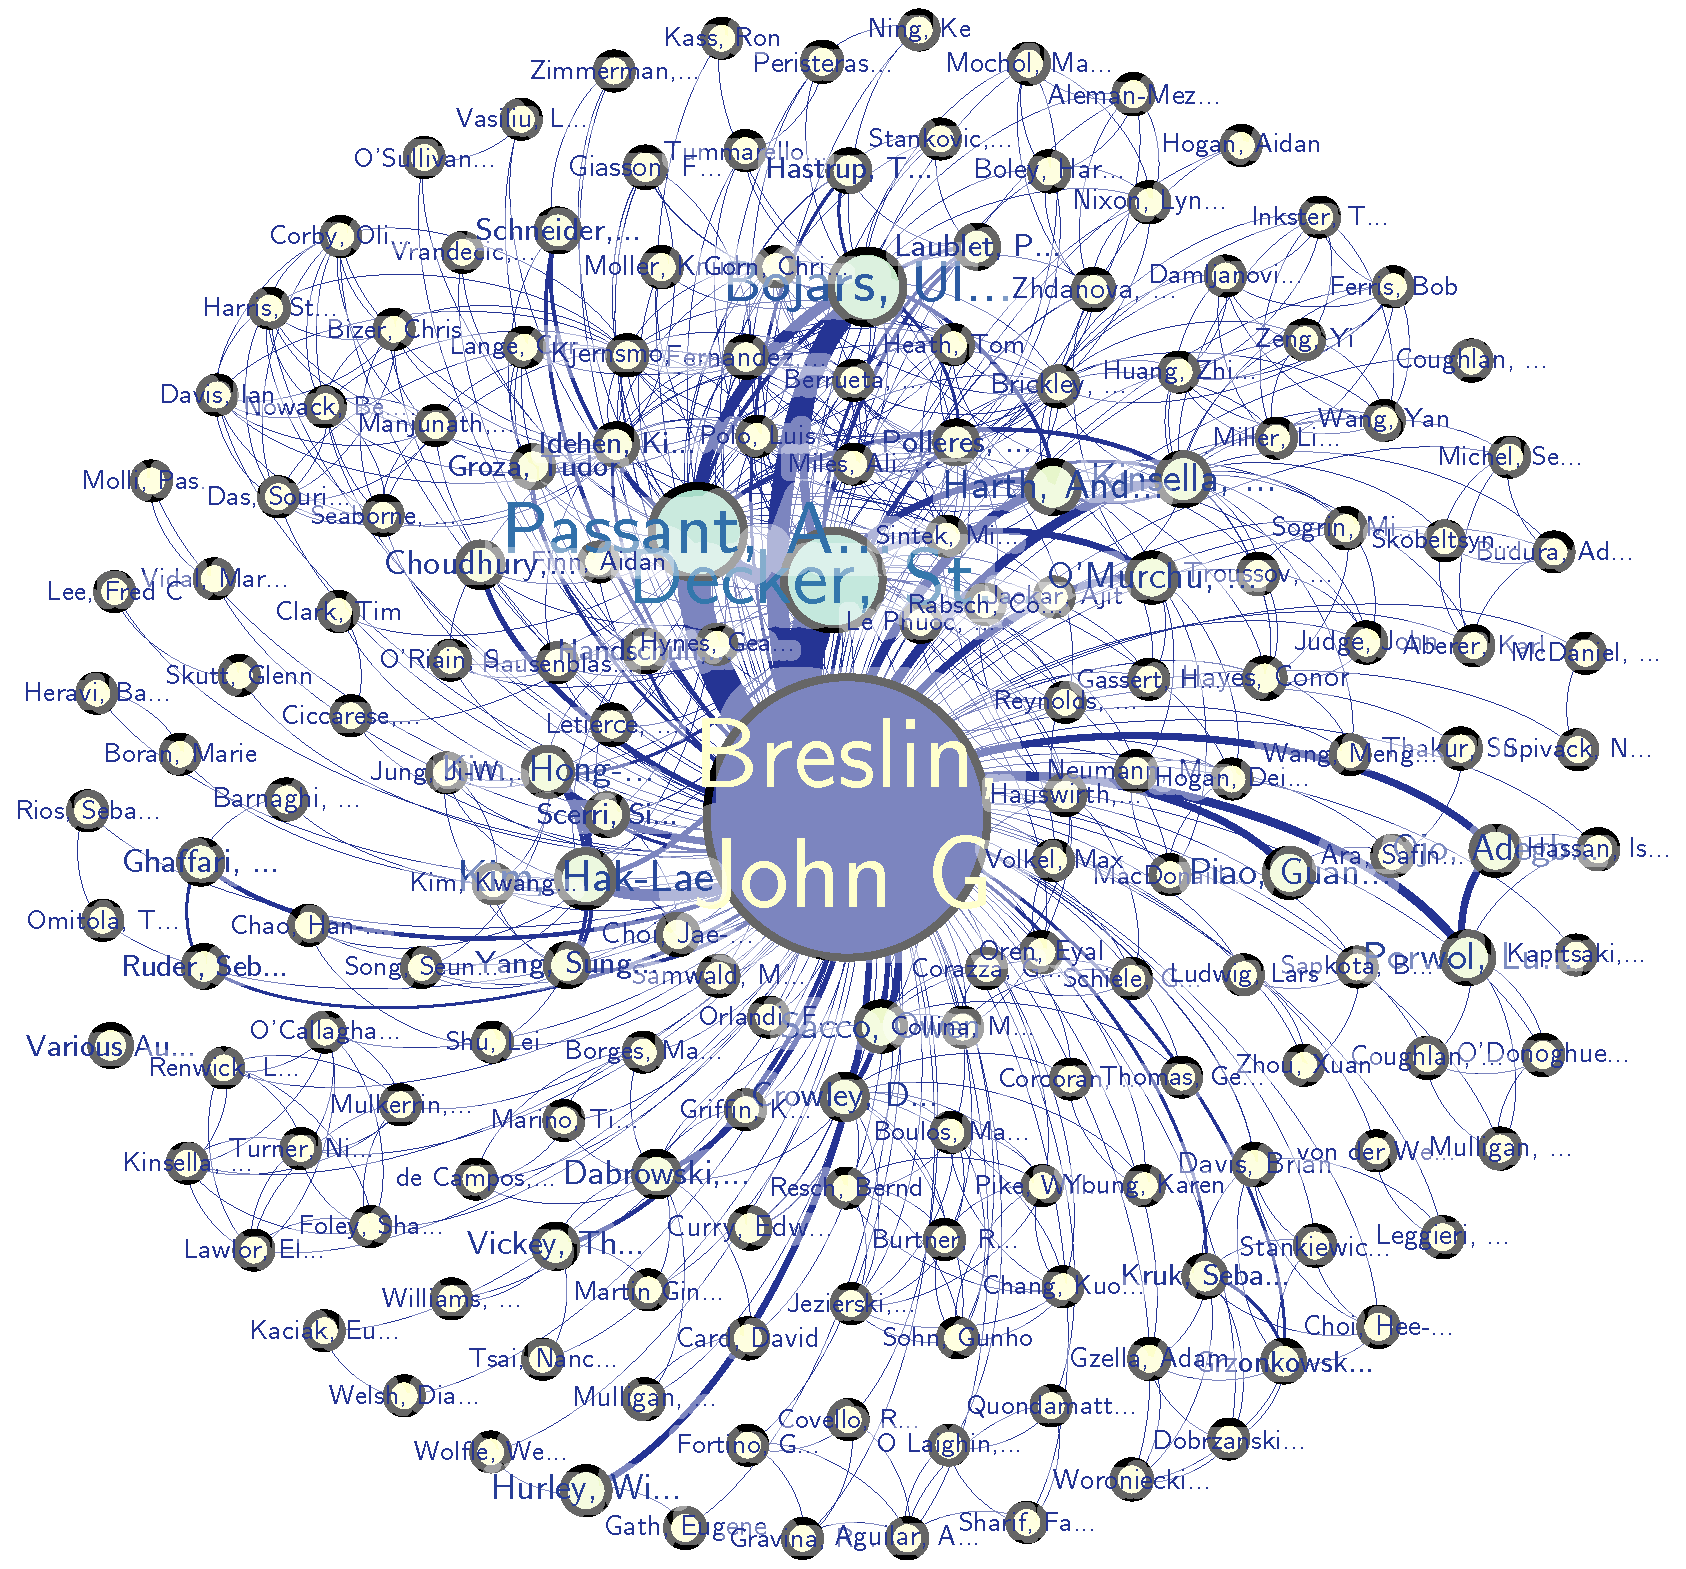
\includegraphics[width=0.48\textwidth]{figures/co-authors.pdf}
\end{center}
\caption{Co-authors}
\end{wrapfigure}

According to Google Scholar Citations, my h-index is \textbf{50} and I have over \textbf{10,000} citations. My ORCID is 0000-0001-5790-050X.

My top cited publications (with over 300 citations) are: ``Crowdsourcing, Citizen Sensing and Sensor Web Technologies for Public and Environmental Health Surveillance and Crisis Management'' (cited by 532); ``Optimizing the AC Resistance of Multilayer Transformer Windings with Arbitrary Current Waveforms'' (cited by 427); ``Towards Semantically Interlinked Online Communities'' (cited by 354); ``The Social Semantic Web'' (cited by 350); ``The Future of Social Networks on the Internet: The Need for Semantics'' (cited by 349); and ``Optimized Transformer Design: Inclusive of High Frequency Effects'' (cited by 313).

I have collaborated with about \textbf{200} other authors (see graph on right), including academic, government and industrial co-authors in organisations such as Cisco, Harvard Medical School, IBM, the US Government's Department of Health and Human Services.

My publications have been cited in patents granted to Cisco, Google, IBM, Offerpop and SAP, and patent applications by HP and Siemens, amongst others.

``Old Ireland in Colour'' co-authored with Dr Sarah-Anne Buckley is a bestselling book that brings Irish historical black and white photographs to life using a combination of artificial intelligence and human colourisation, and sold 50,000 copies in Ireland during 2020 (over \euro{}1,000,000 in sales). The sequel ``Old Ireland in Colour 2'' was also an Irish bestseller in 2021. Combined, both books have sold over 125,000 copies.

``The Social Semantic Web'' is a recommended course book in modules at Anna University Chennai, Bo\u{g}azi\c{c}i University, Institute of Technology Tallaght, National Institute of Technology Patna, Technical University of Munich, University of Bamberg, University of Vigo, Utrecht Graduate School of Humanities. It has been downloaded over 10,000 times. Two independent reviews are given below:

\medskip
\begin{quotation}``The book focuses mainly on the social Web and possibilities of its integration with the semantic Web. ... For Web developers, researchers, and graduate students, this book would be an ideal source for becoming acquainted with the evolving field of social applications on the Web. It may well fit into a seminar in information systems or related graduate study programs'' (M\'{a}ria Bielikov\'{a}, ACM Computing Reviews, September 2010)\end{quotation}

\medskip
\begin{quotation}``This book provides an easy-to-understand insight into Semantic Web and Social Web technologies and highlights research challenges when applying these technologies. ... each chapter provides a literature survey which provides an introduction state-of-the-art research from the domain. ... can be of interest for those, who consider using any of these Social Web applications in their research as well as those just want to get a solid foundation on the topic. ... IT professionals, researchers, academics and graduate students can all benefit from reading this book.'' (Frank Hopfgartner, Informer, January 2012)\end{quotation}

My Erd\H{o}s number is 4: I was a coauthor with Eugene G. Gath on DOI: 10.1109/63.838110. Eugene G. Gath was a coauthor with Thomas J. Laffey on MR1335554 (96f:11139). Thomas J. Laffey was a coauthor with LeRoy B. Beasley on MR1058113 (91f:15008). LeRoy B. Beasley was a coauthor with Paul Erd\H{o}s on MR0902513 (88j:20006).

\nocite{*}

\subsection*{Peer Reviewed Publications}

\printbibliography[type=book,title={Books},heading=bibnumbered]
\printbibliography[type=inbook,title={Book Chapters},heading=bibnumbered]
\printbibliography[type=article,title={Journal Papers},heading=bibnumbered]
\printbibliography[type=inproceedings,title={Conference and Workshop Papers},heading=bibnumbered]
\printbibliography[type=unpublished,title={Abstracts},heading=bibnumbered]

\subsection*{Non-Peer Reviewed Publications}

\printbibliography[type=report,title={Technical Reports},heading=bibnumbered]
\printbibliography[type=misc,title={Other},heading=bibnumbered]
\printbibliography[type=thesis,title={PhD Thesis},heading=bibnumbered]

%----------------------------------------------------------------------------------------

\vspace{0.2in} % Some whitespace between sections

%----------------------------------------------------------------------------------------
% EDITORSHIPS SECTION
%----------------------------------------------------------------------------------------

\section{\centerline{EDITORSHIPS}}
\sectionRule
% \vspace{15pt} % Gap between title and text
\subsection*{Journals}

\begin{itemize} \itemsep -2pt
\item E. Demidova, S. Dietze, J.G. Breslin, J. Szymanski, Special Issue on Dataset Profiling and Federated Search for Linked Data, International Journal on Semantic Web and Information Systems (IJSWIS), vol. 12, no. 3, April 2016.
\item J.G. Breslin, M. Nagarajan, Special Section on the Semantic and Social Web, Elsevier Journal of Web Semantics, vol. 18, no. 1, pp. 1-48, January 2013.
\item J.G. Breslin, D. O'Sullivan, Special Issue on Semantic Web Computing in Industry, Elsevier Computers in Industry Journal, vol. 61, no. 8, October 2010.
\end{itemize}

\subsection*{Conference and Workshop Proceedings}

\begin{itemize} \itemsep -2pt
\item M. Koubarakis, H. Alani, G. Antoniou, K. Bontcheva, J.G. Breslin, D. Collarana, E. Demidova, S. Dietze, S. Gottschalk, G. Governatori, A. Hogan, F. Lecue, E. Montiel Ponsoda, A.-C. Ngonga Ngomo, S. Pinto, M. Saleem, R. Troncy, E. Tsalapati, R. Usbeck, R. Verborgh, Joint Proceedings of the International Workshop on Artificial Intelligence for Legal Documents (AI4LEGAL 2020), the 6th Natural Language Interfaces for the Web of Data Workshop (NLIWOD 2020), the 7th International Workshop on Dataset PROFILing and Search (PROFILES 2020), the 4th Workshop on Storing, Querying and Benchmarking the Web of Data (QuWeDa 2020) and the Workshop on Semantics for Online Misinformation Detection, Monitoring, and Prediction (SEMIFORM 2020) at the 19th International Semantic Web Conference (ISWC 2020), CEUR vol. 2722, ISSN 1613-0073, November 2020. \url{http://ceur-ws.org/Vol-2722/}.
\item E. Demidova, S. Dietze, S. Gottschalk, J.G. Breslin, P. Cimiano, B. Ell, A. Lawrynowicz, L. Moss, A.-C. Ngonga Ngomo, Joint Proceedings of the 6th International Workshop on Dataset PROFIling and fEderated Search for Linked Data (PROFILES 2019) and the 1st Workshop on Semantic Explainability (SEMEX 2019) at the 18th International Semantic Web Conference (ISWC 2019), CEUR vol. 2465, ISSN 1613-0073, October 2019. \url{http://ceur-ws.org/Vol-2465/}
\item L. Koesten, E. Demidova, V. Savenkov, J.G. Breslin, O. Corcho, S. Dietze, E. Simperl, The International Workshop on Profiling and Searching Data on the Web (PROFILES and DATA:SEARCH 2018), Companion Proceedings of the 27th Web Conference 2018 (TheWebConf 2018), pp. 1479-1526, April 2018. \url{https://dl.acm.org/citation.cfm?id=3184558}
\item E. Demidova, S. Dietze, J. Szymanski, J.G. Breslin, Proceedings of the 4th International Workshop on Dataset PROFIling and fEderated Search for Linked Data (PROFILES 2017) at the 16th International Semantic Web Conference (ISWC 2017), CEUR vol. 1927, ISSN 1613-0073, September 2017. \url{http://ceur-ws.org/Vol-1927}
\item E. Demidova, S. Dietze, J. Szymanski, J.G. Breslin, Proceedings of the 3rd International Workshop on Dataset PROFIling and fEderated Search for Linked Data (PROFILES 2016) at the 13th Extended Semantic Web Conference (ESWC 2016), CEUR vol. 1597, ISSN 1613-0073, May 2016. \url{http://ceur-ws.org/Vol-1597}
% Various Authors. The Semantic Web: ESWC 2015 Satellite Events. Ed. by Fabien Gandon, Christophe Gu\'{e}eret, Serena Villata, John G Breslin, Catherine Faron-Zucker, and Antoine Zimmermann. Springer, Oct. 15, 2015. isbn: 9783319256382.
\item T. Omitola, J.G. Breslin, P. Barnaghi (eds.), Proceedings of the 6th Workshop on Semantics for Smarter Cities (S4SC 2015) at the 14th International Semantic Web Conference (ISWC 2015), CEUR vol. 1630, ISSN 1613-0073, Bethlehem, Philadelphia, USA, October 2015. \url{http://ceur-ws.org/Vol-1630}
\item E. Demidova, S. Dietze, J. Szymanski, J.G. Breslin, B. Berendt, L. Dragan, L. Hollink, M. Luczak-Roesch, Joint Proceedings of the 3rd International Workshop on Dataset PROFIling and fEderated Search for Linked Data (PROFILES 2015) and the 5th International Workshop on Using the Web in the Age of Data (USEWOD 2015) at the 12th Extended Semantic Web Conference (ESWC 2015), CEUR vol. 1362, ISSN 1613-0073, May 2015. \url{http://ceur-ws.org/Vol-1362}
\item P. De Leenheer, J.G. Breslin, H. Alani, R.R. de Querol, K.E. Kappler, Proceedings of the 1st International IFIP Working Conference on Value-Driven Social Semantics \& Collective Intelligence (VaSCo 2013) at the 5th International ACM Web Science Conference (WebSci 2013), CEUR vol. 1357, ISSN 1613-0073, May 2015. \url{http://ceur-ws.org/Vol-1357}
\item T. Omitola, J.G. Breslin, P. Barnaghi (eds.), Proceedings of the 5th Workshop on Semantics for Smarter Cities (S4SC 2014) at the 13th International Semantic Web Conference (ISWC 2014), CEUR vol. 1280, ISSN 1613-0073, Trentino, Italy, October 2014. \url{http://ceur-ws.org/Vol-1280}
\item P. Molli, J.G. Breslin, M.E. Vidal, Proceedings of the 3rd Workshop on Semantic Web Collaborative Spaces (SWCS 2014) at the 13th International Semantic Web Conference (ISWC 2014), CEUR vol. 1275, ISSN 1613-0073, Trentino, Italy, October 2014.  \url{http://ceur-ws.org/Vol-1275}
\item E. Demidova, S. Dietze, J. Szymanski, J.G. Breslin, Proceedings of the 1st International Workshop on Dataset PROFIling and fEderated Search for Linked Data (PROFILES 2014) at the 11th Extended Semantic Web Conference (ESWC 2014), CEUR vol. 1151, ISSN 1613-0073, May 2014. \url{http://ceur-ws.org/Vol-1151}
% Various Authors. Proceedings of the Sixth International Conference on Weblogs and Social Media. Ed. by John G Breslin, Nicole B Ellison, James G Shanahan, and Zeynep Tufekci. AAAI Press, June 2012. isbn: 9781577355564.
\item J.G. Breslin, U. Boj\={a}rs, A. Passant, S. Fern\'{a}ndez (eds.), Proceedings of the 4th International Workshop on Social Data on the Web (SDOW 2011) at the 10th International Semantic Web Conference (ISWC 2011), CEUR vol. 830, ISSN 1613-0073, Bonn, Germany, October 2011. \url{http://ceur-ws.org/Vol-830}
\item J.G. Breslin, U. Boj\={a}rs, A. Passant, S. Fern\'{a}ndez (eds.), Proceedings of the 3rd International Workshop on Social Data on the Web (SDOW 2010) at the 9th International Semantic Web Conference (ISWC 2010), CEUR vol. 664, ISSN 1613-0073, Washington, DC, USA, Shanghai, China, November 2010. \url{http://ceur-ws.org/Vol-664}
\item J.G. Breslin, U. Boj\={a}rs, A. Passant, S. Fern\'{a}ndez (eds.), Proceedings of the 2nd International Workshop on Social Data on the Web (SDOW 2009) at the 8th International Semantic Web Conference (ISWC 2009), CEUR vol. 520, ISSN 1613-0073, Washington, DC, USA, October 2009. \url{http://ceur-ws.org/Vol-520}
\item J.G. Breslin, U. Boj\={a}rs, A. Passant, S. Fern\'{a}ndez (eds.), Proceedings of the 1st International Workshop on Social Data on the Web (SDOW 2008) at the 7th International Semantic Web Conference (ISWC 2008), CEUR vol. 405, ISSN 1613-0073, Karlsruhe, Germany, October 2008. \url{http://ceur-ws.org/Vol-405}
\item M. Mochol, A.V. Zhdanova, L.J.B. Nixon, J.G. Breslin, A. Polleres (eds.), Proceedings of The 3rd International ExpertFinder Workshop on Personal Identification and Collaborations: Knowledge Mediation and Extraction (PICKME 2008) at the 7th International Semantic Web Conference (ISWC 2008), CEUR vol. 403, ISSN 1613-0073, Karlsruhe, Germany, October 2008. \url{http://ceur-ws.org/Vol-403}
\item A.V. Zhdanova, L.J.B. Nixon, M. Mochol, J.G. Breslin (eds.), Proceedings of The 2nd International ExpertFinder Workshop on Finding Experts on the Web with Semantics (FEWS 2007) at the 6th International Semantic Web Conference and the 2nd Asian Semantic Web Conference (ISWC 2007 + ASWC 2007), CEUR vol. 290, ISSN 1613-0073, Busan, Korea, November 2007. \url{http://ceur-ws.org/Vol-290}
\end{itemize}


%----------------------------------------------------------------------------------------

\vspace{0.2in} % Some whitespace between sections

%----------------------------------------------------------------------------------------
% FUNDING SECTION
%----------------------------------------------------------------------------------------

\section{\centerline{FUNDING}}
\sectionRule
\subsection*{Funding as Budget Holder}

\begin{longtable}{ p{2 cm} | p{2 cm} | p{2 cm} | p{2 cm} | p{7 cm} }
Period & Funding agency & \euro{} Own / University of Galway total & Role & Title of research project / programme \\
\hline
% LaTeX is generated from my Funding spreadsheet on Google Sheets
2024-2025 & TÉRI & \euro{}92,642 & FI & VistaMilk Research Ireland Centre / Taighde Éireann - Research Ireland Centre \\
2023-2026 & EC & \euro{}108,572 / \euro{}434,289 & PI & Decarbonisation and Digitalisation of Atlantic Ports (ENEPORTS) (with Umair Ul Hassan and Pau Farr\`{a}s) / Interreg Atlantic Area \\
2023-2026 & EC & \euro{}225,781 & PI & Advanced Digital Technologies for the Blue Economy (ADT4Blue) / Interreg Atlantic Area \\
2023-2023 & G\'{E}ANT & \euro{}30,000 & Co-PI & Secure Data Management for Multi-Cloud Environments (SecMC) (with Nitesh Bharot) / Innovation Programme \\
2023-2026 & EC, EI & \euro{}1,143,029 & Co-PI & Data2Sustain / European Digital Innovation Hubs \\
2022-2027 & SFI & \euro{}399,201 & Co-PI & Sustainable, Green and Energy Efficient Artificial Intelligence for Autonomous Systems (SustAIn) (with Steven Davy at TU Dublin) / Frontiers for the Future \\
2022-2025 & HEA & \euro{}861,000 & PI & MSc in AgInnovation / Springboard+ \\
2021-2022 & HEA & \euro{}220,580 & PI & MSc in AgInnovation (with Brendan Allen) / Springboard+ \\
2020-2023 & EC & \euro{}217,750 & Co-PI & OntoCommons / Horizon 2020 DT-NMBP-39-2020 \\
2020-2021 & SFI & \euro{}87,475 & Co-PI & Distributed Ledger Technology Identifying and Solving Public Service Problems Using the Blockchain (with Kosala Yapa Bandara and Subhasis Thakur) / SFI Public Service Fellowship Programme \\
2020-2021 & HEA & \euro{}263,220 & PI & MSc in AgInnovation (with Brendan Allen) / Springboard+ \\
2020-2021 & SFI & \euro{}220,000 & Co-PI & The First Digital Biomarker in Female Reproductive Health, Uncloaking Endometriosis and Filling the Diagnostic Gap (Cail\'{i}n) (with Siobh\'{a}n Kelleher) / SFI Future Innovator Prize \\
2019-2025 & SFI & \euro{}350,151 / \euro{}12,000,000 & Co-PI & Insight Centre for Data Analytics / Research Centre Phase 2 \\
2019-2023 & EC & \euro{}194,239 & PI & Smart Manufacturing Advanced Research Training (SMART 4.0) / Marie Sk\l{}odowska-Curie Action COFUND \\
2019-2022 & DBEI & \euro{}384,089 & Co-PI & Cooperative Energy Trading System (CENTS) (with Subhasis Thakur) / Disruptive Technologies Innovation Fund \\
2019-2021 & EC & \euro{}41,480 & Co-PI & Circular HRM (with Paul Flynn) / EACEA Erasmus+ Strategic Partnerships \\
2019-2020 & HEA & \euro{}245,970 & PI & MSc in AgInnovation / Springboard+ \\
2018-2024 & SFI & \euro{}377,249 & FI & VistaMilk Centre for Precision Pasture-Based Dairying / Research Centre \\
2018-2021 & EC & \euro{}219,227 & Coordinator & Startup Skills for Researchers and Innovators in Entrepreneurship Development (STARTED) / EACEA Erasmus+ Programme Knowledge Alliances \\
2018-2019 & EI & \euro{}12,430 & PI & Dynamic Cybersecurity Infrastructure Simulation (with Subhasis Thakur) / Coordinator Proposal Preparation Support \\
2018-2019 & HEA & \euro{}185,707 & Co-PI & MSc in AgInnovation (with Paul Flynn) / Springboard+ \\
2018-2019 & IERC & \euro{}45,707 & Co-PI & P2P Energy Trading Using Blockchain (EnerPort) (with Subhasis Thakur and Barry Hayes) / T2 Collaborative Research Programme (top-ranked proposal) \\
2018-2018 & SFI, IBM & \euro{}42,397 & Co-PI & Blockchain and FinTech (with Subhasis Thakur) / Targeted Project \\
2017-2023 & SFI & \euro{}1,093,767 & Co-PI & Confirm Centre for Smart Manufacturing / Research Centre \\
2017-2018 & HEA & \euro{}171,086 & PI & Postgraduate Diploma in TechInnovation / Springboard+ \\
2015-2019 & IRC, AYLIEN & \euro{}96,000 & PI & PhD on Neural Transfer Learning / Employment Based Postgraduate Programme \\
2015-2017 & IRC, AYLIEN & \euro{}48,000 & PI & MApplSc on Streaming Sentiment Analysis / Employment Based Postgraduate Programme \\
2015-2015 & EI & \euro{}15,000 & PI & Privacy Preference Framework / Commercial Case Feasibility Grant \\
2015-2015 & EI & \euro{}11,452 & PI & Digital Age Narrative Trajectories / Coordinator Proposal Preparation Support \\
2014-2019 & SFI & \euro{}785,806 / \euro{}12,450,025 & Co-PI & Insight Centre for Data Analytics / Research Centre \\
2014-2018 & SFI, SAP & \euro{}175,000 & Co-PI & PhD on Modelling in OSNs for Recommendation / Targeted Project \\
2014-2017 & EC & \euro{}30,000 / \euro{}90,000 & Co-PI & A Collaboration Ecosystem Enabling EU Creative SMEs to Exchange Multimedia Content and Create Multiplot, Interactive Apps for Children, Curated According to Reader Ability and Educational Value (Q-Tales) (with Michael Hogan and Tony Hall) / Horizon 2020 ICT-18-2014 \\
2014-2015 & EI & \euro{}12,000 & PI & Biology-Like Monitoring of Innovation Strategies / Coordinator Proposal Preparation Support \\
2014-2015 & EI & \euro{}12,920 & PI & Citizen Activism to Improve Law Enforcement and Policing by Communities / Coordinator Proposal Preparation Support \\
2014-2015 & EI & \euro{}12,000 & PI & Protecting Privacy in the Social Web / Coordinator Proposal Preparation Support \\
2014-2014 & SFI & \euro{}97,049 & PI & Social Media Repository of Ireland (with Royal Irish Academy) / Technology Innovation Development Award \\
2013-2017 & EC & \euro{}0 & Co-Proposer & KEYSTONE Semantic Keyword-Based Search on Structured Data Sources / COST Action \\
2013-2014 & SFI & \euro{}200,000 & FI & Insight Centre for Data Analytics / Research Centre \\
2013-2014 & EC & \euro{}291,925 & PI & Eurapp Study on the EU App Economy (with Gigaom Research) / Startup Europe Study \\
2013-2013 & IRC & \euro{}9,995 & PI & researchers.ie / N/A \\
2012-2012 & SFI & \euro{}23,700 & PI & AAAI ICWSM-12 Support Grant / Conferences and Workshops Programme \\
2010-2010 & SFI & \euro{}6,501 & PI & Visiting Researcher at the National Institute for Informatics in Tokyo / Short Term Travel Fellowship Grant \\
2010-2014 & IRC, ACE & \euro{}72,009 & PI & PhD on Physical Activity and Social Networks / Enterprise Partnership Scheme \\
2009-2011 & IRC & \euro{}48,006 & PI & MEngSc on Social Networks for Irish Researchers / Government of Ireland Postgraduate Scholarship \\
2008-2013 & SFI & \euro{}822,000 / \euro{}14,889,398 & Co-PI & DERI L\'{i}on II / Centre for Science, Engineering and Technology \\
2008-2009 & EI, TouristR & \euro{}197,184 & PI & TripPlanr / Innovation Partnership \\
2008-2008 & EI & \euro{}4,132 & PI & TouristR Background Research / Innovation Voucher \\
2003-2003 & NUI Galway & \euro{}6,500 & PI & Web-Based Magnetic Component Design / Millennium Fund \\
\end{longtable}

\subsection*{Other Funding}

\begin{tabular}{ p{2 cm} | p{2 cm} | p{2 cm} | p{2 cm} | p{7 cm} }
Period & Funding agency & \euro{} Total & Role & Title of research project / programme \\
\hline
% Add PorterShed a hAon
2018 & EI & \euro{}2,487,000 & Non-Profit & Galway City Innovation District: Building Two / Regional Enterprise Development Fund \\
2017 & EI & \euro{}20,000 & Non-Profit & Galway City Innovation District: Building Two / Regional Enterprise Development Fund Feasibility Grant \\
2017 & EI & \euro{}670,000 & Non-Profit & Galway City Innovation District: NDRC at PorterShed / Regional Accelerator Development Scheme \\
2015 & EI & \euro{}178,417 & Non-Profit & Galway City Innovation District: PorterShed / Community Enterprise Initiative \\
\end{tabular}

\subsection*{Funding Reviewer}

\begin{itemize} \itemsep -2pt
\item Ulysses Scheme for the Irish Research Council [2024]
\item Accelerator Jury Member (Evaluator) for the European Innovation Council (EIC)[2023]
\item Horizon 2020 Soft Landing Project for the European Commission (Monitor) [2019]
\item Research Foundation - Flanders (FWO) [2018]
\item College of Expert Reviewers for the European Science Foundation (ESF) [2017]
\item Horizon 2020 Call ICT-11-2017 for the European Commission (Evaluator) [2017]
\item French National Institute for Research in Computer Science and Control (INRIA) Project Team [2013]
\item National Fund for Scientific and Technological Development (FONDECYT) of the Chilean Government Commission for Scientific and Technological Development (CONICYT) [2012]
\item Expeditions in Computing for the US National Science Foundation (NSF) [2008]
\item Innovation Partnership Programme for Enterprise Ireland [2007]
\end{itemize}

%----------------------------------------------------------------------------------------

\vspace{0.2in} % Some whitespace between sections

%----------------------------------------------------------------------------------------
% COLLABORATIONS SECTION
%----------------------------------------------------------------------------------------

\section{\centerline{COLLABORATIONS}}
\sectionRule
\subsection*{Industry Collaborations}

\begin{figure}[b]
\begin{center}
\includegraphics[width=0.5\textwidth]{figures/Neelie.png}
\end{center}
\caption{With EC Vice President Neelie Kroes at the launch of the Eurapp Final Report}
\end{figure}

\begin{itemize} \itemsep -2pt
\item ``Eurapp'' with Gigaom Research
\begin{itemize} \itemsep -2pt
\item First EC-funded study to size the EU app economy in terms of developer / support jobs and app sales / contract work revenues
\item Study was carried out with the research arm of major online technology publisher Gigaom, and was part of the EC's Startup Europe initiative
\item Crowdsourcing was used to come up with solutions to the main bottlenecks encountered in the EU app economy
\item Final report was launched by European Commission VP Neelie Kroes in February 2014
\end{itemize}
\item ``SIOC'' with Opera, OpenLink Software, Asemantics, etc.
\begin{itemize} \itemsep -2pt
\item Social data framework is one of the most widely used Semantic Web vocabularies on the Web
\item W3C Member Submission was made in collaboration with the above companies and a collection of academic partners
\item SIOC has been deployed on over 65,000 websites with 35 million data instances, including energy.gov, london.gov.uk, www.iq.harvard.edu, software.intel.com, and others that use the Drupal 7 CMS
\item SIOC is used in more than 100 software systems including Yahoo! SearchMonkey, Boeing inSite, Vodafone ZYB, OpenLink Virtuoso and Talis Engage
\item The words `SIOC' and `semantic' occur together in over \textbf{3,060} publications
\end{itemize}
\item ``S2E'' with Cisco
\begin{itemize} \itemsep -2pt
\item Semantic mapping was created for core XMPP stanzas, physical presences (e.g. sensor devices, geolocation), social network profiles and desktop activities in RDF using existing standard vocabularies including SIOC, FOAF, SSN (and SPITFIRE), PIMO
\item Served as inspiration for the social semantic framework used in Cisco Quad, developed by Cisco R\&D in Galway
\end{itemize}
\item ``Social Semantic Spreading Activation'' with IBM
\begin{itemize} \itemsep -2pt
\item Small collaboration with IBM's LanguageWare group that led to published work in the book ``Why Context Matters''
\item Galaxy tool from IBM used spreading activation on social semantic data to cluster people and topics
\end{itemize}
\end{itemize}

\subsection*{Academic Collaborations}

\begin{itemize} \itemsep -2pt
\item ``SWAN/SIOC'' with Massachusetts General Hospital / Harvard Medical School
\begin{itemize} \itemsep -2pt
\item Project to align the SWAN (Semantic Web Applications in Neuromedicine) and SIOC (Semantically Interlinked Online Communities) ontologies
\item Aimed to provide a complete model to represent scientific discourse in online communities at different levels of granularity (discourse elements and content items)
\end{itemize}
\item ``KEYSTONE'' with Universit\'{a} degli Studi di Modena e Reggio Emilia and others
\begin{itemize} \itemsep -2pt
\item Co-authored this COST Action proposal on semantic keyword search on structured data, which grew to include 28 countries
\item Coordinated dissemination of this project's results, working with Chair Francesco Guerra and the rest of the Executive Scientific Board
\end{itemize}
\item ``Social Media Archive of Ireland'' with the Digital Repository of Ireland at the Royal Irish Academy
\begin{itemize} \itemsep -2pt
\item Project exploring the feasibility of creating an archive of social media-related activity that surrounds important national debates and events
\item Aims to facilitate the selection and preservation of social media from an Irish context, as well as looking at the legal and ethical issues surrounding this preservation
\item Should be useful to those looking at how current or historical events in a particular region are reflected in the combination of social and mainstream media
\end{itemize}
\item ``Semantic Tagging'' with Seoul National University
\begin{itemize} \itemsep -2pt
\item Created a semantic model for tag clouds and a tag sharing / exchange service based on this model
\end{itemize}
\item Various collaborators on interdisciplinary research papers, projects and proposals at NUI Galway
\begin{itemize} \itemsep -2pt
\item College of Arts, Social Sciences, \& Celtic Studies: \\ Dr Tony Hall, Dr Michael Hogan, Dr Niall \'{O} Dochartaigh, Dr Conch\'{u}r \'{O} Giollag\'{a}in, Dr Denis O'Hora, Dr Henrike Rau, Dr Kiran Sarma
\item College of Business, Public Policy, \& Law: \\ Dr Thomas Acton, Mr. Michael Campion, Dr Johanna Clancy, Dr Kieran Conboy, Dr Christine Domegan, Dr Natasha Evers, Dr Eoin Whelan
\item College of Engineering \& Informatics: \\ Dr Peter Corcoran, Dr Kathryn Cormican, Dr Edward Curry, Prof. Stefan Decker, Dr Conor Hayes, Dr Myra Lydon, Dr Adegboyega Ojo, Prof. David O'Sullivan, Prof. Dietrich Rebholz-Schuhmann, Karen Young
\item College of Medicine, Nursing, \& Health Sciences: \\ Dr Dympna Casey, Prof. Kathleen Murphy, Dr Fabio Quondamatteo
\item College of Science: \\ Prof. Afshin Samali, Prof. Charles Spillane
\end{itemize}
\end{itemize}

\subsection*{Government Collaborations}

\begin{itemize} \itemsep -2pt
\item ``HADA+PPO/PPM'' with US Government Health and Human Services
\begin{itemize} \itemsep -2pt
\item Leveraged NUI Galway's privacy preference management for linked data architectures, specifically for the area of health and hospital-related linked data
\item Deployed on a system that published Linked Government Data and required an access control framework to filter who could access specific data
\item Worked with the late George Thomas and his team in Washington DC on this project
\item This work resulted in a data.gov article\footnote{\url{http://www.data.gov/communities/node/116/blogs/20731}} and subsequent press release
\end{itemize}
\item ``researchers.ie'' with the Irish Research Council
\begin{itemize} \itemsep -2pt
\item Index of Irish-based researcher profiles, initially of students funded by IRCSET (later the Irish Research Council)
\item Demonstrated to Professor Paddy Cunningham, Ireland's Chief Scientific Adviser to the Taoiseach, and other stakeholders at the end of the project
\end{itemize}
\item ``Galway Traffic Forum'' with Galway City Council, etc.
\begin{itemize} \itemsep -2pt
\item Initiated efforts to create a social platform for this group to address transportation bottlenecks in Galway City
\item Part of the Galway Transport Forum and Better Transport for Galway Initiative
\item Worked with key stakeholders from the Galway City Council, Galway Chamber of Commerce, NUI Galway Civil Engineering, and Engineers Ireland
\end{itemize}
\end{itemize}

%----------------------------------------------------------------------------------------

\vspace{0.2in} % Some whitespace between sections

%----------------------------------------------------------------------------------------
% POSTGRADUATE/STAFF SUPERVISION SECTION
%----------------------------------------------------------------------------------------

\section{\centerline{POSTGRADUATE/STAFF SUPERVISION}}
\sectionRule
\subsection*{Current Supervisions}

\begin{itemize} \itemsep -2pt
\item Rory Ward, PhD, Data Science Institute, School of Engineering, University of Galway, 2021 -- Present. Funder: CRT-AI (Taighde \'{E}ireann - Research Ireland)
\item Hassan Khan, PhD, Data Science Institute, School of Engineering, University of Galway, 2023 -- Present. Funder: Sustain (Taighde \'{E}ireann - Research Ireland)
\end{itemize}

\subsection*{Current Co-Supervisions as Primary Supervisor}

\begin{itemize} \itemsep -2pt
\item Yasar Khan, PhD, Data Science Institute, School of Engineering, University of Galway, 2016 -- Present. Examiners: Co-Supervisor: Mathieu d'Aquin. Funder: Insight (Taighde \'{E}ireann - Research Ireland)
\end{itemize}

\subsection*{Current Co-Supervisions as Secondary Supervisor}

\begin{itemize} \itemsep -2pt
\item Rishabh Chandaliya, PhD, Data Science Institute, School of Computer Science, University of Galway, 2021 -- Present. Co-Supervisor: Martin Serrano. Funder: i3-Market (Horizon 2020)
\item Atiya Usmani, PhD, Data Science Institute, School of Computer Science, University of Galway, 2018 -- Present. Co-Supervisor: Edward Curry. Funder: Insight (Taighde \'{E}ireann - Research Ireland)
\end{itemize}

\subsection*{Previous Supervisions}

% Dates in comments are those of their vivas
\begin{itemize} \itemsep -2pt
\item Dr Sebastian Ruder, ``Neural Transfer Learning for Natural Language Processing'', PhD, Data Science Institute, College of Engineering \& Informatics, NUI Galway, 2015 -- 2019. Examiners: Ivan Titov, Paul Buitelaar. Funder: Irish Research Council and AYLIEN Ltd. % 26 February 2019
\item Dr Guangyuan Piao, ``Semantics-Aware User Modeling and Recommender Systems in Online Social Networks'', PhD, Data Science Institute, College of Engineering \& Informatics, NUI Galway, 2014 -- 2018. Examiners: Harith Alani, Dietrich Rebholz-Schuhmann. Funder: Insight (Science Foundation Ireland) and SAP % 2 July 2018
\item Marie Boran, ``Understanding Social Media Adoption in the Irish Scientific Community and its Relevance to Interpreting Altmetrics'', MApplSc, Insight Research Institute, College of Engineering \& Informatics, NUI Galway, 2012 -- 2015. Examiners: Tope Omitola, Conor Hayes. Funder: DERI/Insight (Science Foundation Ireland)
\item Julie Letierce, ``Understanding If and How the Web Improves Scientific Communication Between its Stakeholders'', MEngSc, DERI, College of Engineering \& Informatics, NUI Galway, 2009 -- 2012. Examiners: Padraig Murphy, Stefan Decker. Funder: DERI (Science Foundation Ireland)
\item Dr Smitashree Choudhury, ``A Social Context-Enabled Framework for the Semantic Enrichment and Integration of Web Videos'', PhD, DERI, College of Engineering \& Informatics, NUI Galway, 2006 -- 2011. Examiners: Lora Aroyo, Stefan Decker. Funder: DERI (Science Foundation Ireland) % 4 November 2011
\item Dr Sheila Kinsella, ``Augmenting Social Media Items with Metadata using Related Web Content'', PhD, DERI, College of Engineering \& Informatics, NUI Galway, 2006 -- 2011. Examiners: Fabien Gandon, Stefan Decker. Funder: DERI (Science Foundation Ireland) % 30 August 2011
\item Gerard Cahill, ``A Web Portal Powered by Social Network Data for Irish Researchers'', MEngSc, DERI, College of Engineering \& Informatics, NUI Galway, 2009 -- 2011. Examiners: Robin Teigland, Stefan Decker. Funder: Irish Research Council for Science, Engineering and Technology
\item Dr Uldis Bojars, ``The SIOC MEthodology for Lightweight Ontology Development'', PhD, DERI, College of Engineering \& Informatics, NUI Galway, 2004 -- 2009. Examiners: Chris Bizer, Stefan Decker. Funder: DERI (Science Foundation Ireland) % November 2009
\item Dr Hak-Lae Kim, ``Leveraging a Semantic Framework for Augmenting Social Tagging Practices in Heterogeneous Content Sharing Platforms'', PhD, DERI, College of Engineering \& Informatics, NUI Galway, 2006 -- 2009. Examiners: Tom Gruber, Philippe Laublet, Stefan Decker. Funder: DERI (Science Foundation Ireland) % September 2009
\end{itemize}

\subsection*{Previous Co-Supervisions as Primary Supervisor}

\begin{itemize} \itemsep -2pt
\item Dr Jefkine Kafunah, ``Uncertainty-Aware Fault Diagnosis for Safety-Related Industrial Systems'', PhD, Data Science Institute, School of Engineering, University of Galway, 2019 -- 2023. Examiners: Yi Wang, Edward Curry. Co-Supervisor: Ali Intizar. Funder: Confirm and Insight (Science Foundation Ireland) % 17 November 2023
\item Duc-Duy Nguyen, ``On-Demand Decentralised Internet of Things Collectability Marketplace Using Crowdsensing'', MEngSc, Data Science Institute, School of Engineering, University of Galway, 2017 -- 2022. Examiners: Damon Berry, Edward Curry. Co-Supervisors: Mathieu d'Aquin, Alessandro Adamou, Ali Intizar. Funder: Confirm (Science Foundation Ireland)
\item Dr Bharath Sudharsan, PhD, Data Science Institute, School of Engineering, NUI Galway, 2019 -- 2022. Co-Supervisor: Ali Intizar. Examiners: Thomas Runkler, Edward Curry. Funder: Confirm (Science Foundation Ireland) % 20 May 2022
\item Dr Safina Showkat Ara, ``Exploration Algorithms for Discoverable and Undiscoverable Decentralised Online Social Networks'', PhD, Data Science Institute, School of Engineering, NUI Galway, 2015 -- 2021. Co-Supervisor: Subhasis Thakur. Examiners: Antonio Moreno, Peter Corcoran. Funder: Insight (Science Foundation Ireland) % 9 December 2021
\item Dr Hoan Nguyen Mau Quoc, ``A Scalable Spatio-temporal Query Processing for Linked Sensor Data'', PhD, Data Science Institute, School of Engineering, NUI Galway, 2012 -- 2019. Examiners: Axel Polleres, Juan Miguel G\'{o}mez Berb\'{i}s, Mathieu d'Aquin. Co-Supervisor: Danh Le Phuoc. Funder: OpenIOT (FP7) % 11 December 2019
% School of Engineering, 1 September 2019
% College of Engineering \& Informatics, 31 August 2019
\item Huy Le Van, ``Near Real-Time Data Warehousing of Linked Streams'', MApplSc, Data Science Institute, College of Engineering \& Informatics, NUI Galway, 2013 -- 2018. Examiners: Antonio Jara, Mathieu d'Aquin. Co-Supervisors: Martin Serrano, Danh Le Phuoc. Funder: Fed4FIRE (FP7) and OpenIOT (FP7)
\item Dr Ted Vickey, ``Just Tweet It: The Collection, Processing, Classification and Analysis of 2 Million Fitness Tweets'', PhD, Data Science Institute, Discipline of Electrical \& Electronic Engineering, NUI Galway, 2010 -- 2018. Examiners: Alan Smeaton, Gear\'{o}id \'{O} Laighin. Co-Supervisors: Cedric Bryant, Kathleen Martin Ginis, Stephen Kinsella. Funder: Irish Research Council for Science, Engineering and Technology and American Council on Exercise % 13 June 2018
\item Dr Lukasz Porwol, ``The Duality of e-Participation - A Model and Technical Infrastructure to Study and Harness Social Media-Based Participation'', PhD, Insight Research Institute, College of Engineering \& Informatics, NUI Galway, 2010 -- 2016. Co-Supervisor: Adegboyega Ojo. Examiners: Soon Ae Chun, Murray Scott. Funder: DERI/Insight (Science Foundation Ireland) and Cloud4SOA
\item Dr Myriam Leggieri, ``Distributional Semantics for Sensors Linking and Selection'', PhD, Insight Research Institute, College of Engineering \& Informatics, NUI Galway, 2010 -- 2015. Examiners: Steffen Staab, Michael Schukat. Co-Supervisors: Brian Davis, Alexandre Passant. Funder: SPITFIRE % 24 November 2015
\item Dr Owen Sacco, ``Trust-Aware Privacy Preferences for Information Sharing on the Web of Data'', PhD, DERI, College of Engineering \& Informatics, NUI Galway, 2010 -- 2014. Examiners: Mathieu d'Aquin, Stefan Decker. Co-Supervisors: Alexandre Passant, Alessandra Mileo. Funder: Irish Research Council for Science, Engineering and Technology and Cisco Systems % 13 June 2014
\item Dr Antonio Aguilar, ``Design and Evaluation of an Automated Algorithm for Cardiac Risk Stratification'', PhD, Discipline of Electrical \& Electronic Engineering, NUI Galway, 2009 -- 2013. Examiners: Ronney Panerai, Gerard Hurley. Co-Supervisors: Gear\'{o}id \'{O} Laighin, Fabio Quondamatteo. Funder: Ambient Assisted Living Joint Programme % 7 April 2014
\item Dr Fabrizio Orlandi, ``Profiling User Interests on the Social Semantic Web'', PhD, DERI, College of Engineering \& Informatics, NUI Galway, 2010 -- 2014. Examiners: Fabien Gandon, Stefan Decker. Co-Supervisor: Alexandre Passant. Funder: Irish Research Council for Science, Engineering and Technology and Cisco Systems % 31 March 2014
\item Dr Jodi Schneider, ``Enabling Reuse of Arguments and Opinions in Open Collaboration Systems'', PhD, DERI, College of Engineering \& Informatics, NUI Galway, 2009 -- 2013. Examiners: Simon Buckingham Shum, Siegfried Handschuh. Co-Supervisors: Alexandre Passant, Stefan Decker. Funder: DERI (Science Foundation Ireland) % 1 October 2013
\item Ina O'Murchu, ``Connecting Local Community Groups Using Semantic Technologies'', MSc, DERI, College of Engineering \& Informatics, NUI Galway, 2004 -- 2006. Examiners: Sung-Kook Han, Stefan Decker. Co-Supervisor: Stefan Decker. Funder: DERI (Science Foundation Ireland)
\end{itemize}

\subsection*{Previous Co-Supervisions as Secondary Supervisor}

\begin{itemize} \itemsep -2pt
\item Dr Anupa Shyamlal de Silva, ``PCN: Next-Gen Monetary System Infrastructure'', PhD, Data Science Institute, School of Engineering, University of Galway, 2020 -- Present. Examiners: Najmul Islam, Malika Bendechache. Co-Supervisor: Subhasis Thakur. Funder: VistaMilk (Taighde \'{E}ireann - Research Ireland) % 18 October 2024
\item Dr Abdul Wahid, ``Leveraging Hybrid Deep Learning and Generative Modelling to Accurately Estimate the Remaining Useful Life of Mechanical Systems'', PhD, Data Science Institute, School of Engineering, University of Galway, 2019 -- 2024. Examiners: Hua-Liang Wei, Ihsan Ullah. Co-Supervisor: Ali Intizar. Funder: Confirm (Science Foundation Ireland) % 7 February 2024
\item Dr Jaleed Khan, ``Neurosymbolic Visual Reasoning with Scene Graph Enrichment'', PhD, Data Science Institute, School of Computer Science, University of Galway, 2019 -- 2024. Examiners: Joao Leite, Matthias Nickles. Co-Supervisor: Edward Curry. Funder: CRT-AI (Science Foundation Ireland) % 30 January 2024
\item Dr Muhammad Yahya, ``Building Semantic Models and Knowledge Graphs for Intelligent Smart Manufacturing Applications'', PhD, Data Science Institute, School of Engineering, University of Galway, 2019 -- 2023. Examiners: Dimitrios Kyritsis, John McCrae. Co-Supervisor: Ali Intizar. Funder: Confirm (Science Foundation Ireland) % 4 December 2023
\item Dr Sweta Malik, ``Peer-to-Peer Energy Trading in Microgrids: A Game-Theoretic Approach'', PhD, Data Science Institute, School of Engineering, University of Galway, 2019 -- 2023. Examiners: Zita Vale, Enda Barrett. Co-Supervisors: Subhasis Thakur, Maeve Duffy. Funder: CENTS (DTIF) and Insight (Science Foundation Ireland) % 22 November 2023
\item Chan Le Van, ``Optimisation of a Linked Stream Processing Engine'', MApplSc, Insight Research Institute, College of Engineering \& Informatics, NUI Galway, 2013 -- 2016. Examiners: Emanuele Della Valle, Michael Schukat. Co-Supervisors: Alessandra Mileo, Danh Le Phuoc, Muhammad Intizar Ali. Funder: GAMBAS (FP7)
\item Dr Shane Lowe, ``The Design, Development and Validation of a Wearable Behaviour Monitor for the Autonomous Assessment of the Functional Health of Older Adults'', PhD, Discipline of Electrical \& Electronic Engineering, NUI Galway, 2009 -- 2013. Examiners: Rose Anne Kenny, Maeve Duffy. Co-Supervisor: Gear\'{o}id \'{O} Laighin. Funder: Irish Research Council for Science, Engineering and Technology and Georgia Tech Ireland
\item Alan Dunne, ``Development of a Touchscreen System for Upper Extremity Rehabilitation of Children with Cerebral Palsy'', MEngSc, Discipline of Electrical \& Electronic Engineering, NUI Galway, 2009 -- 2011. Examiners: Eugene Coyle, Gear\'{o}id \'{O} Laighin. Co-Supervisor: Gear\'{o}id \'{O} Laighin. Funder: Irish Research Council for Science, Engineering and Technology and Georgia Tech Ireland
\end{itemize}

\subsection*{Previous Supervisions of Minor Projects}

\begin{itemize} \itemsep -2pt
\item Richard Hunt, ``Using QR Codes to Improve the Touristic Experience'', MA in Digital Media, Huston School of Film and Digital Media, NUI Galway, 2013 -- 2014
\item Mary Murphy, ``A Study of Social Inclusion and the Use of Technology in Encouraging Interaction'', MA in Digital Media, Huston School of Film and Digital Media, NUI Galway, 2010 -- 2011
\item Martin Fitzgerald, ``Creating a Community-Based IPTV Channel'', MA in Digital Media, Huston School of Film and Digital Media, NUI Galway, 2006 -- 2007
\end{itemize}

\subsection*{Current Research Fellows}

\begin{itemize} \itemsep -2pt
\item Dr Subhasis Thakur
\end{itemize}

\subsection*{Current Postdoctoral Researchers/Research Associates}

\begin{itemize} \itemsep -2pt
% \item Dr Noura Alrashidy
% \item Dr Ifeoluwapo Aribilola
\item Dr Nitesh Bharot
% \item Dr Jefkine Kafunah
\item Dr Hager Saleh
\item Mafalda Santos
\item Dr Mirco Soderi
\end{itemize}

\subsection*{Current Research Assistants}

\begin{itemize} \itemsep -2pt
\item None
\end{itemize}

\subsection*{Previous Research Fellows}

\begin{itemize} \itemsep -2pt
\item Dr Priyanka Verma
\end{itemize}

\subsection*{Previous Postdoctoral Researchers/Research Associates}

\begin{itemize} \itemsep -2pt
\item Dr Kosala Yapa Bandara
\item Dr Ronan Cummins
\item Dr Maciej Dabrowski
\item Dr Aidan Finn
\item Dr Conor Hayes
\item Dr Bahareh Heravi
\item Dr Shahid Hussain
\item Dr Jeff Morgan
\item Gabriel Mullarkey
\item Dr Alexandre Passant
\item Dr Saurabh Shukla
\item Dr Lan Yang
\end{itemize}

\subsection*{Previous Research Assistants}

\begin{itemize} \itemsep -2pt
\item Arnaud Daron
\item Vignesh Kamath
\item Kamalesh Kanakaraj
\item Ajay Nair
\item Fionnt\'{a}n O'Donnell
\end{itemize}

\subsection*{Visiting Students and Professors}

\begin{itemize} \itemsep -2pt % Ordered by last visit
\item Filippo Berto, University of Milan, Italy
\item Nakul Mehta, Dr B R Ambedkar National Institute of Technology, Jalandhar, India
\item Federica Rollo, University of Modena and Reggio Emilia, Italy
\item Julien Paganelle, L'\'{E}cole d'Ing\'{e}nieurs du Centre des \'{E}tudes Sup\'{e}rieures Industrielles de Pau, France
\item Charles-Adrien Beneteau, L'\'{E}cole d'Ing\'{e}nieurs du Centre des \'{E}tudes Sup\'{e}rieures Industrielles de Pau, France
\item Giustina Ciccariello, Roma Tre University, Italy
\item Alessia Antelmi, University of Salerno, Italy
\item Karen Young, NUI Galway, Ireland
\item Matthieu Rebouh, L'\'{E}cole d'Ing\'{e}nieurs du Centre des \'{E}tudes Sup\'{e}rieures Industrielles de Pau, France
\item Nitish Mittal, Netaji Subhas Institute of Technology, India
\item Ayushi Gupta, Indira Gandhi Delhi Technical University for Women, India
\item Vanya Sharma, Indira Gandhi Delhi Technical University for Women, India
\item Karthik Aluru, Universit\'{e} Paris-Sud XI Orsay, France
\item Roberto Covello, University of Calabria, Italy
\item Tara Donoghue, University of Limerick, Ireland
\item Sergio Fern\'{a}ndez, Fundaci\'{o}n CTIC, Spain
\item Tuukka Hastrup, University of Jyv\"{a}skyl\"{a}, Finland
\item Gandhi Hernandez, Universidad Carlos III de Madrid, Spain
\item Christian Hunsen, University of G\"{o}ttingen, Germany
\item Jung Jin-Uk, Seoul National University, Korea
\item Prof. Jason Jung, Yeugnam University, Korea
\item Tiago Marino, Universidade Federal do Rio de Janeiro, Brazil
\item Mateusz Marmo{\l}owski, Technical University of Gdansk, Poland
\item Yuki Matsuoka, National Institute of Informatics, Japan
\item Thomas Schandl, Vienna University of Economics and Business, Austria
\item Daniel Villanueva, Universidad Carlos III de Madrid, Spain
\item Sungkwon Yang, Seoul National University, Korea
\end{itemize}

\subsection*{Current TechInnovate Lecturers}

\begin{itemize} \itemsep -2pt
\item Prof. W. Bernard Carlson
\item Martina O'Grady
\end{itemize}

\subsection*{Previous TechInnovate Lecturers}

\begin{itemize} \itemsep -2pt
\item Brendan Allen
\item Dr Edelle Doherty
\item Dr Paul Flynn
\item Dr Samir Vinchurkar
\end{itemize}

\subsection*{Previous TechInnovate Fellows}

\begin{itemize} \itemsep -2pt
\item Capt. Neil Curran
\item Ronan Boyle
\item Leon Butler
\item Dr Paul Flynn
\item Niamh Lynch
\item Jane O'Connor
\item Gregory Payne
\item Kelsey Roberts
\item Ciara Shields
\end{itemize}

%----------------------------------------------------------------------------------------

\vspace{0.2in} % Some whitespace between sections

%----------------------------------------------------------------------------------------
% POSTGRADUATE COMMITTEES SECTION
%----------------------------------------------------------------------------------------

\section{\centerline{POSTGRADUATE COMMITTEES}}
\sectionRule
\subsection*{External Examiner}

\begin{itemize} \itemsep -2pt
% \item Syed Muhammad Raza Naqvi, PhD, University of Technology Tarbes Occitanie Pyr\'{e}n\'{e}es, 2025. Supervisor: Hedi Karray. Examiners: John G. Breslin.
\item Dr Rosario Davide D'Amico, ``Cognitive Digital Twins: Enabling Holistic Asset Management Through Semantic Interoperability and Human Expertise Integration'', PhD, Cranfield University, 2024. Supervisors: John Ahmet Erkoyuncu, Pavan Addepalli. Examiners: John G. Breslin, Weisi Guo. % 17 June 2024
\item Tha\'{i}s Quintas de Arcanjo, ``Sending Cryptocurrency Over Mobile Applications'', MSc, Dublin City University, 2019. Supervisor: Ray Walshe. Examiner: John G. Breslin.
\item Dr Saud Aljaloud, ``An Investigation into the Performance of Regular Expressions within the SPARQL Query Language'', PhD, University of Southampton, 2018. Supervisor: Nicholas Gibbins. Examiner: John G. Breslin. % 8 August 2018
\item Dr Zide Meng, ``Temporal and Semantic Analysis of Richly Typed Social Networks from User-Generated Content Sites on the Web'', PhD, Universit\'{e} Nice Sophia Antipolis, 2016. Supervisors: Fabien Gandon, Catherine Faron-Zucker. Examiners: John G. Breslin, Frederique Laforest, Frederic Precioso. % 7 November 2016
\item Dr Richard Hosking, ``Arguing over Copyright: An eScience Tool for Understanding and Reasoning over Copyright in Digital Scholarship'', PhD, University of Auckland, 2016. Supervisor: Mark Gahegan. Examiners: John G. Breslin, David Nichols.
\item Dr Gregoire Burel, ``Community and Thread Methods for Identifying Best Answers in Online Question Answering Communities'', PhD, Open University, 2015. Supervisor: Harith Alani. Examiners: John G. Breslin, Stefan Rueger. % 17 November 2015
\item Dr Carlos Vicient, ``Automatic, Unsupervised and Domain-Independent System for Extracting Features and Topics from Documents and Microblogs'', PhD, Universitat Rovira i Virgili, 2015. Supervisor: Antonio Moreno. Examiner: John G. Breslin.
\item Dr Nicolas Marie, ``Linked Data-Based Exploratory Search'', PhD, Universit\'{e} Nice Sophia Antipolis, 2014. Supervisors: Myriam Ribi\'{e}re, Fabien Gandon. Examiners: John G. Breslin, Harald Sack, Guy Melan\c{c}on.
\item Dr Hannes Ebner, ``Supporting Loose Forms of Collaboration: Using Linked Data to Realize an Architecture for Collective Knowledge Construction'', PhD, KTH Royal Institute of Technology, 2014. Supervisors: Marko Turpeinen and Ambj{\"o}rn Naeve. Examiners: John G. Breslin (Opponent), Teemu Leinonen, \r{A}sa Smedberg, Marcelo Milrad.
\item Andreas Textor, ``Semi-Automatic Management of Knowledge Bases Using Formal Ontologies'', MSc, Cork Institute of Technology and University of Applied Sciences in Wiesbaden, 2011. Supervisors: Jeanne Stynes, Reinhold Kr{\"o}ger. Examiner: John G. Breslin.
\end{itemize}

\subsection*{Internal Examiner}

\begin{itemize} \itemsep -2pt
\item Dr Rajdeep Sarkar, ``Exploring Structured and Unstructured Knowledge Sources for Developing Domain-Specific Chatbots'', PhD, 2023. Supervisor: John McCrae. Examiners: Ond\v{r}ej Du\v{s}ek, John G. Breslin. % 19 May 2023
\item Dr Meshari Alshammari, ``Bidirectional Inverter with Improved Light Load Efficiency for Integration in a Hybrid AC/DC Distribution System in Buildings'', PhD, 2023. Supervisor: Maeve Duffy. Examiners: Esteban Sanchis, John G. Breslin. % 3 February 2023
\item Dr Bassim Mahbooba, ``Enhancing Trust in Detecting Security Threats using Machine Learning Approaches and Its Relevance in Internet of Things Scenarios'', PhD, 2022. Supervisor: Martin Serrano. Examiners: Antonio Jara, John G. Breslin. % 21 October 2022
\item Dr Maman Ahmad Khan, ``Enhancing the Situational Awareness of the Active Distribution Network'', PhD, 2022. Supervisor: Barry Hayes. Examiners: Marco Pau, John G. Breslin. % 25 April 2022
\item Dr Tarek Zaarour, ``Adaptive Knowledge Extraction and Loose Semantic Coupling in Multimedia Publish/Subscribe Overlay Networks'', PhD, 2022. Supervisor: Edward Curry. Examiners: Boris Koldehofe, John G. Breslin. % 4 April 2022
\item Dr Asma Khatoon, ``Design and Development of Smart Contract System for Blockchain Based Applications'', PhD, 2021. Supervisor: Peter Corcoran. Examiners: Anirban Sengupta, John G. Breslin. % 26 August 2021
\item Dr Heike Vornhagen, ``Supporting Sense-Making Experiences of City Dashboards: A Design Solution'', PhD, 2021. Supervisors: Karen Young, Brian Davis, Manel Zarrouk. Examiners: Rob Brennan, John G. Breslin. % 23 August 2021
\item Dr Qaiser Mehmood, ``Efficient Path Query Approaches Over Distributed Linked Data'', PhD, 2021. Supervisor: Mathieu d'Aquin. Examiners: Pascal Molli, Thomas Riechert, John G. Breslin.
\item Felipe Arruda Pontes, ``Energy- and Speed-Aware Self-Adaptive Scheduler for Deep Learning Models for Multimedia Event Processing on the Cloud-Edge'', MApplSc, 2021. Supervisor: Edward Curry. Examiners: Mar\'{i}a P\'{e}rez-Hern\'{a}ndez, John G. Breslin.
\item Dr Mohan Timilsina, ``Graph-Based Diffusion Methods for Node Classification and Link Prediction'', PhD, 2020. Supervisor: Mathieu d'Aquin. Examiners: Nicola Perra, John G. Breslin.
\item Dr Lan Yang, ``Ontology Learning for Systems Engineering Body of Knowledge'', PhD, 2020. Supervisor: Kathryn Cormican. Examiners: Cecilia Haskins, John G. Breslin.
\item Dr Danielly Ferriera Oliveira DePaula, ``Design Thinking Capability Model: A Management Framework to Support Design Thinking Implementation'', PhD, 2019. Supervisor: Kathryn Cormican. Examiners: Juliana Hsuan, John G. Breslin.
\item Durre Zehra, ``Linked Open Data for Cancer Genomics'', MSc, 2019. Supervisors: Ratnesh Sahay, Mathieu d'Aquin. Examiners: Paris Vogazianos, John G. Breslin.
\item Dr Hugo Hromic, ``Detecting, Defining and Interpreting Communities in Fast Moving Social Media Platforms'', PhD, 2019. Supervisor: Conor Hayes. Examiners: Miriam Fernandez, John G. Breslin.
\item Dr Zia Ush Shamszaman, ``Enabling Smart Societies Using Social Internet of Things'', PhD, 2019. Supervisor: Ali Intizar. Examiners: Giancarlo Fortino, John G. Breslin.
\item Dr Shane Tuohy, ``Hybrid Simulation of Ethernet Based Intra-Vehicle Networks'', PhD, 2017. Supervisors: Liam Kilmartin, Edward Jones, Martin Glavin. Examiners: Nicolas Navet, John G. Breslin.
\item Dr Nur Rakhmawati, ``Evaluating and Benchmarking the Performance of Federated SPARQL Endpoints and Their Partitioning using Selected Metrics'', PhD, 2016. Supervisors: Stefan Decker, Dietrich Rebholz-Schuhmann. Examiners: S\"{o}ren Auer, John G. Breslin.
\item Dr Darren Craven, ``Low Power Strategies for Signal Compression in Ambulatory Healthcare'', PhD, 2016. Supervisors: Edward Jones, Martin Glavin, Liam Kilmartin. Examiners: Jonathon Chambers, John G. Breslin.
\item Dr Umair Ul Hassan, ``Adaptive Task Assignment in Spatial Crowdsourcing'', PhD, 2016. Supervisor: Edward Curry. Examiners: Seng Loke, John G. Breslin.
\item Dr Shejin Thavalengal, ``Contributions to Practical Iris Biometrics on Smartphones'', PhD, 2016. Supervisor: Peter Corcoran. Examiners: Kevin Bowyer, John G. Breslin.
\item Dr Souleiman Hasan, ``Loose Coupling in Heterogeneous Event-Based Systems via Approximate Semantic Matching and Dynamic Enrichment'', PhD, 2015. Supervisor: Edward Curry. Examiners: Gordon Blair, John G. Breslin.
\item Dr Muhammad Qureshi, ``Application and Analysis of Structured Data to Problems in Information Retrieval'', PhD, 2015. Supervisor: Colm O'Riordan. Examiners: Joemon Jose, John G. Breslin.
\item Dr Jun Zhang, ``High Frequency Resonant Converter with Planar Magnetics'', PhD, 2015. Supervisors: Gerard Hurley, Maeve Duffy. Examiners: Jesus Acero, John G. Breslin.
\item Dr Sabrina Kirrane, ``Linked Data with Access Control'', PhD, 2014. Supervisors: Alessandra Mileo, Stefan Decker. Examiners: Tim Finin, John G. Breslin.
\item Dr Muhammad Aftab Iqbal, ``Large Scale Data Integration of OSS Repositories for Automated Soft and Technical Factors Assessment'', PhD, 2014. Supervisors: Michael Hausenblas, Stefan Decker. Examiners: Jeff Pan, Asunci\'{o}n G\'{o}mez P\'{e}rez, John G. Breslin.
\item Dr Benjamin Heitmann, ``An Open Framework for Multi-Source, Cross-Domain Personalisation with Semantic Interest Graphs'', PhD, 2014. Supervisor: Conor Hayes. Examiners: Tommaso Dinoia, John G. Breslin.
\item Sonya Abbas, ``Reference Architecture and Implementation of a Linked Geospatial Data Infrastructure'', MSc, 2014. Supervisor: Adegboyega Ojo. Examiners: Matteo Palmonari, John G. Breslin.
\item Divanshu Gupta, ``Scalable Facet Synthesis for Relational Faceted Navigation System'', MSc, 2013. Supervisors: Stefan Decker, Giovanni Tummarello, Renaud Delbru. Examiners: Fabrizio Silvestri, John G. Breslin.
\item Sajin Kumar, ``A Framework to Publish Tweets in Linked Data Web'', MSc, 2013. Supervisors: Stefan Decker, Adegboyega Ojo. Examiners: Marijn Janssen, John G. Breslin.
\item Mengjiao Wang, ``Information Fusion Methods for the Automatic Creation of User Lists in Microblogs'', MSc, 2013. Supervisor: Conor Hayes. Examiners: Matthew Rowe, John G. Breslin.
\item Dr Lei Shu, 2010, ``Streaming Data Gathering in Wireless Multimedia Sensor Networks'', PhD, 2010. Supervisor: Manfred Hauswirth. Examiners: Takahiro Hara, John G. Breslin.
\item Dr Andreas Harth, ``Exploring Linked Data on Web Scale'', PhD, 2010. Supervisor: Stefan Decker. Examiners: Karl Aberer, John G. Breslin.
\item Stephane Corlosquet, ``Bootstrapping the Web of Data with Drupal'', MSc, 2009. Supervisor: Axel Polleres. Examiners: Tim Clark, John G. Breslin.
\end{itemize}

\subsection*{Viva Chair}

\begin{itemize} \itemsep -2pt
\item Dr Mostafa Rezaeimozafar, ``Optimal Design and Scheduling for Behind-the-Meter PV Battery Energy Storage Systems'', PhD, 2024. Supervisors: Maeve Duffy, Rory Monaghan, Enda Barrett. Examiners: Georges Kariniotakis, Michael Schukat. % 12 June 2024
\item Dr Adrian \'{O} Dubhghaill, ``Natural Language Processing for Old Irish: Assessment and Development of Fundamental NLP Tasks and Techniques for Old Irish, and an Application
for the Detection of Authors in the W\"{u}rzburg Glosses'', PhD, 2024. Supervisors: John McCrae, Clodagh Downey. Examiners: Elisa Roma, Paul Buitelaar. % 10 June 2024
\item Dr Rishabh Jain, ``Child Speech Understanding and Generation via Neural ASR and TTS Models'', PhD, 2024. Supervisor: Peter Corcoran. Examiners: Mikko Kurimo, Horia Cucu, Michael Schukat. % 15 May 2024
\item Dr Shardul Suryawanshi, ``Unimodal, Multimodal and Transformational Approaches for Offensive Meme Classification: Challenges, Datasets and Models'', PhD, 2024. Supervisors: Paul Buitelaar, Mihael Arcan, Suzanne Little. Examiners: Paolo Rosso, John McCrae. % 25 March 2024
\item Dr Faisal Khan, ``Contributions to Neural Network Models and Training Datasets for Facial Depth Estimation from a Single Image'', PhD, 2023. Supervisor: Peter Corcoran. Examiners: Anil Kokaram, Michael Schukat. % 12 January 2023
\item Dr Muhammad Ali Farooq, ``Evaluations of Thermal Imaging Technology for Automotive Use Cases'', PhD, 2022. Supervisor: Peter Corcoran. Examiners: Saraju Mohanty, Martin O'Halloran. % 3 May 2022
\item Dr Mona Isazad Mashinchi, ``Dashboards for Supporting Cancer Care in Value-Based Healthcare Context: Information Needs, Design Principles and Acceptance'', PhD, 2021. Supervisors: Karen Young, Adegboyega Ojo, Frank Sullivan. Examiners: Elsa Estevez, Murray Scott.
\item Dr Alokkumar Jha, ``Semantic Knowledge Graphs to Understand Tumor Evolution and Predict Disease Survival in Cancer'', PhD, 2019. Supervisors: Mathieu d'Aquin, Ratnesh Sahay. Examiners: Maria Esther Vidal, John Newell.
\item Dr Laleh Kazemzadeh, ``Identification of Regional Interaction Patterns in Regulatory Networks'', PhD, 2017. Supervisor: Frank Barry. Examiners: Michael Schr\"{o}der, Mary Murphy.
\item Dr Mihael Arcan, ``Multilingual Enhancement of Domain-Specific Knowledge'', PhD, 2016. Supervisor: Paul Buitelaar. Examiners: Josef van Genabith, Dietrich Rebholz-Schuhmann.
\item Dr Andre Freitas, ``Schema-Agnostic Queries for Large-Schema Databases: A Distributional Semantics Approach'', PhD, 2014. Supervisor: Edward Curry. Examiners: Christopher Brewster, Paul Buitelaar.
\item Dr Sanaullah Nazir, ``Data Availability Analysis in P2P Networks'', PhD, 2012. Supervisor: Manfred Hauswirth. Examiners: Anwitaman Datta, Siegfried Handschuh.
\item Dr Ratnesh Nandan Sahay, ``An Ontological Framework for Interoperability of Health Level Seven (HL7) Applications: The PPEPR Methodology and System'', PhD, 2012. Supervisors: Axel Polleres, Ronan Fox, Manfred Hauswirth. Examiners: Jeff Pan, Alberto Fern\'{a}ndez Gil, Stefan Decker.
\item Dr Peyman Nasirifard, ``Advances in Understanding, Mining and Using People Tags'', PhD, 2012. Supervisor: Conor Hayes. Examiners: Robert Engels, Stefan Decker.
\item Dr Vinh Tuan Thai, ``Visual Exploration of Text Collections'', PhD, 2012. Supervisor: Siegfried Handschuh. Examiners: Enrico Motta, Stefan Decker.
\end{itemize}

\subsection*{Confirmation Examination Committees}

\begin{itemize} \itemsep -2pt
\item Paul Stacey, ``Interoperable Knowledge Engineering Techniques for Ultra-Constrained Heterogeneous Geo-Observational Sensor Systems'', Dublin Institute of Technology. Supervisor: Damon Berry. Examiners: John G. Breslin.
\end{itemize}

\subsection*{Graduate Research Committees}

\begin{itemize} \itemsep -2pt
\item College of Arts, Social Sciences, \& Celtic Studies
\begin{itemize}
\item School of Education: Annette Cosgrove
\item School of Political Science \& Sociology: Mike Hynes
\end{itemize}
\item College of Business, Public Policy, \& Law
\begin{itemize}
\item Discipline of Business Information Systems, School of Business \& Economics: Colin Callinan
\end{itemize}
\item College of Science \& Engineering:
\begin{itemize}
\item Discipline of Electrical \& Electronic Engineering: Andrei Barcovschi, Ethan Delaney, Sean Dooney, Kevin Farrell, Seyedroohollah Hosseini, Jaroslaw Jakubowicz, Asma Khatoon, Paul Kielty, Fearghal Kineavy, Tudor Nedelcu, David Newell, Mostafa Rezaeimozafar, Shejin Thavalengal, Tirui Wu, Jun Zhang, Wei Zhao
\item Discipline of Information Technology: Stephen Bradshaw
\item Discipline of Mechanical Engineering (Industrial Engineering): Fabiola Cortes Chavez, Neda Makrooni, Sagar Shinde
\item Data Science Institute: Salma Abdulaziz, Alex Acquier, Erik Aumayr, Andrea Barraza, Milena Caires, Sarah Carter, Lin Clark, Stephane Corlosquet, Tobias Daudert, Feng Gao, Benjamin Heitmann, Aidan Hogan, Maciej Janowski, Yasar Khan, Waqas Khawaja, Sabrina Kirrane, Julie Letierce, Bassim Mahbooba, Mona Mashinchi, Qaiser Mehmood, Nakul Mehta, Duc-Duy Nguyen, Bianca Pereira, Thu-Le Pham, Felipe Arruda Pontes, Narumol Prangnawarat, Nur Aini Rakhmawati, Hazem Safwat, Zia Ush Shamszaman, Annanda Sousa, Atiya Usmani, Piyush Yadav, Tarek Zaarour, Omnia Zayed, Durre Zehra
\item Plant \& AgriBiosciences Research Centre, School of Natural Sciences: Zewdy Gebremedhin
\end{itemize}
\end{itemize}

%----------------------------------------------------------------------------------------

\vspace{0.2in} % Some whitespace between sections

%----------------------------------------------------------------------------------------
% INVITED TALKS SECTION
%----------------------------------------------------------------------------------------

\section{\centerline{INVITED TALKS, TUTORIALS AND PANELS}}
\sectionRule
\vspace{15pt}

\begin{figure}[htbp]
\begin{center}
\includegraphics[width=0.5\textwidth]{figures/Stanford.jpg}
\end{center}
\caption{Invited talk at Stanford University in 2013}
\end{figure}

\subsection*{Invited Talks}

I have given invited talks on my research, teaching and community activities at various prestigious locations including Stanford University, University of Chile, US Library of Congress, University of Maryland Baltimore County, Applied Physics Laboratory at Johns Hopkins University, New York Times, Tsinghua University, and Open University.\\

\begin{enumerate} \itemsep -2pt
\item ``Cognitive Digital Twins for Industry 4.0/5.0'', Keynote Talk at the 14th International Workshop of Advanced Manufacturing and Automation (IWAMA 2024), Kuming, China [Online], 11th October 2024.
\item ``Entrepreneurship and the Blue Economy'', Talk at the ADT4Blue Blue Economy Challenges in Ireland Workshop [Online], 22nd June 2024.
\item ``Five Years Using GenAI to Bring Ireland's History to Life in Colour'', Talk at the SPECTRA GenAI Hackathon, PorterShed, Galway, 22nd June 2024.
\item ``Entrepreneurship Development for Industry'', Invited Talk at the Innovation and Entrepreneurship as a Concept Webinar [Online], Construct Innovate and Engineers Ireland West Region, 26th March 2024.
\item ``Disruptive Technologies: Collaborations Between the Insight Centre, Third-Level Education and Industry in Ireland'', Invited Talk at the Thematic Workshop on Disruptive Technologies to the Service of Regional Innovation Ecosystems, CODIL Interreg Europe, \'{U}dar\'{a}s na Gaeltachta, Na Forbacha, 19th March 2024.
\item ``Cognitive Digital Twins for Industry 4.0'', Keynote Talk at the Huawei Global Software Technology Summit, Dublin, 2nd June 2023.
\item ``Behind Old Ireland in Colour'', Invited Talk for the Public Record Office of Northern Ireland [Online], 31st March 2023.
\item ``Behind Old Ireland in Colour'', Invited Talk at the University College Cork Computer Science Seminar Series [Online], 10th February 2023.
\item ``Bringing the Past Back to Life: The Science and Engineering Behind Old Ireland in Colour'', Invited Talk to Engineers Ireland Thomond Region [Online], 19th January 2023. \url{https://www.youtube.com/watch?v=ZBN3vq55nHc}
\item ``Behind Old Ireland in Colour'', Invited Talk to the CollabArchive Project, Public Record Office of Northern Ireland [Online], 16th November 2022.
\item ``The OntoCommons Ecosystem (OCES) and Ontology Communities'', Keynote Talk to the OntoCommons Demo and Use Case Workshop, Stuttgart, Germany [Hybrid], 8th November 2022.
\item ``Old Ireland in Colour'' (with Sarah-Anne Buckley), Invited Talk to Glen Eira Libraries, Melbourne, Australia [Online], 26th May 2022.
\item ``Teaching Researchers and Innovators How to Create Startups'', Invited Talk to the Trinity College Dublin (TCD) Postgraduate Certificate in Innovation and Entrepreneurship [Online], 12th May 2022.
\item ``Teaching Researchers and Innovators How to Create Startups'', Keynote Talk at the South East Technological University (SETU) Research Postgraduate Conference 2022 [Online], 6th May 2022.
\item ``Old Ireland in Colour 2'' (with Sarah-Anne Buckley), Manchester and Lancashire Family History Society [Online], 2nd December 2021.
\item ``Old Ireland in Colour 2'' (with Sarah-Anne Buckley), Irish American Heritage Museum [Online], 24th November 2021. \url{https://www.youtube.com/watch?v=AOsvI4BTGNQ}
\item ``Old Ireland in Colour 2'' (with Sarah-Anne Buckley), Museum of Childhood Ireland [Online], 27th October 2021.
\item ``Old Ireland in Colour 2'' (with Sarah-Anne Buckley), Kildare Readers Festival [Online], 16th October 2021.
\item ``Artificial Intelligence for Image/Video Colourisation and Enhancement'', NUI Galway KPMG Summer School [Online], 14th June 2021.
\item ``Book Talk: Old Ireland in Colour'' (with Sarah-Anne Buckley), Maine Irish Heritage Center [Online], 6th June 2021.
\item ``Let's C in JCT: Our History in Colour'', Junior Cycle for Teachers (JCT) Support Service [Online], 28th May 2021.
\item ``Old Ireland in Colour'', Trasna na T\'{i}re [Online], 7th December 2020. \url{https://www.trasnanatire.ie/?wix-vod-video-id=i7M8YMCUFUw&wix-vod-comp-id=comp-kb431v45}
\item ``The PorterShed Story'', Ascent: The Rise of Galway City's Innovation District, Meyrick Hotel, Galway, 16th May 2019.
\item ``Smartups'', Invited Talk to \'{U}dar\'{a}s na Gaeltachta and Junior Achievement Ireland's Company Programme National Finalists, \'{A}r\'{a}s na Gaeilge, NUI Galway, 2nd April 2019.
\item ``Creativity, Innovation and Entrepreneurship in Higher Education'', Invited Talk at CELT, NUI Galway, 30th January 2019.
\item ``Who Is Your Customer?'', Invited Talk to Irish SAP.iO Accelerate Participants, PorterShed, Galway, 23rd November 2018.
\item ``Building the Galway Startup Ecosystem'', Invited Talk to the SAP.iO Venture Partners Team, Potsdam, Germany, 24th October 2018.
\item ``Go to Market and COCA'', Invited Talk to SAP.iO Accelerate Teams, Potsdam, Germany, 24th October 2018.
\item ``Technology Innovation'', Invited Talks to the Enterprise Ireland High Potential Start-Up Team, Mervue, Galway and East Point, Dublin, 12th June 2018 and 18th September 2018.
\item ``Accelerating Regional Entrepreneurship'', Invited Talk to the Enterprise Subgroup of the Atlantic Economic Corridor Taskforce, Mayo County Council, Claremorris, 30th May 2018.
\item ``TRICS: Teaching Researchers and Innovators How to Create Startups'', Keynote Talk at the 14th Annual Conference of the International Society for Design and Development in Education (ISDDE 2018), Galway, 29th May 2018. \url{https://www.slideshare.net/Cloud/trics-teaching-researchers-and-innovators-how-to-create-startups-99513726}
\item ``Collaborative Leadership to Increase the Northern \& Western Region's Innovation and Entrepreneurship Capacity'', Northern \& Western Region Masterclass in Collaborative Leadership, The Glasshouse Hotel, Sligo, 25th May 2018. \url{https://www.slideshare.net/Cloud/collaborative-leadership-to-increase-the-northern-western-regions-innovation-and-entrepreneurship-capacity-99513736}
\item ``Innovation Districts and Innovation Hubs'', Wexford Town Innovation District, The Gallery at Green Acres, Wexford, 3rd May 2018.
\item ``Disciplined Entrepreneurship'', Course on Applying Innovation, University of Minho, Portugal, 23rd March 2018.
\item ``Imeachta\'{i} Nu\'{a}la\'{i}ochta agus Fiontra\'{i}ochta san Ollscoil agus san Iarthar'', Roinn Fiontra\'{i}ochta agus Fosta\'{i}ochta, \'{U}dar\'{a}s na Gaeltachta, Na Forbacha, 14\'{u} M\'{i} na Nollag 2017.
\item ``Entrepreneurship is in Our DNA'', NWRA/WDC One Region One Vision Annual Conference 2017, 28th October 2017. \url{https://www.slideshare.net/Cloud/entrepreneurship-is-in-our-dna}
\item ``What Can You Do for Your Customer?'', Invited Talk to the BonBillo Social Impact Incubator, Impact Hub, Boston, 14th October 2017.
\item ``Innovation Ecosystems'', Invited Talk to the College of Medicine, Nursing \& Health Sciences, NUI Galway, 26th September 2017.
\item ``Disciplined mHealth Entrepreneurship, Invited Talk at the mHealth Conference 2017, NUI Galway, 15th June 2017. \url{http://www.slideshare.net/Cloud/disciplined-mhealth-entrepreneurship}
\item ``Innovation Districts and Innovation Hubs'', Innovation Hubs Briefing to TDs and Senators, Leinster House, Dublin, 1st February 2017. \url{https://www.slideshare.net/Cloud/innovation-districts-and-innovation-hubs}
\item ``Innovation and Entrepreneurship: Tips and Tricks'', Invited Talk to IRUPA / Connacht Rugby Players, PorterShed, Galway, 2nd November 2016. \url{https://www.slideshare.net/Cloud/innovation-and-entrepreneurship-tips-tools-and-tricks}
\item ``Growing Galway's Startup Community'', Invited Talk to the Social Sciences Research Centre Conference 2016, ILAS, NUI Galway, 20th October 2016. \url{https://www.slideshare.net/Cloud/growing-galways-startup-community}
\item ``Startup Community: What Galway Can Do Next'', Bank of Ireland Workbench Launch, Bank of Ireland, Mainguard Street, Galway, 12th August 2015. \url{https://www.slideshare.net/Cloud/startup-community-what-galway-can-do-next}
\item ``Searching for Startups'', Keynote Talk at the 5th KEYSTONE MC Meeting and Winter WG Meeting, Aix-Marseille Universit\'{e}, Marseille, France, 23rd February 2016. \url{https://www.slideshare.net/Cloud/searching-for-startups}
\item ``Adding More Semantics to the Social Web'', Invited Talk to the Semantic Web and Ontology Special Interest Group, National Institute of Informatics, Tokyo, Japan, 10th July 2015. \url{https://www.slideshare.net/Cloud/adding-more-semantics-to-the-social-web}
\item ``Communities and Tech: Build Which and What Will Come?'', Invited Talk at Techgate, Junior Chamber International Galway, Galway, Ireland, 3rd December 2014. \url{https://www.slideshare.net/Cloud/communities-and-tech-build-which-and-what-will-come}
\item ``Data Analytics and Industry-Academic Partnerships: An Irish Perspective'', Keynote Talk at the Business Intelligence Workshop (BIWO 2014), Santiago, Chile, 14th August 2014. \url{https://www.slideshare.net/Cloud/data-analytics-and-industryacademic-partnerships-an-irish-perspective-37987502}
\item ``Eurapp'', Invited Talk at Workshop on Tech Entrepreneurs: The Path to Success, Digital Agenda Assembly 2013, NDRC, Dublin, Ireland, 20 June 2013.
\item ``Innovation Caf\'{e} Talk'', Invited Talk at the TCD-UCD-QUB Joint Graduate Certificate Lunchtime Speaker Series, The Innovation Academy, Dublin, Ireland, 17th April 2013. \url{https://www.slideshare.net/Cloud/john-breslin-at-the-innovation-academy}
\item ``Engaging Citizens in Research and Innovation: Opportunities and Challenges Afforded by Social Media'', Invited Talk at the European Intersectoral Summit on Research and Innovation, Trinity College Dublin, Ireland, 26th February 2013. \url{https://www.slideshare.net/Cloud/engaging-citizens-in-research-and-innovation-opportunities-and-challenges-afforded-by-social-media}
\item ``dW/dI: How a Small Country Like Ireland Can Make a Big Difference to the World (and a Bit About a `Professor Entrepreneur')'', Invited Talk at the European Entrepreneurship and Innovation Thought Leaders Seminar Series, Stanford University, USA, January 2013. \url{https://www.slideshare.net/Cloud/europreneurs}
\begin{itemize} \itemsep -2pt
\item Slides from this talk have been viewed over 8,000 times, and also generated significant interest on social media
\end{itemize}
\item ``Social Semantic Web'', Invited Talk at Innovation at the Verge: Computational Models of Physical / Virtual Space Interaction, Lorentz Center, Leiden, The Netherlands, 18th December 2012. \url{https://www.slideshare.net/Cloud/the-social-semantic-web-15712355}
\item ``Social Media for Charities'', Invited Talk at Fundraising Ireland, Galway, Ireland, September 2012. \url{https://www.slideshare.net/Cloud/social-media-for-charities-14332460}
\item ``Breaking Down Walls in Enterprise with Social Semantics'', Keynote Talk at the International Workshop on New Trends in Service Oriented Architecture for massive Knowledge processing in Modern Enterprise (SOA-KME 2012) at CISIS 2012, Palermo, Italy, July 2012. \url{https://www.slideshare.net/Cloud/breaking-down-walls-in-enterprise-with-social-semantics}
\item ``Lots of SIOC Data: Now What?'', Invited Talk at the IFIP Working Group 12.7 on Social Networking Semantics and Collective Intelligence, VU University, Amsterdam, 26th April 2012. \url{https://www.slideshare.net/Cloud/20110426a-amsterdam-ifipsnsci}
\item ``Social Media: Making It Work for You'', Invited Talk at the Irish Times Innovation Roadshow, Galway, 29th November 2011. \url{https://www.slideshare.net/Cloud/social-media-making-it-work-for-you-10381200}
\item ``Dealing with Information Overload'', Invited Talk at Mayo 2040, Castlebar, Ireland, November 2011. \url{https://www.slideshare.net/Cloud/dealing-with-information-overload-10202433}
\item ``SIOC Tactics'', Invited Talk at the Web Science Summer School, Galway, Ireland, July 2011. \url{https://www.slideshare.net/Cloud/sioc-tactics-gaining-acceptance-for-a-semantic-web-vocabulary-on-the-social-web}
\item ``Social Media: Making It Work for You'', Invited Talk at the HPSU Skillnet Turning Online Networking into Real Business Symposium, Galway, 11th November 2010. \url{https://www.slideshare.net/Cloud/social-media-making-it-work-for-you-5740048}
\item ``The SIOC Project'', Invited Talk at the Federated Social Web Summit, Portland, Oregon, July 2010. \url{https://www.slideshare.net/Cloud/sioc}
\item ``The Social Semantic Web'', Invited Talk at New York Times R\&D, June 2010. \url{https://www.slideshare.net/Cloud/the-social-semantic-web-new-york-times-edition-4650198}
\item ``The Social Semantic Web'', Invited Talk at University of Maryland Baltimore County, Maryland, USA, June 2010. % Not online
\item ``The Social Semantic Web'', Invited Talk at the New York Semantic Web Meetup, May 2010. \url{https://www.slideshare.net/Cloud/another-social-semantic-web}
\item ``The Social Semantic Web'', Invited Talk at the Washington Semantic Web Meetup, Library of Congress, Washington DC, USA, May 2010. \url{https://www.slideshare.net/Cloud/a-social-semantic-web}
\item ``Social Media and the Semantic Web'', Invited Talk to Business School Students, DCU, Dublin, Ireland, 19th February 2010. \url{https://www.slideshare.net/Cloud/social-media-and-the-semantic-web}
\item ``The Social Semantic Web'', Invited Talk at Survival, Evolution or Extinction? Shaping Our Futures, British Librarians Group (BBSLG), Dublin, Ireland, July 2009. \url{https://www.slideshare.net/BLAlib/shaping-our-futures-the-social-semantic-web}
\item ``The Social Semantic Web'', Invited Talk at the ERCIM Workshop, Dublin, Ireland, June 2009. % Not online
\item ``Enhancing the Web Experience: DERI, Social Semantic Web and SIOC'', Invited Talk at the Engineers Ireland Annual Conference, Tullamore, 24th April 2009. \url{https://www.slideshare.net/Cloud/enhancing-the-web-experience}
\item ``The Social Semantic Web'', Invited Talk during Library Ireland Week, University of Limerick, March 2009, and Invited Talk at IUISC, Galway, 5th March 2009. \url{https://www.slideshare.net/Cloud/the-social-semantic-web-1328494}
\item ``Web 2.0'', Invited Talk to Engineers Ireland Thomond Region, Limerick Institute of Technology, 2nd February 2009. % Not online
\item ``The Social Semantic Web'', Invited Talk to the IET Ireland Network and NUI Galway CompSoc, DERI, NUI Galway, 27th November 2008. \url{https://www.slideshare.net/Cloud/the-social-semantic-web-presentation}
\item ``Alumni Social Networks'', Invited Talk to the NUI Galway Alumni Board, Hodson Bay Hotel, 7th November 2008.
\item ``Learning via the Social Web'', Invited Talks at the CELT Seminar Series, NUI Galway, 27th February and 30th April 2008. \url{https://www.slideshare.net/Cloud/learning-and-the-social-web-379318}
\item ``Enabling Networked Knowledge'', Invited Talk at the Digital Government / Web and Software Research Centre, Tsinghua University, Beijing, China, April 2008. % Not online
\item ``Emerging Social Networking Technologies and Possible Implications for Libraries'', Invited Talk at the LIR HEAnet Annual Seminar, Dublin, April 2008. \url{http://lirgroup.heanet.ie/sites/default/files/Seminars/2008/JohnBreslin.ppt}
\item ``The Social Semantic Web'', Invited Talk at the Irish Web Technologies Conference (IWTC 2008), Dublin, March 2008. % Not online
\item ``Social Networking and Collaboration Tools for Enterprise 2.0'', Invited Talk at the Fidelity Investments, TerraNua and ITAG Conference on Enriching the Internet Experience, Galway, October 2007. \url{https://www.slideshare.net/Cloud/social-networking-and-collaboration-tools-for-enterprise-20}
\item ``Finding Experts Using Internet-Based Discussions in Online Communities and Associated Social Networks'', Invited Talk at the ExpertFinder Workshop, Knowledge Web Assembly, Berlin, Germany, January 2007. \url{https://www.slideshare.net/Cloud/finding-experts-using-internetbased-discussions-in-online-communities-and-associated-social-networks}
\item ``Semantic Web 2.0: Creating Social Semantic Information Spaces'', Invited Talk to the Technology Transfer Initiative (TTI) and ITAG, 30th November 2006. \url{https://www.slideshare.net/Cloud/semantic-web-20-creating-social-semantic-information-spaces}
\item ``Wiki Ireland'', Invited Talk to the Galway Heritage Forum, Galway, 12th July 2006. \url{https://www.slideshare.net/Cloud/20060712a}
\item ``Blogs and Podcasting'', Invited Talk to Masters in E-Marketing Students, DCU, Dublin, Ireland, 13th March 2006. \url{https://www.slideshare.net/Cloud/blogs-and-podcasting-378607}
\item ``Syndication and RSS'', Invited Talk at the Blogging for Business Event, IT@Cork, June 2005. \url{https://www.slideshare.net/Cloud/syndication-and-rss}
\item ``Site Interoperability Projects'', Invited Talk at the Workshop on Semantic Interoperability, Knowledge Media Institute, Open University, February 2005. \url{https://www.slideshare.net/Cloud/site-interoperability-projects-at-deri-galways-sw-cluster}
\item ``Transformer Design'', Invited Talk at Wroclaw University of Technology, Poland, 2001. % Not online
\end{enumerate}

\subsection*{Tutorials}

\begin{enumerate} \itemsep -2pt
\item John G. Breslin, ``Teaching Researchers and Innovators How to Create Startups'', ImplantSens MSCA European Training Network [Online], 18th and 19th January 2022.
\item John G. Breslin, ``From Entrepreneurship to Startups'', Technical Assistance Mission, National Erasmus+ Office, Jordan [Online], 5th and 6th October 2021. % Put online
\item John G. Breslin, ``What Can You Do for Your Customer?'', Tutorial for the BonBillo Social Impact Incubator, Online, 5th November 2018. % Not online
\item John G. Breslin, ``Disciplined Entrepreneurship'', Tutorial at Blackstone LaunchPad, NUI Galway, 6th March 2018. % Not online
\item John G. Breslin, ``Disciplined Entrepreneurship'', Tutorials at PorterShed, Galway, 27th and 28th July 2017. % Not online
\item John G. Breslin, ``Disciplined Entrepreneurship'', Tutorials at Blackstone LaunchPad, NUI Galway, 15th and 22nd March 2017. % Not online
\item John G. Breslin, Paul Flynn, ``Disciplined Entrepreneurship for AgTech Startups'', Tutorial to Plant \& AgriBiosciences Research Centre, NUI Galway, 23 November 2016. % Not online
\item John G. Breslin, Alexandre Passant, ``The Social Semantic Web'', Tutorial at the Universitat Rovira i Virgili Artificial Intelligence Seminar Series, Tarragona, Spain, April 2011. % Not online
\item John G. Breslin, Alexandre Passant, ``The Social Semantic Web'', Tutorial at the 4th International AAAI Conference on Weblogs and Social Media (ICWSM-10), Washington DC, USA, May 2010. \url{https://www.slideshare.net/Cloud/the-social-semantic-web}
\item John G. Breslin, Alexandre Passant, ``The Social Semantic Web: An Introduction'', Tutorial at DERI, NUI Galway, 2nd April 2009. \url{https://www.slideshare.net/Cloud/the-social-semantic-web-an-introduction}
\item John G. Breslin, Stefan Decker, Uldis Boj\={a}rs, ``The Future of Social Networks: The Need for Semantics'', Tutorial at the Semantic Technologies Conference, San Jose, USA, May 2008. \url{https://www.slideshare.net/Cloud/the-future-of-social-networks-on-the-internet-the-need-for-semantics}
\item Uldis Boj\={a}rs, John G. Breslin, Alexandre Passant, ``Interlinking Online Communities and Enriching Social Software with the Semantic Web'', Tutorial at the 17th International World Wide Web Conference (WWW 2008), Beijing, China, 21st April 2008. \url{https://www.slideshare.net/Cloud/interlinking-online-communities-and-enriching-social-software-with-the-semantic-web}
\item John G. Breslin, ``Semantic Web 2.0'', Tutorial for Wireless Skillnet, Dublin, Ireland, May 2007. % Not online
\item John G. Breslin, Stefan Decker, ``Semantic Web 2.0: Creating Social Semantic Information Spaces'', Tutorial at the 15th International World Wide Web Conference (WWW 2006), Edinburgh, Scotland, May 2006. \url{https://www.slideshare.net/Cloud/semantic-web-20-creating-social-semantic-information-spaces-378981}
\item John G. Breslin, Maeve Duffy, W. Gerard Hurley, ``High-Frequency Effects in Transformers and CAD Design'', Tutorials in Magnetics Design run by PEI Technologies, 1996, 2000 and 2001. % Not online
\end{enumerate}

\subsection*{Panels}

\begin{enumerate} \itemsep -2pt
% Expand out initials to names
% Add in Startup Galway fireside chats
\item John G. Breslin, Paul Cheek (MIT), ``Fundraising Strategies from Ideation to Scale'', Innovative City Workshop, PorterShed, 15th October 2024.
\item John G. Breslin, Arik Elberse (Ancient Oak Ventures), Gear\'{o}id Hynes (CitySwift), Rachel Kavanagh (Siren), Carmel McGroarty-Mitchell (Chair, Insight), Emma Meehan (Precision Sports Technology), ``The Entrepreneurial Quest'', Insight Data Connections: Seizing the Data Opportunity through Collaboration, PorterShed, 23rd August 2023.
\item John G. Breslin (Chair), Orla Flynn (Atlantic Technological University), Helen McBreen (Atlantic Bridge Ventures), Elizabeth McGloughlin (Tympany Medical), Ciar\'{a}n \'{O} h\'{O}gartaigh (University of Galway), Siobhan Roche (Science Foundation Ireland), ``Supporting Student Entrepreneurship at Third Level'', Scale Ireland Regional Startup Summit, Galmont Hotel, Galway, 25th February 2023. \url{https://www.youtube.com/watch?v=j63jZnR133Y}
\item John G. Breslin (Chair), Olivia Forde (Zap Consulting), Carmel Granahan (Unify Success), Gareth McKee (Bam Boom Cloud), Magaly Murray (Gran Grans Foods), John O'Shanahan (LeanBPI), Brian Warde (Google), ``Growing Your Business in the Digital Age'', Genesys, Galway, 26th January 2023.
\item Xabier Sarasola Aramendia (Elhuyar Foundation), Loubna Bouarfa (OKRA.ai), John G. Breslin, S\'{e}amus McAteer (Chair, AI Fund), ``Using AI to Benefit Humanity'', MIT Technology Review's Innovators Under 35 Europe, Gaoth Dobhair, County Donegal, 20th May 2022. % Add to Sesame with grants Insight
\item John G. Breslin, Isam Faik (Western University), Samuel Fosso Wamba (Toulouse Business School), John Keogh (Chair, Shantalla Inc.), Louise Manning (Royal Agricultural University), Javad Nasiry (McGill University), Diana Sabrain (OneAgrix), ``Digitalizing Food Supply Systems for Business and Global Benefits'', Convergent Innovation Webinar Series, 23rd February 2022. \url{https://www.youtube.com/watch?v=z_MjBvXAsQc} % Add to Sesame with grants Insight, Confirm and VistaMilk
\item John G. Breslin (Chair), Maggie Cusack (Munster Technological University), Simon Harris (Minister for Further and Higher Education, Research, Innovation and Science), Conor Lyden (Trustap), Kevin Marshall (Microsoft Ireland), Helen McBreen (Atlantic Bridge), John O'Halloran (University College Cork), Siobhan Roche (Science Foundation Ireland), Peter Smyth (Tyndall National Institute), ``Supporting Student Entrepreneurs and Startups at Third Level'', Scale Ireland Regional Startup Summit, 28th January 2022.
\item John G. Breslin (Chair), Gianmaria Bullegas (Perpetual Labs), Clement Jonquet (LIRMM), Martin Hepp (Bundeswehr University Munich), ``Ontology Adoption'', Ontology Commons: Addressing Challenges of the Industry 5.0 Transition, 3rd November 2021.
\item John G. Breslin, Colin Keogh (Rapid Foundation), Ciara O'Brien (Chair, Irish Times), Aoife Prendergast (Analog Devices), ``Careers in Engineering'', Irish Times Higher Options 2021, 13th October 2021.
\item John G. Breslin, Damion Dooley (Simon Fraser University), John Keogh (Chair, Shantalla Inc.), Branimir Raki\'{c} (OriginTrail), ``From Web 2 Data Silos to the Semantic Web 3'', 10th September 2021. \url{https://www.youtube.com/watch?v=dEvN3Gh_Sbk}
\item June Bolneo (Grow Remote), John G. Breslin, Justin Casimir (RISE), Bryonny Goodwin-Hawkins (NICRE), Sara Lerota (Chair, Ministry of Programming), Tasos Vasileiadis (IED), ``Innovation in Rural Areas: An Exception or a Must?'', Startup OL\'{E}, 7th September 2021.
\item June Bolneo (Grow Remote), John G. Breslin, Sara Lerota (Chair, Ministry of Programming), ``Training for Rural Communities to Develop Local Innovation Capacity'', Rural European Innovation Area Launch Event, 6th April 2021.
\item John G. Breslin, Nata Duvvury, Adrienne Gorman, John McHale, Niall Madden, Grace McCormack, ``Academic Promotions Advisory Session'', University Women's Network, NUI Galway, 21st January 2020.
\item John G. Breslin, Ken Bruton (CIT), Bill O'Leary (Chair, Confirm SFI Research Centre), Andrew Parnell (Maynooth University), Roger Richardson (Corlina), ``Digital Solutions in Manufacturing: Innovations and Value from Industry and Research Perspectives'', Industrial Internet Consortium Smart Manufacturing Forum, CIT, 23rd May 2019.
\item Paul Bohan (Schneider Electric), John G. Breslin, David Cunningham (Galway City Innovation District), Derarca Dennis (Chair, EY), Brian O'Callaghan (Alere), ``Does the Future of Finance Mean New Technology or New People?'', EY Future of Finance, Meyrick Hotel, Galway, 27th March 2019.
\item Alejtin Berisha (Universum College, Kosovo), John G. Breslin, Emilio Corchado (Startup Ol\'{e} Accelerator), Agnieszka Pugacewicz (University of Warsaw, Poland), ``Transforming Universities into Entrepreneurship Engines'', Workshop at the Startup Europe Summit, Sofia, Bulgaria, 15th November 2018.
\item John G. Breslin (Chair), David Cunningham (Priviti), Carmel McGroarty-Mitchell (C\'{U}RAM Centre for Research in Medical Devices), Jan Rutherford (University of Colorado Denver), ``Leading by Innovating'', InterTradeIreland All-Island Innovation Programme, PorterShed, Galway, 28th May 2018.
\item John G. Breslin, Siobh\'{a}n Bradley (Chair, IPA), Gerard Brady (Ibec), Brendan McCormack (President, IT Sligo), ``Accelerating Growth'', Northern \& Western Region Masterclass in Collaborative Leadership, The Glasshouse Hotel, Sligo, 25th May 2018.
\item John G. Breslin (Chair), Barry O'Sullivan (CEO, Altocloud), Joe Smyth (VP, Genesys), ``Building an AI Company from Scratch - The Altocloud Story'', Atlantec Conference '18, NUI Galway, Ireland, 24th May 2018.
\item John G. Breslin, D. Carey (Chair, Moore Institute, NUI Galway), H. Felzmann (Philosophy, NUI Galway), K. Lillington (Irish Times), N. Tosh (Philosophy, NUI Galway), ``Data Protection: Where Do We Stand?'', Moore Institute, NUI Galway, 9th April 2018.
\item John G. Breslin (Chair), P. Flynn (TechInnovate/AgInnovate), M. Mellotte (Insight), N. Walsh (Blackstone LaunchPad), ``From Idea/Invention/Innovation to Customer'', Startup Europe Comes to Universities (SEC2U), Institute for Lifecourse \& Society, NUI Galway, 24th October 2017.
\item John G. Breslin, P. Anglim (BioInnovate Ireland), E. Browne (Free Feet Medical), D. Clarke (Hatchery of Ideas), A. Rialp (Chair, Autonomous University of Barcelona), B. Woods (OCREX), ``Commercialisation of Innovation for Internationalisation: Product Before Market?'', Industry Forum at the 21st McGill International Entrepreneurship Conference, PorterShed, Galway, 30th August 2017.
\item John G. Breslin (Chair), Samantha Barry (CNN), Montaser Marai (Al Jazeera), Anne-Marie Tomchak (Mashable), ``Mobile Journalism in a Post-Truth World'', Mojocon Fringe Event, NUI Galway, 4th May 2017.
\item John G. Breslin, L. Bowen (Entrepreneurs Academy), G. Canty (Fuzion Communications), G. Duffy (Chair, Gavin Duffy \& Associates), S. Martin (MamaBud), P. O'Connell (Paddy O's Cereals), M. O'Dwyer (SwiftComply), ``Looking Forward: SMEs, Startups and Entrepreneurship'', AHECS Labour Market Task Group, National College of Ireland, 27th April 2017.
\item John G. Breslin, Maurice O'Gorman (Galway Chamber), Frank O'Keeffe (EY), Jamie Williams (Chair, EY), ``Is the Future of Finance New Technology or New People?'', EY Preparing for the Future Finance Function, Meyrick Hotel, Galway, 5th April 2017.
\item John G. Breslin, J. O'Dea (Crospon), P. O'Doherty (CEO, Electric Ireland), S. Ryan (Chair, Irish Independent), S. Roarty (N17 Brewery), ``Innovation in Practice'', IBEC Innovation Imperative, Galway, 26th May 2016.
\item John G. Breslin, P. Formica (Innovation Value Institute, NUI Maynooth), A. Jazairy (World Intellectual Property Organization), J. Roos (Future Ideas), B. Samelin (Chair, European Commission), D. van Welsum (The Conference Board), ``Innovation and Entrepreneurship'', Open Innovation 2.0 Conference, Dublin Convention Centre, Dublin, 12th June 2014.
\item John G. Breslin, A. Gerber (innocomm), M. Hynes (Chair, European Science Foundation), M. Marchiori (REIsearch), D. Piechocki (Orange Labs), ``Digital and Social Media: New Ways of Engaging Citizens in Research and Innovation'', European Intersectoral Summit on Research and Innovation, Trinity College Dublin, Ireland, 26th February 2013.
\item John G. Breslin, C. Coughlan (HP), J. Ryan (Great Place to Work Ireland), M. Sugrue (Kinesense), ``Where Are the Growth Opportunities for Ireland?'', Irish Executives Summit, Radisson SAS, Galway, 27th September 2012.
\item John G. Breslin, N. Devitt (Tweak Your Biz), F. Hannigan (Pathfinder Partners International), Z. Sheerin (Mint Digital), J. Twohig (Ahain Group), ``Social Media Panel'', Irish Executives Summit, Radisson SAS, Galway, 15th September 2011.
\item John G. Breslin, D. Collins (Jolt Online Gaming), K. Majerus (Cisco), D. McLoughlin (Chair, UCD), D. Mulley (Mulley Communications), ``Digitising Your Business Model and Exploiting New Technologies'', Digital Landscapes, University College Dublin, 3rd March 2010.
\item John G. Breslin, N. Infield (British Library), I. Manzie (Thomson Reuters), D. Meehan (Chair, Dublin City University), ``Survival, Evolution or Extinction: Shaping Our Futures'', British Business Schools Librarians Group, Dublin, 2nd July 2009.
\item John G. Breslin, E. Carey (Chair, Random Thoughts Media), C. Dillon (Microsoft), W. Luenenbuerger-Reidenbach (Edelman), B. O'Connor (PricewaterhouseCoopers), ``What is Social Media'', Futureproof Conference, Dublin, 18th June 2009.
\item John G. Breslin, J. Browne (Chair, NUI Galway), O. Daniels (Nortel), A. Devitt (Forf\'{a}s), B. O'Leary (IDA), F. \'{O} M\'{o}r\'{a}in (Enterprise Ireland), ``Research and Development: Building the Knowledge Economy'', Engineers Ireland Annual Conference, Tullamore, 23rd April 2009.
\item John G. Breslin, J. Collison (Auctomatic, now Stripe), A. Finn (Chair, DERI), N. Larkin (Relevant M), A. McDermott (LogOn.ie), T. Raftery (Tom Raftery IT), ``Send Lawyers, Guns and Money, Dad: Issues Faced by Irish Technology Startups'', BarCamp Galway, DERI, NUI Galway, 22nd September 2007.
\item John G. Breslin, B. Brown (Moli), J. Collins (Chair, Irish Times), J. Drumgoole (PutPlace), P. Lynch (Eirplay Games), J. McCormick (Xbox Live Gaming Centre), M. Taylor (eircom), ``Social Networking in Games'', GAME :ON Cyber Games Festival, Digital Hub, Dublin, 10th September 2007.
\item John G. Breslin, J. Cunningham (Chair, NUI Galway), R. Fox (DERI), M. Leyden (DERI), B. McDaniel (DERI), B. Smith (DERI), ``Founders Forum'', DERI Entrepreneurial Forum, NUI Galway, 22nd June 2007.
\item John G. Breslin, S. Decker (DERI), M. Grandinetti (Chair, MIT Sloan School of Management), A. Teodorescu (IBM Venture Capital Group), D. Wyatt (McAfee SiteAdvisor), ``Information Technology Panel'', The 7th Annual MIT Technology and Entrepreneurship Forum, MIT, Cambridge, USA, 2nd March 2007.
\end{enumerate}

\subsection*{Conference Talks}

\begin{enumerate} \itemsep -2pt
% Can I just re-reference papers from the publications.bib file instead? And add link to the presentation? See if there's a full re-cite option using the paper IDs below
% bloc2019
\item ``A Balanced Routing Algorithm for Blockchain Offline Channels using Flocking'', The 1st International Congress on Blockchain and Applications (BLOCKCHAIN '19), Avila, Spain, June 2019.
% marb2019
\item ``Collusion Attack from Hubs in the Blockchain Offline Channel Network'', The 1st International Conference on Mathematical Research for Blockchain Economy (MARBLE 2019), Fira, Santorini, Greece, 9th May 2019. \url{https://www.slideshare.net/Cloud/collusion-attack-from-hubs-in-the-blockchain-offline-channel-network}
% soci2013
\item ````I Like'' - Analysing Interactions within Social Networks to Assert the Trustworthiness of Users, Sources and Content'', The 5th IEEE International Conference on Social Computing (SocialCom 2013), Washington, DC, USA, September 2013.
\end{enumerate}
 
%----------------------------------------------------------------------------------------

\vspace{0.2in} % Some whitespace between sections

%----------------------------------------------------------------------------------------
% MEDIA COVERAGE
%----------------------------------------------------------------------------------------

\section{\centerline{MEDIA COVERAGE}}
\sectionRule
\vspace{15pt} % Gap between title and text

{\footnotesize % Start footnotesize

\begin{itemize} \itemsep -2pt
\renewcommand\labelitemi{$\circ$}
\item ``Irish brown soda bread usurps the baguette amid Ireland Week festivities in France'', Patricia Killeen, Irish Central, 7th March 2024. \url{https://www.irishcentral.com/opinion/others/ireland-week-france-2024}
\item ``New Cathaoirleach has been appointed by Gaillimh le Gaeilge'', Galway Advertiser, 22nd February 2024. \url{https://www.advertiser.ie/galway/article/140033/new-cathaoirleach-has-been-appointed-by-gaillimh-le-gaeilge}
\item ``Gradam 2024 open for nominations'', Ado Lyons, This is Galway, 14th February 2024. \url{https://thisisgalway.ie/gradam-2024-open-for-nominations/}
\item ``Old Ireland as you've never seen it before'', Irish Mail on Sunday, 17th December 2023.
\item ``In living colour'', Janine Kennedy, Irish Farmers Journal, 9th December 2023. \url{https://www3.farmersjournal.ie/entertainment/books/images-from-a-bygone-era-old-ireland-in-colour-795113}
\item ``Picture this'', Linda Maher, Irish Daily Mail, 1st December 2023.
\item ``Stunning photographs of Derry, Strabane and Donegal appear in glorious Old Ireland in Colour 3'', Kevin Mullan, Derry Journal, 29th November 2023. \url{https://www.derryjournal.com/heritage-and-retro/heritage/stunning-photographs-of-derry-strabane-and-donegal-appear-in-glorious-old-ireland-in-colour-3-4427610}
\item ``Old Ireland in Colour 3'', Around the North West with John Breslin, Highland Radio, 24th November 2023.
\item ``Roscommon images feature in Old Ireland in Colour'', Christina McHugh, Roscommon Herald, 23rd November 2023. \url{https://roscommonherald.ie/news/roscommon-images-feature-in-old-ireland-in-colour_arid-3815.html}
\item ``Amazing 1926 Ardara photo features in new Old Ireland in Colour 3 book'', Michael McHugh, Donegal Post, 20th November 2023. \url{https://www.donegallive.ie/news/local-news/1353078/amazing-1926-ardara-photo-features-in-new-old-ireland-in-colour-book-3.html}
\item ``Athlone streetscape a century ago colourised in new book'', Deirdre Verney, Westmeath Independent, 15th November 2023. \url{https://www.westmeathindependent.ie/2023/11/15/athlone-streetscape-a-century-ago-colourised-in-new-book/}
\item ``New stories, old Ireland, ancient tales'', Stephen Glennon, Tuam Herald, 8th November 2023.
\item ``Days Gonne by...'', Larissa Nolan, Irish Daily Mirror, 3rd November 2023.
\item ``Old snaps hue and improved'', Larissa Nolan, Irish Daily Star, 3rd November 2023.
\item ``In pictures: the restored images bringing long-ago Ireland to life'', Larissa Nolan, Irish Star, 3rd November 2023. \url{https://www.irishstar.com/culture/nostalgia/gallery/pictures-restored-images-bringing-long-31349018}
\item ``Stunning images capture Ireland's history in new book'', Fiona Audley, Irish Post, 27th October 2023. \url{https://www.irishpost.com/entertainment/stunning-images-capture-irelands-history-in-new-book-262674}
\item ``Record breaking book back for a stunning third edition'', Declan Varley, Galway Advertiser, 19th October 2023. \url{https://www.advertiser.ie/galway/article/138251/recordbreaking-book-back-for-a-stunning-third-edition}
\item ``Old Ireland in Colour 3: latest book breathes new life into incredible old images'', Marjorie Brennan, Irish Examiner, 17th October 2023.
\item ``Rare photos of Ulster life in early 1900s published in latest book series'', Amy Cochrane, Belfast Telegraph, 16th October 2023. \url{https://www.belfasttelegraph.co.uk/life/books/rare-photos-of-ulster-life-in-early-1900s-published-in-latest-book-series/a1460621294.html}
\item ``Postcards from the past: Old Ireland in Colour'', Life Magazine, Sunday Independent, 15th October 2023. \url{https://www.independent.ie/entertainment/books-arts/book-news/postcards-from-the-past-old-ireland-in-colour/a1322823237.html}
\item ``Book cover sparks happy memories for Cork man featured as child in old picture'', Des O'Driscoll, Irish Examiner, 13th October 2023. \url{https://www.irishexaminer.com/lifestyle/artsandculture/arid-41247334.html}
\item ``New light shed on photograph taken of Offaly woman 160 years ago'', Justin Kelly, Offaly Express, 26th September 2023. \url{https://www.offalyexpress.ie/news/local-news/1307119/new-light-shed-on-photograph-taken-of-offaly-woman-160-years-ago.html}
\item ``La gale­rie du Faou\"{e}dic connec­t\'{e}e \'{a} l'Irlande [The Faou\"{e}dic gallery connected to Ireland]'', Ouest France, 4th August 2023.
\item ``Full event programme for Culture Night 2022 in Galway city'', Michael Malone, Galway Daily, 22nd September 2022. \url{https://www.galwaydaily.com/arts-entertainment/full-event-programme-for-culture-night-2022-in-galway-city/}
\item ``Past and present come alive at \'{A}ras Eanna'', Galway City Tribune, 22nd July 2022. \url{https://connachttribune.ie/past-and-present-come-alive-at-aras-eanna/}
\item ``Two stunning exhibitions open on Inis O\'{i}rr this weekend'', Ciar\'{a}n Tierney, Galway Daily, 7th July 2022. \url{https://www.galwaydaily.com/news/two-stunning-exhibitions-open-on-inis-oirr-this-weekend/}
\item ``Blockchain agus bitcoin'', Fionnuala U\'{i} Neachtain, Iris Aniar, RT\'{E} Raidi\'{o} na Gaeltachta, 24\'{u} Bealtaine 2022.
\item ``Old Cork in Colour exhibition at Spike Island gives an illuminating look at the county's heritage'', Bill Browne, The Corkman, 15th April 2022. \url{https://www.independent.ie/regionals/cork/news/old-cork-in-colour-exhibition-at-spike-island-gives-an-illuminating-look-at-the-countys-heritage/41556728.html}
\item ``There's so much to see in this amazing photo of Cork's Coal Quay in 1900'', Yay Cork, 19th December 2021. \url{https://www.yaycork.ie/theres-so-much-to-see-in-this-amazing-photo-of-corks-coal-quay-in-1900/}
\item ``Presents that really are picture perfect'', Irish Daily Mail, 17th December 2021.
\item ``Colourising photographs: far from a black and white issue'', Pavel Barter, Sunday Times, 12th December 2021. \url{https://www.thetimes.co.uk/article/colourising-photographs-far-from-a-black-and-white-issue-nct9v85jf}
\item ``NUIG lecturers' amazing book exploring the past through AI-colourised photographs becomes Irish bestseller'', Erika Sassone, Galway Beo, 1st December 2021. \url{https://www.galwaybeo.ie/culture/nuig-lecturers-amazing-book-exploring-6288150}
\item ``Old Ireland in Colour 2'', Tom Hurley, The Avondhu, 29th November 2021.
\item ``Watch: Incredible remastered footage of Michael Collins in color'', Irish Central, 24th October 2021. \url{https://www.irishcentral.com/roots/history/rare-footage-michael-collins-color}
\item ``1920s Ireland in Colour'', Tom\'{a}s O Mainn\'{i}n, RT\'{E} Six One News and Nine O'Clock News, 24th October 2021.
\item ``Picture this'', Maeve Quigley, Irish Daily Mail, 22nd October 2021.
\item ``Old Ireland goes back for more'', Nick Mulcahy, Business Plus, 20th October 2021.
\item ``Fascinating book brings old Dublin to life with newly colourised pictures'', Brian Dillon, Dublin Live, 18th October 2021. \url{https://www.dublinlive.ie/lifestyle/fascinating-book-brings-old-dublin-21894632}
\item ``New photo book adds colour to our past'', Adrian Cusack, Westmeath Independent, 12th October 2021. \url{https://www.westmeathindependent.ie/2021/10/12/new-photo-book-adds-colour-to-our-past/}
\item ``Old Ireland in Colour 2'', RT\'{E} Guide, 11th October 2021.
\item ``Limerick history in living colour'', Cian \'{O} Broin, Limerick Leader, 11th October 2021. \url{https://www.limerickleader.ie/news/nostalgia/675912/limerick-history-in-living-colour.html}
\item ``Old Ireland in Colour 2 features portrait of Granard's Kitty Kiernan'', Longford Leader, 9th October 2021. \url{https://www.longfordleader.ie/news/local-news/674142/old-ireland-in-colour-2-features-portrait-of-granard-s-kitty-kiernan.html}
\item ``New book celebrates old Kilkenny in colour'', Sian Moloughney, Kilkenny People, 4th October 2021. \url{https://www.kilkennypeople.ie/news/home/672996/new-book-celebrates-old-kilkenny-in-colour.html}
\item ``A colourful look at our history'', Maeve Quigley, Irish Daily Mail, 2nd October 2021.
\item ``Old Ireland: Stunning new book brings nation's history to life through vivid photographs'', Mal Rogers, Irish Post, 1st October 2021. \url{https://www.irishpost.com/culture/old-ireland-stunning-new-book-brings-nations-history-to-life-through-vivid-photographs-220999}
\item ``Old Sligo in colour in new book'', Sligo Weekender, 30th September 2021.
\item ``Old Ireland in Colour 2'', Fionnuala U\'{i} Neachtain, Iris Aniar, RT\'{E} Raidi\'{o} na Gaeltachta, 29\'{u} Me\'{a}n F\'{o}mhair 2021.
\item ``Old Ireland in Colour 2'', Galway Talks with Keith Finnegan, Galway Bay FM, 28th September 2021.
\item ``Old Ireland in Colour 2'', The Tommy Marren Show, Midwest Radio, 27th September 2021.
\item ``Historic Crookedwood cottage photo now in restored colour'', Westmeath Examiner, 27th September 2021. \url{https://www.westmeathexaminer.ie/2021/09/27/historic-crookedwood-cottage-now-in-restored-colour/}
\item ``Ireland's true colours'', Irish Daily Mirror, 25th September 2021.
\item ``Old Irish photos are put into perspective'', Josie Adnitt, Irish Daily Star, 24th September 2021.
\item ``When the future met the past - the Ireland in Colour phenomenon'', Declan Varley, Galway Advertiser, 23rd September 2021. \url{https://www.advertiser.ie/athlone/article/124566/when-the-future-met-the-past-the-ireland-in-colour-phenomenon}
\item ``Carson in colour: Snapshot of Northern Ireland history brought to life in new book'', Amy Cochrane, Belfast Telegraph, 21st September 2021. \url{https://www.belfasttelegraph.co.uk/news/northern-ireland/carson-in-colour-snapshot-of-northern-ireland-history-brought-to-life-in-new-book-40872418.html}
\item ``Old Ireland in Colour: Second instalment gives a fresh look at the past'', Marjorie Brennan, Irish Examiner, 20th September 2021. \url{https://www.irishexaminer.com/lifestyle/artsandculture/arid-40702343.html}
\item ``Crashes, rebels and bleeding statues - Old Ireland In Colour is back with a new book that brings the past to life'', Chrissie Russell, Life Magazine, Sunday Independent, 19th September 2021. \url{https://www.independent.ie/entertainment/books/crashes-rebels-and-bleeding-statues-old-ireland-in-colour-is-back-with-a-new-book-that-brings-the-past-to-life-40850986.html}
\item ``Beyond bitcoin: Blockchain will change finance, science and the world'', Sean Duke, Irish Times, 13th May 2021. \url{https://www.irishtimes.com/news/science/beyond-bitcoin-blockchain-will-change-finance-science-and-the-world-1.4556196}
\item ``Who Does That?'', Anne Rutledge, Dublin City FM, 10th May 2021. \url{https://soundcloud.com/dcfm-1032/who-does-that-10th-may-2021df}
\item ``Photo restoration project shines a light on life in old Ireland'', Bryan O'Brien, Irish Times, 8th May 2021. \url{https://www.irishtimes.com/culture/art-and-design/photo-restoration-project-shines-a-light-on-life-in-old-ireland-1.4559463}
\item ``Meet the academics and research institutes taking part in the Trace Alliance Data Interoperability and Semantic Web Working Group'', Yahoo! Finance, 23rd April 2021. \url{https://finance.yahoo.com/news/meet-academics-research-institutes-taking-100000745.html}
\item ``Yapay zek\^{a}yla renklenen mazi [The past colorised by artificial intelligence]'', Milliyet, 18th April 2021. \url{https://www.milliyet.com.tr/dunya/yapay-zekayla-renklenen-mazi-6484344}
\item ``AI photo restoration shines a light on life in old Ireland'', Oscar Holland, CNN, 29th March 2021. \url{https://edition.cnn.com/style/article/old-ireland-color-photos-breslin/index.html}
\item ``Photographs from the past brought to mesmerising life in Old Ireland In Colour'', Ruth McKee, Books Ireland Magazine, 27th March 2021. \url{https://booksirelandmagazine.com/old-ireland-in-colour/}
\item ``Old Ireland in Colour'', Maidhc \'{O} F\'{e}inneadha, Gabh i Leith Cogar, RT\'{E} Raidi\'{o} na Gaeltachta, 24\'{u} Feabhra 2021.
\item ``WriteStuff: Galway academic John Breslin on creating a bestselling book by colourising old Irish photographs'', Kim Bielenberg, 18th January 2021. \url{https://www.independent.ie/entertainment/books/writeside-john-breslin-on-his-bestselling-book-old-ireland-in-colour-39970939.html}
\item ``Spl\'{e}achadh ar an leabhar grianghraf Old Ireland in Colour'', P\'{a}draig Mac Oitir, Meon Eile, 15\'{u} Eanair 2021. \url{https://www.meoneile.ie/cultur-agus-ealain/seoladh-an-leabhar-griangraif-old-ireland-in-colour}
\item ``Old Ireland in Colour by John Breslin to top bestseller charts in photo finish'', Eithne Shortall, Sunday Times, 20th December 2020. \url{https://www.thetimes.co.uk/edition/ireland/old-ireland-in-colour-by-john-breslin-to-top-bestseller-charts-in-photo-finish-7hc3gqp02}
\item ``Irish women of the 20th century – in glorious colour'', Irish Times, 19th December 2020.
\item ``Picture the perfect present...'', Marcus Berkmann, Irish Daily Mail, 18th December 2020.
\item ``We like our history in glorious technicolour'', Valerie Hanley, Irish Mail on Sunday, 13th December 2020.
\item ``Old Ireland in Colour'', Tom Hurley, The Avondhu, 30th November 2020.
\item ``And the winners of the An Post Irish Book Awards 2020 are...'', Sunday Independent, 29th November 2020.
\item ``It's in the post: writers who gave us an escape hatch honoured at book awards'', Irish Independent, 26th November 2020. \url{https://www.independent.ie/news/irish-book-awards-writers-who-gave-us-an-escape-hatch-honoured-as-winners-announced/39792220.html}
\item ``'It's a huge thing for a writer': Donal Ryan and Keelin Shanley among Irish Book Awards winners'', Aoife Barry, TheJournal.ie, 25th November 2020. \url{https://www.thejournal.ie/irish-book-awards-winners-2020-5278373-Nov2020/}
\item ``Old Ireland in Colour'', Ryan Tubridy, The Late Late Show, RT\'{E} One, 20th November 2020. \url{https://www.rte.ie/player/movie/old-ireland-in-colour/164166184269?clipguid=PI000016285}
\item ``These stunning colourised photos give a new look at Ireland's past'', Aoife Barry, TheJournal.ie, 11th November 2020. \url{https://www.thejournal.ie/old-ireland-in-colour-book-interview-5262943-Nov2020/}
\item ``A most beautiful book'', Galway Talks with Keith Finnegan, Galway Bay FM, 11th November 2020.
\item ``Many photographs restored to great colour'', Around the North West with John Breslin, Highland Radio, 10th November 2020.
\item ``Phenomenal Old Ireland in Colour book tells the story of Irish history like never before'', Shane O'Brien, Irish Central, 9th November 2020. \url{https://www.irishcentral.com/roots/history/old-ireland-in-colour-book-irish-history}
\item ``Our colourful past takes on a very different hue'', Alan Preston, Belfast Telegraph, 7th November 2020. \url{https://www.belfasttelegraph.co.uk/news/northern-ireland/new-book-old-ireland-in-colour-uses-modern-technology-to-give-old-photographs-a-new-lease-of-life-39715953.html}
\item ``Bringing old photos to life... in full colour'', Maeve Lee, Echo Live, 6th November 2020. \url{https://www.echolive.ie/corklives/Bringing-old-photos-to-life-in-full-colour-9805b8f0-9578-4774-b2e9-020a2188883a-ds}
\item ``Galway academics flood our history with colour as award winning book flies off shelves'', Declan Varley, Galway Advertiser, 5th November 2020. \url{https://www.advertiser.ie/galway/article/118035/galway-academics-flood-our-history-with-colour-as-awardwinning-book-flies-off-shelves}
\item ``Old images of Sligo get new life in book of colourised photos'', John Bromley, Sligo Weekender, 5th November 2020.
\item ``Forty shades of sepia: Historian brings black and white photos of Ireland back to life in stunning new book'', Aoife Bannon, Irish Sun, 2nd November 2020. \url{https://www.thesun.ie/news/6095133/ireland-black-and-white-photos-colourised/}
\item ``Ireland in colour'', Ireland of the Welcomes, 1st November 2020.
\item ``Ireland's colour'', Ailbhe Daly, Irish Daily Mirror, 30th October 2020.
\item ``Why we turned Ireland's black and white past into colour'', RT\'{E} Brainstorm, 30th October 2020. \url{https://www.rte.ie/brainstorm/2020/1030/1174842-old-ireland-in-colour/}
\item ``Scenes from Old Ireland brought to life'', Margaret Roddy, The Argus, 27th October 2020.
\item ``Cork's giant waterslide and other magnificent pictures from Ireland's past '', Marjorie Brennan, Irish Examiner, 26th October 2020. \url{https://www.irishexaminer.com/lifestyle/artsandculture/arid-40070075.html}
\item ``History in full colour'', Chrissie Russell, Life Magazine, Sunday Independent, 18th October 2020. \url{https://www.independent.ie/life/connection-to-our-past-how-an-irish-account-that-brought-colour-to-history-has-gained-a-cult-online-following-39617829.html}
\item ``Old Ireland in Colour'', Fionnuala U\'{i} Neachtain, Iris Aniar, RT\'{E} Raidi\'{o} na Gaeltachta, 4\'{u} Meitheamh 2020.
\item ``Remarkable views of old Sligo in colour'', Sligo Weekender, 7th May 2020.
\item ``Adding a splash of colour to the history of Galway'', Stephen Corrigan, Connacht Tribune, 5th May 2020. \url{https://connachttribune.ie/adding-a-splash-of-colour-to-the-history-of-galway/}
\item ``AI 'De-Oldifying' the past'', Concubhar \'{O} Liath\'{a}in, The Corkman, 30th April 2020.
\item ``Bringing old Ireland back to life'', Gavin Grace, Clare FM, 28th April 2020.
\item ``Old images, new lease of life'', Pat McGrath, RT\'{E} Six One News, 27th April 2020.
\item ``'It brings history to life': The project giving colour to Michael Collins, Countess Markievicz and other Irish figures'', Stephen McDermott, TheJournal.ie, 26th April 2020. \url{https://www.thejournal.ie/old-ireland-in-colour-history-photographs-5080115-Apr2020/}
\item ``On anniversary of his death, Brother Walfrid seen in glorious colour'', Alan Finn, Sligo Weekender, 23rd April 2020.
\item ``John Breslin receives President's Award at Galway Chamber Business Awards'', Galway Advertiser, 12th December 2019.
\item ``Sweeney Oil named Business of the Year by Galway Chamber'', Galway Daily, 6th December 2019. \url{https://galwaydaily.com/business/sweeney-oil-names-business-of-the-year-by-galway-chamber/}
\item ``Sweeney Oil wins Galway Chamber's Business of the Year Award'', Connacht Tribune, 5th December 2019. \url{https://connachttribune.ie/sweeney-oil-wins-galway-chambers-business-of-the-year-award/}
\item ``Connacht Hotel honoured for 50th anniversary campaign at Galway Chamber Business Awards'', Galway Daily, 2nd December 2019. \url{https://galwaydaily.com/business/connacht-hotel-galway-chamber-awards/}
\item ``Old Ireland in Colour'', Around the North West with John Breslin, Highland Radio, 29th November 2019.
\item ``Donegal family research leads to amazing colour update for black and white photos'', Michael McHugh, Donegal Post, 21st November 2019. \url{https://www.donegallive.ie/news/features/495528/donegal-family-research-leads-to-amazing-colour-update-for-black-white-photos.html}
\item ``Workshop supporting researchers to create innovation-driven enterprises'', Irish Tech News, 14th November 2019. \url{https://irishtechnews.ie/workshop-researchers-create-innovation-enterprises/}
\item ``Idir chosmhuintir Ghaoth Dobhair agus Tom\'{a}s \'{O} Criomhthain, t\'{a} beocht nua ag baint le Old Ireland in Colour'', Ciar\'{a}n Folan, Tuairisc.ie, 27\'{u} Deireadh F\'{o}mhair 2019. \url{https://tuairisc.ie/idir-chosmhuintir-ghaoth-dobhair-agus-thomas-o-criomhthain-ta-beocht-nua-ag-baint-le-old-ireland-in-colour/}
\item ``West coast's coolest: 12 sci-tech business influencers in Galway'', Elaine Burke, Silicon Republic, 23rd October 2019. \url{https://www.siliconrepublic.com/companies/galway-science-technology-influencers-west-ireland}
\item ``Old Ireland in Colour'', Barrsc\'{e}alta, RT\'{E} Raidi\'{o} na Gaeltachta, 7\'{u} Deireadh F\'{o}mhair 2019.
\item ``Colour throws new light on photos'', Catherine Cook, Donegal News, 19th September 2019.
\item ``Old Ireland in Colour'', Molsc\'{e}al TG4, 13\'{u} Me\'{a}n F\'{o}mhair 2019. \url{https://molsceal.ie/siamsaiocht/alt/?CID=6085979250001}
\item ``Report reveals how research centres can achieve economic sustainability'', Engineers Journal, 29th July 2019. \url{https://www.engineersjournal.ie/2019/07/29/report-reveals-how-research-centres-can-achieve-economic-sustainability/}
\item ``Picti\'{u}ir ch\'{a}ili\'{u}la de Pheig Sayers daite'', N\'{o}s, 20\'{u} Meitheamh 2019. \url{https://nos.ie/teic/pictiuir-chailiula-de-pheig-sayers-daite/}
\item ``Earth observation and space innovation-driven entrepreneurs and enterprises in Ireland encouraged to participate in hackathon led by ICHEC founded at NUI Galway'', Ronan Leonard, Irish Tech News, 23rd April 2019. \url{https://irishtechnews.ie/earth-observation-and-space-innovation-driven-entrepreneurs-and-enterprises-in-ireland-encouraged-to-participate-in-hackathon-led-by-ichec-founded-at-nui-galway/}
\item ``Ireland becomes an international laboratory for blockchain projects in ag-tech'', IOT Evolution World, 22nd March 2019. \url{https://www.iotevolutionworld.com/iot/articles/441679-ireland-becomes-an-international-laboratory-blockcha-projects-ag.htm}
\item ``Opportunities and challenges for the Irish app economy'', Will Goodbody, RT\'{E} Nine O'Clock News, 29th August 2018. \url{https://www.facebook.com/nuigalway/videos/329496841120488/}
\item ``The college guide to NUIG: insider tips, Insta hotspots, and the story of the Big Yellow Thing'', TheJournal.ie, 16th August 2018.
\item ``NUIG offers Masters in AgInnovation through distance education'', Stephen Cadogan, Irish Examiner, 12th July 2018.
\item ``EnerPort aims to accelerate peer-to-peer energy sales'', Evening Echo, 20th March 2018.
\item ``Blockchain consultancy collaborates in \euro{}185,000 energy research project'', Elaine O'Regan, Sunday Business Post, 18th March 2018.
\item ``Irish neighbours may soon be able to sell each other electricity via blockchain'', John Kennedy, Silicon Republic, 16th March 2018. \url{https://www.siliconrepublic.com/machines/blockchain-enerport-electricity-peer-to-peer}
\item ``EnerPort a new blockchain energy trading project launched'', Ronan Leonard, Irish Tech News, 15th March 2018. \url{https://irishtechnews.ie/enerport-a-new-blockchain-energy-trading-project-launched/amp/}
\item ``Energy project uses blockchain to introduce peer-to-peer energy trading'', TechCentral.ie, 15th March 2018. \url{http://www.techcentral.ie/energy-project-uses-blockchain-introduce-peer-peer-energy-trading/}
\item ``Irish start-ups prospering in agrifood and green energy sectors'', Charlie Taylor, Irish Times, 18th January 2018. \url{https://www.irishtimes.com/business/technology/irish-start-ups-prospering-in-agrifood-and-green-energy-sectors-1.3358827}
\item ``Which Irish tech sectors are absolutely killing it right now?'', John Kennedy, Silicon Republic, 18th January 2018. \url{https://www.siliconrepublic.com/start-ups/irish-tech-sectors-ai-blockchain-ar-agritech-health-techireland}
\item ``Transforming great ideas into start-ups: new European-wide project to help researchers become innovators'', IESE News, 17th January 2018. \url{http://www.iese.edu/en/about-iese/news-media/news/2018/january/transforming-great-ideas-into-start-ups/}
\item ``EY announces sponsorship of NUI Galway's TechInnovate'', Amy Murphy, Irish Tech News, 13th January 2018. \url{https://irishtechnews.ie/ey-announces-sponsorship-of-nui-galways-techinnovate/}
\item ``EY support offers major boost for NUI Galway's TechInnovate and local start-up economy'', Galway Advertiser, 11th January 2018. \url{http://www.advertiser.ie/galway/article/97775/ey-support-offers-major-boost-for-nui-galways-techinnovate-and-local-start-up-economy}
\item ``How to rival Dublin's tech scene'', Adrian Weckler, Sunday Independent, 3rd December 2017. \url{https://www.independent.ie/business/technology/how-to-rival-dublins-tech-scene-36373597.html}
\item ``Galway conference to examine economic opportunities for the West of Ireland'', Galway Bay FM, 27th November 2017.
\item ``Could 2018 be a turning point for the West? One Region: One Vision conference explores the possibilities'', Adrian Weckler, Irish Independent, 20th November 2017. \url{https://www.independent.ie/business/irish/could-2018-be-a-turning-point-for-the-west-one-region-one-vision-conference-explores-the-possibilities-36336415.html}
\item ``Turning adversity into advantage: why 2018 is going to be the West of Ireland's big year'', Galway Advertiser, 16th November 2017. \url{http://www.advertiser.ie/galway/article/96654/turning-adversity-into-advantage-why-2018-is-going-to-be-the-west-of-irelands-big-year}
\item ``Why 2018 could be a turning point for the West of Ireland'', Leitrim Observer, 14th November 2017. \url{http://www.leitrimobserver.ie/news/home/281601/why-2018-could-be-a-turning-point-for-the-west-of-ireland.html}
\item ``Erasmus+: building bridges of knowledge globally'', Irish Independent, 19th September 2017. \url{http://www.independent.ie/irish-news/education/from-erasmus-to-erasmus/erasmus-building-bridges-of-knowledge-globally-36143432.html}
\item ``Free courses for professional development in technology-driven enterprises'', Galway Bay FM, 14th July 2017.
\item ``Hub club: the rise of work-share spaces'', Irish Times, 5th July 2017.
\item ``Galway-St. Louis sister city interview with Stella Sheehan'', Galway Bay FM, 9th May 2017.
\item ``Mojocon fringe event at NUI Galway'', Galway Bay FM, 3rd May 2017.
\item ``NDRC at PorterShed accelerator'', Galway Bay FM, 2nd May 2017.
\item ``Into the West: the new tech community helping Irish start-ups'', Irish Independent, 6th April 2017.
\item ``Chamber review of the year 2016'', Galway Independent, 28th December 2016.
\item ``A great year for Galway, but we need more of this sort of thing'', John Breslin, Galway Advertiser, 22nd December 2016.
\item ``Junior Achievement Ireland moves to the PorterShed'', Galway Advertiser, 22nd December 2016.
\item ``New entrepreneurship programme to target agriculture and defence'', Galway Advertiser, 10th November 2016.
\item ``Breslin leads new initiative to unlock tech innovations'', Irish Independent, 2nd November 2016.
\item ``Academics muck in on dairy farms in search for agri-tech solutions'', Farmers Journal, 2nd November 2016.
\item ``NUIG enterprise programme has novel innovation plan'', Business Plus, 1st November 2016.
\item ``Innovation NUIG teams to come up with new ideas'', Irish Times, 1st November 2016.
\item ``Innovation not left to chance in new programme at NUI Galway'', Irish Times, 31st October 2016.
\item ``Creating space is key for new entrepreneurs, conference told'', Galway City Tribune, 28th October 2016.
\item ``Discussion on business and entrepreneurship, and Third Degree quiz'', The Last Word with Matt Cooper, Today FM, 6th September 2016.
\item ``US Ambassador visits the PorterShed'', Galway Advertiser, 21st July 2016.
\item ``Innovation District to add 20 companies to Galway every year'', Galway Independent, 24th June 2016.
\item ``Cream of business rises to the top at PorterShed'', Galway City Tribune, 17th June 2016.
\item ``'Innovation is in our DNA', says John Breslin'', Irish Times, 18th May 2016.
\item ``New Innovation District set to open'', Galway Independent, 4th May 2016.
\item ``Innovating West returns'', Galway Independent, 4th May 2016.
\item ``ITAG Awards 2016 winners'', Galway Advertiser, 28th April 2016.
\item ``Prototyping and product development (electronics) meetup at the PorterShed next week'', Galway Advertiser, 21st April 2016.
\item ``Bol sponsors Techlnnovate'', Sunday Business Post, 3rd April 2016.
\item ``New TechInnovate Fellowship launched'', Galway Independent, 30th March 2016.
\item ``PolyPico Technologies Ltd wins \euro{}10,000 top prize at this year's SCCUL Enterprise Awards'', Galway Independent, 16th March 2016.
\item ``Biolnnovate programme puts fresh eyes on medtech innovation'', Irish Times, 14th March 2016.
\item ``Start-up of the week: ExerWISE'', Silicon Republic, 29th February 2016.
\item ``Keep innovating'', Galway Independent, 3rd February 2016.
\item ``PolyPico wins \euro{}10,000 SCCUL Award'', Galway Independent, 3rd February 2016.
\item ``Startup mecca rises from abandoned Guinness storehouse'', Robert Hof, Forbes, 31st December 2015. \url{https://www.forbes.com/sites/roberthof/2015/12/31/startup-mecca-rises-from-abandoned-guinness-storehouse/}
\item ``Applications open for PorterShed'', Galway Independent, 25th November 2015.
\item ``Ceantar Nu\'{a}la\'{i}ochta do Ghaillimh'', Nuacht, TG4, 19\'{u} Samhain 2015.
\item ``Gaillimh Nua to form major part of NUI Galway Global Irish Economic Forum session'', Galway Advertiser, 19th November 2015.
\item ``Galway Chamber Business Awards'', Galway City Tribune, 6th November 2015.
\item ``Director of Ireland 2016 for Chamber Business Awards'', Galway Independent, 21st October 2015.
\item ``Shortlist revealed for Chamber Awards'', Connacht Tribune, 9th October 2015.
\item ``Chamber Business Awards'', Galway Independent, 7th October 2015.
\item ``Life's a pitch: are you ready for Startup Weekend?'', Galway Advertiser, 1st October 2015.
\item ``Galway will next month shine a spotlight on startups and the entrepreneurial spirit in the city'', Galway Independent, 30th September 2015.
\item ``Getting past 'no' is the way to go!'', Connacht Tribune, 25th September 2015.
\item ``Bank backs innovation'', Galway City Tribune, 25th September 2015.
\item ``AIB announces five year partnership with Galway City Innovation District'', Galway Advertiser, 24th September 2015.
\item ``PorterShed: build it and they will come to Galway'', Irish Independent, 24th September 2015.
\item ``AIB sponsors pioneering PorterShed to enable start-ups to thrive'', Connacht Tribune, 24th September 2015.
\item ``AIB announces five year partnership with Galway City Innovation District'', Galway Advertiser, 24th September 2015.
\item ``Galway's new Innovation District to open next year'', Galway Independent, 23rd September 2015.
\item ``Startup revolution'', Galway Independent, 23rd September 2015.
\item ``Bank's start-up workbench'', Connacht Tribune, 21st August 2015.
\item ``Hub helps fledgling businesses'', Connacht Tribune, 3rd July 2015.
\item ``PorterShed project no small beer'', Galway City Tribune, 26th June 2015.
\item ``Startup Galway gathering'', Galway City Tribune, 29th May 2015.
\item ``Latest news, issues and tips in relation to business'', Galway Bay FM, 21st May 2015.
\item ``Startup Gathering coming to Galway'', Galway Independent, 21st May 2015.
\item ``Facebook News Feed displays political bias'', Irish Times, 14th May 2015.
\item ``Various business stories this week, Galway City Innovation District and PorterShed'', Galway Bay FM, 14th May 2015.
\item ``City hub created'', Galway Independent, 18th March 2015.
\item ``A difficult delivery: start-up hubs'', Sunday Business Post, 15th March 2015.
\item ``Discussion about the Innovating West summit and a downtown hub'', Drivetime with Mary Wilson, RT\'{E} Radio 1, 13th March 2015.
\item ``Innovation awake in the west'', Connacht Tribune, 6th March 2015.
\item ``Dublin event to highlight Galway as technology hub'', Galway Bay FM, 5th March 2015.
\item ``Anatomy app is just what the doctor ordered'', Sunday Independent, 15th February 2015.
\item ``And the password is... (so easy to forget)'', Irish Times, 6th November 2014.
\item ``Galway becomes city of the start up tribes'', Irish Independent, 14th August 2014.
\item ``The appy route to early learning'', Connacht Tribune, 4th July 2014.
\item ``WIT's Prof Donnelly short listed for business award'', Waterford News \& Star, 24th June 2014.
\item ``UL research fellow wins inaugural Knowledge Transfer Ireland Research2Business Award'', Limerick Post, 14th June 2014.
\item ``Transatlantic divide on digital policy'', Irish Times, 22nd May 2014.
\item ``Galway startup wins prestigious award'', Galway Independent, 7th May 2014.
\item ``Pocket picked'', Galway City Tribune, 2nd May 2014.
\item ``Tech firm pockets win'', Irish Independent, 30th April 2014.
\item ``Galway startup joins prestigious US academy'', Galway Independent, 16th April 2014.
\item ``European app market 'can create 4.8 million jobs''', Irish Times, 14th February 2014.
\item ``'App economy' could be worth \euro{}63bn in 5 years'', Irish Examiner, 14th February 2014.
\item ``West awake to start-up possibilities'', Sunday Business Post, 22nd December 2013.
\item ``NUI Galway researchers win best paper at UN eGov conference'', Computerscope, 20th December 2013.
\item ``New start-up group aims to make Galway the 'birthplace of ambition'', Galway City Tribune, 20th December 2013.
\item ``Fewer than 140 characters in Twitter - chances are they're all male'', Irish Times, 10th October 2013.
\item ``Galway lecturer joins Board of American Council on Exercise'', Galway City Tribune, 6th September 2013.
\item ``NUIG lecturer Dr John Breslin has been appointed to the ACE board'', Galway Bay FM, 2nd September 2013.
\item ``NUI Galway study aims to tackle key issues facing the app economy'', Galway Bay FM, 29th August 2013.
\item ``Galway expert leads Euro drive to come up with new ideas to grow app economy'', Galway City Tribune, 16th August 2013.
\item ``Top tweeters with useful insight and great advice'', Sunday Independent, 21st July 2013.
\item ``Irish boffins study app impact'', Irish Daily Star, 9th May 2013.
\item ``Galway tuned into tech'', Galway Independent, 17th April 2013.
\item ``Getting connected'', Galway Independent, 5th December 2012.
\item ``Seminar to discuss social media and charities'', Galway Independent, 12th September 2012.
\item ``Putting social media under the microscope'', Irish Times, 7th June 2012.
\item ``Interview with John Breslin'', \'{O} Bhruach na Coiribe, Flirt FM, 22nd May 2012.
\item ``Galway technology being used by US government'', Galway Advertiser, 2nd May 2012.
\item ``Irish web tools used by US government bodies'', Sunday Business Post, 29th April 2012.
\item ``On the road to innovation'', Irish Times, 15th December 2011.
\item ``Discussion about internet trolls with Eddie Hobbs'', The Right Hook with George Hook, Newstalk, 29th November 2011.
\item ``The net works for social students'', Sunday Times, 31st July 2011.
\item ``Positive job prospects for a new type of engineer'', Public Sector Times, 31st July 2011.
\item ``Positive job prospects for new types of engineers'', Galway City Tribune, 8th July 2011.
\item ``Electronic engineers with their analytical skills can be very successful in a business setting'', Irish Times, 17th May 2011.
\item ``US base for local company'', Galway Independent, 6th April 2011.
\item ``Executive networking service attracts senior professionals'', Sunday Business Post, 5th December 2010.
\item ``Talks about seminar, online networking, social media and other issues'', Clare FM, 9th November 2010.
\item ``World Wide Web conference and the birth of the Web'', Morning Ireland, RT\'{E} Radio 1, 27th September 2010.
\item ``Silicon Valley social media gurus to descend on Galway'', Galway Bay FM, 25th August 2010.
\item ``BlogfTalk conference to be held in Galway'', Irish Times, 13th August 2010.
\item ``Top online experts lined up for city conference'', Galway City Tribune, 13th August 2010.
\item ``Two days in the blog - Social networking gurus to attend BlogTalk this month'', Galway Advertiser, 12th August 2010.
\item ``Digital landscapes: transforming business online'', Computerscope, 22nd February 2010.
\item ``The Social Semantic Web'', Public Sector Times, 22nd January 2010.
\item ``NUIG experts solve on-line problems in new book'', Galway City Tribune, 1st January 2010.
\item ``DIASPORA'', Science Spin, 6th November 2009.
\item ``Excellence shines through at NUIG'', Sunday Business Post, 28th June 2009.
\item ``Galway eyes smarter web'', Irish Times, 26th June 2009.
\item ``Conference on social network tools'', Irish Times, 12th June 2009.
\item ``Obama administration using technology developed at NUI Galway'', Technology Ireland, 31st May 2009.
\item ``Obama administration to use NUI Galway technology'', Mooney, RT\'{E} Radio 1, 11th May 2009.
\item ``Obama administration using NUI Galway technology'', Public Sector Times, 1st May 2009.
\item ``Obama recovery programme using technology developed at NUI Galway'', Galway Advertiser, 9th April 2009.
\item ``US interest in uni team'', Irish Daily Mirror, 3rd April 2009.
\item ``NUI Galway software for Obama initiative'', Irish Daily Mail, 3rd April 2009.
\item ``Irish technology at forefront of Obama's stimulus plans'', Irish Independent, 3rd April 2009.
\item ``President Obama administration to use technology created at NUIG', Galway City Tribune, 3rd April 2009.
\item ``Obama administration uses NUI Galway tech'', RT\'{E}.ie, 3rd April 2009.
\item ``Obama link to Galway'', Evening Herald, 2nd April 2009.
\item ``Internet technology will be used by the Obama administration'', Galway Bay FM, 2nd April 2009.
\item ``DERI goodness'', PC Live!, 1st December 2008.
\item ``Creativity to be well rewarded'', Galway Voice, 5th August 2008.
\item ``Can you compile ten years of Irish life?'', Galway First, 4th August 2008.
\item ``City-based research institute runs unique web competition'', Galway City Tribune, 1st August 2008.
\item ``Competition to reflect ten years of online data'', Galway Independent, 30th July 2008.
\item ``Making use of a decade of online Irish banter'', Marie Boran, Silicon Republic, 29th July 2008.
\item ``Tourist Republic to make travelling tailor-made'', Public Sector Times, 11th July 2008.
\item ``TripPlanr to bring about a travel revolution'', Galway Voice, 30th June 2008.
\item ``New internet tool will help plan complex trips'', Miriam Donohoe, Irish Times, 28th June 2008.
\item ``NUI Galway and Tourist Republic to make travelling tailor-made'', Galway Advertiser, 26th June 2008.
\item ``Happy holidays with trip planner'', Galway Independent, 25th June 2008.
\item ``Web solution with a difference'', Margaret O'Brien, Sunday Business Post, 22nd June 2008.
\item ``Breslin talks Facebook' and Bebo', The Keith Finnegan Show, Galway Bay FM, 20th June 2008.
\item ``Where 2.0 now?'', Brian Skelly, Knowledge Ireland, 14th May 2008.
\item ``The 15th anniversary of the WWW'', Morning Ireland, RT\'{E} Radio 1, 1st May 2008.
\item ``The move to make social data portable'', Karen Heyman, IEEE Computer, 7th April 2008.
\item ``Return of the portal'', Haydn Shaughnessy, Innovation, Irish Times, 10th March 2008.
\item ``Ireland shows community spirit in deciding future of web'', Marie Boran, Irish Independent, 28th February 2008.
\item ``Where do you go to get advice...'', Galway First, 18th February 2008.
\item ``A funny thing happened on the way to the forum'', Marie Boran, Irish Independent, 14th February 2008. \url{http://www.independent.ie/business/technology/a-funny-thing-happened-on-the-way-to-the-forum-1289652.html}
\item ``Eolas pearsanta ar an Idirl\'{i}on'', Nuacht, TG4, 11\'{u} Feabhra 2008.
\item ``Tax incentives for US tech firms, but what happens to local talent?'', Mike Butcher, TechCrunch, 6th February 2008.
\item ``Digital industry body needed for Ireland, says expert'', Marie Boran, Silicon Republic, 5th February 2008.
\item ``Clique here'', Kathy Foley, Sunday Times, 3rd February 2008.
\item ``Data portability: reasonable goal or impossible dream?'', Juan Carlos Perez, Washington Post, 21st January 2008. \url{http://www.washingtonpost.com/wp-dyn/content/article/2008/01/21/AR2008012101039_2.html}
\item ``SIOC-ing the Semantic Web'', Jennifer Zaino, SemanticWeb.com, 11th January 2008.
\item ``Treading the boards'', Rory Gannon, PC Live!, 1st January 2008.
\item ``New year, new web'', Jennifer Zaino, SemanticWeb.com, 31st December 2007.
\item ``Social networking craze'', Morning Ireland, RT\'{E} Radio 1, 27th December 2007.
\item ``Anti-social networking'', Susan Mitchell, Sunday Business Post, 7th October 2007.
\item ``NUIG gets caught up in semantics'', Knowledge Ireland, 20th September 2007.
\item ``Flawed system for monitoring Irish web use'', Damien Mulley, Sunday Tribune, 16th September 2007.
\item ``DERI shows the way on web standards'', PC Live!, 11th September 2007.
\item ``Online networking for the social.ie challenged'', Marie Boran, Silicon Republic, 27th August 2007.
\item ``Galway lab weaves new web'', Irish Independent, 23rd August 2007.
\item ``NUIG digital institute submits cutting-edge technology to web standards organisation'', Galway Independent, 22nd August 2007.
\item ``DERI submits semantic web standards proposal'', Niall Byrne, Silicon Republic, 20th August 2007.
\item ``DERI asks W3C to consider SIOC as standard for using community data'', TechCentral.ie, 20th August 2007.
\item ``New Talktourism.ie launched for this area'', Anglo Celt, 3rd May 2007.
\item ``Talktourism.ie launched in Cootehill'', Northern Standard, 3rd May 2007.
\item ``Social networking: sharing is caring for the bottom line'', Damien Mulley, Sunday Tribune, 18th March 2007.
\item ``Galway bloggers nominated for Irish Digital Media Awards'', Galway Bay FM, 1st February 2007.
\item ``Galway bloggers nominated for Irish Digital Media Awards'', Galway Independent, 31st January 2007.
\item ``Virtual world is breaking old mould'', Bernie Goldbach, Irish Examiner, 26th January 2007.
\item ``Cyberstalking'', The Last Word with Matt Cooper, Today FM, 12th January 2007.
\item ``Twenty Major scoops internet award'', Irish Times, 8th December 2006.
\item ``Galway winners in the Net Visionary awards'', Galway Bay FM, 17th November 2006.
\item ``HostelWorld scoops top prize at IIA awards'', Maxim Kelly, ElectricNews.net, 17th November 2006.
\item ``Greene emerges as pick of the pods'', John Kennedy, Silicon Republic, 17th November 2006.
\item ``The secret life of the Irish blogger'', Haydn Shaughnessy, Irish Times, 6th November 2006.
\item ``Three Galway residents receive Net Visionary nominations'', Galway Bay FM, 6th November 2006.
\item ``A survivor's guide to pods and blogs...'', Ed Power, Irish Independent, 1st November 2006.
\item ``Web wonders'', Ed Power, Irish Independent, 19th June 2006.
\item ``Bebo and NUI Galway'', Talk with Jack And Ali, Spin 1038, 29th March 2006.
\item ``Bebo and online social networks'', Lunchtime with Brendan O'Brien, Newstalk, 29th March 2006.
\item ``Colleges ban Bebo'', Enda Feeney, Daily Mail, 27th March 2006.
\item ``Colleges put stop to Bebo.com craze'', Mark Tighe, Sunday Times, 26th March 2006.
\item ``Prepare for the power of the blog'', Liam Reid, Irish Times, 21st March 2006.
\item ``King-size kudos for web author Twenty Major'', Jon Ihle, Irish Times, 13th March 2006.
\item ``NUI Galway researcher up for national award'', Julie Tierney, Galway Advertiser, 3rd November 2005.
\item ``Tech forum aims to share IT ideas'', Sunday Business Post, 4th September 2005.
\item ``TechCamp to foster innovation'', Silicon Republic, 29th August 2005.
\item ``Techie forum comes to Ireland'', Business Plus, 29th August 2005.
\item ``Rewriting the rule books'', BBC News, 15th August 2005.
\item ``Interview with John Breslin'', The Breakfast Show, Anna Livia FM, 10th August 2005.
\item ``Friend of a friend'', Five Seven Live, RT\'{E} Radio 1, 2nd September 2004.
\item ``Workshop in NUI is to take the mystery out of the Internet'', Connacht Sentinel, 31st August 2004.
\item ``Social networking and the Semantic Web'', Future Tense, RT\'{E} Radio 1, 31st August 2004.
\item ``At the cutting edge of computer science: meet Dr John Breslin, helping to engineer the future of the Web'', Forf\'{a}s and science.ie, 1st June 2004.
\end{itemize}

} % End footnotesize

%----------------------------------------------------------------------------------------

\vspace{0.2in} % Some whitespace between sections

%----------------------------------------------------------------------------------------
% PRIZES AND DISTINCTIONS SECTION
%----------------------------------------------------------------------------------------

\section{\centerline{PRIZES AND DISTINCTIONS}}
\sectionRule
\vspace{15pt} % Gap between title and text

\begin{itemize} \itemsep -2pt
\item Nominee for the President's Award for Teaching Excellence at the University of Galway [2023]
\item Winner of the Best Irish-Published Book of the Year at the Irish Book Awards [2020]
\item Nominee for the President's Award for Teaching Excellence at NUI Galway [2020]
\item Winner of the President's Award (Business Person of The Year) at the Galway Chamber Business Awards [2019]
\item Winner of the President's Award for Societal Impact at NUI Galway [2019]
\item Co-Supervisor and Co-Author of the Best Student Paper Award at the 12th International Conference on Internet and Distributed Computing Systems (IDCS 2019) [2019]
\item Nominee for the President's Award for Research Excellence at NUI Galway [2018]
\item Nominee for the President's Award for Teaching Excellence at NUI Galway [2018]
\item Winner of the Best Paper Award at the 8th International Conference on the Internet of Things (IoT 2018) [2018]
\item Winner of the Runner-Up Poster Award for ``Entrepreneurial Skills Development for Researchers and Innovators'' at the 13th European Conference on Innovation and Entrepreneurship (ECIE 2018) [2018]
\item Winner of the Best Paper Award at the Workshop on Deep Learning for Knowledge Graphs and Semantic Technologies (DL4KGS 2018) [2018]
\item Winner of the Best Poster Award at the MIT Innovation Ecosystem (iEcosystem) Symposium [2017]
\item Listed \#1 on the Lovin Media Group's ``50 Incredible People Who Are Shaping Modern Ireland'' [2017]
\item Winner of the Outstanding Contribution to the ICT Sector Award from ITAG (Information Technology Association of Galway) [2016]
\begin{itemize} \itemsep -2pt
\item This excellence award is conferred on an individual (or organisation) that has made a measurable, sustained and lasting contribution to the development of Galway / West of Ireland region as an IT / software hub of international renown
\end{itemize}
\item Winner of the Best Research and Innovation Paper Award at the 12th International Conference on Semantic Systems (SEMANTiCS 2016) [2016]
\begin{itemize} \itemsep -2pt
\item Senior author on this paper about ``Exploring Dynamics and Semantics of User Interests for User Modeling on Twitter for Link Recommendations''
\end{itemize}
\item Finalist in the Research2Business Award from Knowledge Transfer Ireland (Central TTO) [2014]
\begin{itemize} \itemsep -2pt
\item One of four shortlisted finalists for this award, drawn from 16 nominations
\item Celebrates excellence in engagement between researchers and the business community: collaborative research, contracted services, consultancy, etc.
\end{itemize}
\item Winner of the Best Paper Award for Completed Research at the 7th International Conference on Theory and Practice of Electronic Governance (ICEGOV 2013) [2013]
\begin{itemize} \itemsep -2pt
\item Co-author on this paper about ``Harnessing the Duality of e-Participation - Social Software Infrastructure Design''
\item Top egovernment conference worldwide, organised yearly by the United Nations University
\end{itemize}
\item Winner of the ESWC Seven-Year Most Influential Paper Award [2012]
\begin{itemize} \itemsep -2pt
\item Lead author on ``Towards Semantically Interlinked Online Communities'', one of my top-cited papers
\item Main outcome was a concrete ontology that is still being used and that has been adopted by many others: website builders, tool builders, etc.
\item According to the judges: ``\textit{The authors were visionary on the approach seven years ago, the sustainability and impact of the research corroborated by the fact that SIOC is a de facto standard that is used today. The SIOC ontology has become one of the most used in the field, challenging FOAF in terms of most used outside of those supported by Google and Facebook. It has influenced numerous other pieces of work.}''
\end{itemize}
\item Winner of the Prize Paper Award in the IEEE Transactions on Power Electronics [2000]
\begin{itemize} \itemsep -2pt
\item Co-recipient of this prestigious award from the IEEE Power Electronics Society for the paper ``Optimizing the AC Resistance of Multilayer Transformer Windings with Arbitrary Current Waveforms''
\end{itemize}
\item Awarded Power Electronics Ireland (Enterprise Ireland) postgraduate scholarship for my PhD studies [1994]
\item Won various awards as an entrepreneur
\begin{itemize} \itemsep -2pt
\item Winner of the Irish Internet Association's Net Visionary Award for online trader [2006]
\item Winner of the Irish Internet Association's Net Visionary Award for social contribution [2005]
\item Winner of a Golden Spider Award in the dot.ie readers' choice category [2001]
\item Winner of a Zeddy Award for the best community and leisure website [2001]
\item Runner-up in the National Internet Business Awards (NIBA) under the NTL Web Ireland readers' choice category [2000]
\end{itemize}
\end{itemize}

%----------------------------------------------------------------------------------------

\vspace{0.2in} % Some whitespace between sections

%----------------------------------------------------------------------------------------
% PROFESSIONAL ACTIVITIES SECTION
%----------------------------------------------------------------------------------------

\section{\centerline{PROFESSIONAL ACTIVITIES}}
\sectionRule
\subsection*{External Examiner}

\begin{itemize} \itemsep -2pt
\item Undergraduate Certificate in Innovation \& Entrepreneurship, The Innovation Academy / Tangent, Trinity College Dublin [2017 -- 2020]
\end{itemize}

\subsection*{Academic and Research Boards and Committees}
\begin{itemize} \itemsep -2pt
\item Member of the Trace Alliance Data Interoperability and Semantic Web Working Group [2021 -- Present]
\item Member of the Panel of Experts and Funding Release Management Board, EC Horizon 2020 INCLUSILVER Project [2017 -- 2019]
\item Member of the Engineering and Computer Science Committee, Royal Irish Academy [2016 -- 2018]
\begin{itemize} \itemsep -2pt
\item Provided input to the Department of Education and Skills' STEM Education Policy and Implementation Plan for Schools 2017-2026
\item Contributed to the EU Commission Secretariat's Horizon 2020 Societal Challenge 6 Work Programme 2018-2020
\item Suggested actions to the Gender Equality Taskforce of the Higher Education Authority
\end{itemize}
\item Technical Committee Member, The IEEE Industrial Electronics Society (IES) Technical Committee on Cloud and Wireless Systems for Industrial Applications [2014 -- Present]
\item Dissemination Chair and Member of the Executive Scientific Board and the Management Committee, COST Action IC1302, ``KEYSTONE - Semantic Keyword-Based Search on Structured Data Sources'' [2013 -- 2017]
\item Steering Committee Member, The International AAAI Conference on Weblogs and Social Media (ICWSM) [2012 -- 2019]
\item Member of the User Advisory Board, EC FP7 ROBUST Project [2011 -- 2013]
\item Vice-Chair and Founding Member, International Federation for Information Processing (IFIP) Working Group 12.7 on Social Networking Semantics and Collective Intelligence [2010 -- Present]
\end{itemize}

\subsection*{Editorial Boards}
\begin{itemize} \itemsep -2pt
\item Editorial Board, International Journal of Health Geographics (Impact Factor 3.2) [2017 -- Present]
\item Editorial Board, AAAI AI Magazine [2015 -- 2017]
\item Guest Editor, Special Issue on Dataset Profiling and Federated Search for Linked Data, International Journal on Semantic Web and Information Systems (IJSWIS) [2016]
\item Managing Editor, International Journal on Semantic Web and Information Systems (IJSWIS) [2014 -- 2015]
\item Editorial Board, International Journal on Semantic Web and Information Systems (IJSWIS) [2013 -- 2014]
\item Editorial Board, Special Issue on the Role of Semantics in Smart Cities, IOS Press Semantic Web Journal (SWJ) % year
\item Editorial Board, International Journal of Interactive Communication Systems and Technologies (IJICST) % year
\item Editorial Board, Transactions on Computational Collective Intelligence (TCCI), Springer LNCS % year
\item Guest Editor, International Journal of Autonomous and Adaptive Communications Systems (IJAACS), Special Issue on Ubiquitous Deployments of Body Sensor Networks % year
\item Guest Editor, Elsevier Journal of Web Semantics, Special Section on the Semantic and Social Web [2013]
\item Guest Editor, Elsevier Journal of Computers in Industry, Special Issue on Semantic Web Computing in Industry [2010]
\end{itemize}

\subsection*{Journal Reviews}

\begin{itemize} \itemsep -2pt
\item International Journal of Environmental Research and Public Health (2023)
\item AI Communications (2017)
\item Journal of Data and Information Quality (2015, 2016)
\item Journal of Homeland Security and Emergency Management (2014)
\item Elsevier Journal of Computers in Industry (2010, 2011, 2014)
\item IEEE Internet Computing (2010, 2011, 2013)
\item Science Communication (2013)
\item Transactions on Computational Collective Intelligence (2010, 2011, 2012, 2013)
\item Elsevier Journal of Web Semantics (2007, 2008, 2009, 2010, 2012)
\item IEEE Spectrum (2011)
\item Springer Book Series (2010)
\item IEEE Intelligent Systems (2009)
\item IEEE Computer Magazine (2008)
\item International Journal of Health Geographics (2008)
\item IEEE Transactions on Power Electronics (2004)
\item IEEE Letters on Power Electronics (2004)
\item Journal of Circuits, Systems and Computers (2003)
\end{itemize}

\begin{figure}[htbp]
\begin{center}
\includegraphics[width=0.5\textwidth]{figures/ICWSM.jpg}
\end{center}
\caption{With Lada Adamic (Facebook), Igor Perisic (LinkedIn), Jimi Shanahan (Church \& Duncan) at ICWSM-12 [Picture from Irish Times]}
\end{figure}

\subsection*{Conference Chairs and Organisation}

\begin{itemize} \itemsep -2pt
\item Conference Local Chair, The 29th ACM International Conference on Information and Knowledge Management (CIKM 2020)
\item Planning Committee, The 2020 American Bar Association EMEA Conference: Law, Technology and Innovation
\item Advisory Committee, The 5th IEEE Games, Entertainment and Media Conference (GEM 2018)
\item Conference Workshops Chair, The 12th Extended Semantic Web Conference (ESWC 2015)
\item Conference General Chair, The 6th International AAAI Conference on Weblogs and Social Media (ICWSM-12)
\begin{itemize} \itemsep -2pt
\item Brought the premier social media research conference to Ireland in 2012
\item Oversaw an increase in the number of submissions (from 260 to 274) and had a record number of attendees (345)
\item Keynotes from Andrew Tomkins, Lada Adamic, Robin Dunbar, Igor Perisic
\item Co-organised the conference's first Industry Day to connect Irish-based social media companies (NewsWhip, Storyful, Datahug) with the conference's top social media researchers
\end{itemize}
\item Conference Tutorials and Workshops Chair, The 5th International AAAI Conference on Weblogs and Social Media (ICWSM-11)
\item Conference General Chair, The 7th International Conference on Social Software (BlogTalk 2010)
\begin{itemize} \itemsep -2pt
\item Keynotes from Stowe Boyd, Dan Gillmor, Blaine Cook
\end{itemize}
\item Conference Programme Chair, The 6th International Conference on Social Software (BlogTalk 2009)
\begin{itemize} \itemsep -2pt
\item Keynotes from Isaac Mao, Yeonho Oh
\end{itemize}
\item Conference General Chair, The 5th International Conference on Social Software (BlogTalk 2008)
\begin{itemize} \itemsep -2pt
\item Keynotes from Salim Ismail, Nova Spivack, Michael Breidenbr\"{u}cker
\end{itemize}
\item Conference Organising Committee, The 31st IEEE Power Electronics Specialists Conference (PESC 2000)
\item Conference Organising Committee, The 29th Universities Power Engineering Conference (UPEC 1994)
\end{itemize}

\subsection*{Workshop Chairs and Organisation}

\begin{itemize} \itemsep -2pt
\item Workshop Organiser, VistaMilk Blockchain in Agriculture Masterclass 2020
\item Workshop Programme Chair, The 7th International Workshop on Dataset PROFIling and fEderated Search for Linked Data (PROFILES 2020) at the 19th International Semantic Web Conference (ISWC 2020)
\item Workshop Programme Chair, The 6th International Workshop on Dataset PROFIling and fEderated Search for Linked Data (PROFILES 2019) at the 18th International Semantic Web Conference (ISWC 2019)
\item Workshop Programme Chair, The International Workshop on Profiling and Searching Data on the Web (PROFILES \& DATA:SEARCH 2018) at the 27th Web Conference 2018 (TheWebConf 2018)
\item Workshop Sponsorship Co-Chair, The 1st Workshop on Hybrid Human-Machine Computing (HHMC 2017)
\item Workshop Programme Chair, The 4th International Workshop on Dataset PROFIling and fEderated Search for Linked Data (PROFILES 2017) at the 16th International Semantic Web Conference (ISWC 2017)
\item Workshop Programme Chair, The 3rd International Workshop on Dataset PROFIling and fEderated Search for Linked Data (PROFILES 2016) at the 13th Extended Semantic Web Conference (ESWC 2016)
\item Workshop Programme Chair, The 6th Workshop on Semantics for Smarter Cities (S4SC 2015) at the 14th International Semantic Web Conference (ISWC 2015)
\item Workshop Programme Chair, The 2nd International Workshop on Dataset PROFIling and fEderated Search for Linked Data (PROFILES 2015) at the 12th Extended Semantic Web Conference (ESWC 2015)
\item Workshop Programme Chair, The 5th Workshop on Semantics for Smarter Cities (S4SC 2014) at the 13th International Semantic Web Conference (ISWC 2014)
\item Workshop Programme Chair, The 3rd Workshop on Semantic Web Collaborative Spaces (SWCS 2014) at the 13th International Semantic Web Conference (ISWC 2014)
\item Workshop Programme Chair, The 1st International Workshop on Dataset PROFIling and fEderated Search for Linked Data (PROFILES 2014) at the 11th Extended Semantic Web Conference (ESWC 2014)
\item Workshop Programme Chair, The Semantic Smart City Workshop (SemCity 2013) at the 3rd International Conference on Web Intelligence, Mining and Semantics (WIMS 2013)
\item Workshop Programme Chair, The 1st International IFIP Working Conference on Value-Driven Social Semantics \& Collective Intelligence (VaSCo 2013) at the 5th International ACM Web Science Conference (WebSci 2013)
\item Workshop Programme Chair, The 2nd Workshop on Semantic Web Collaborative Spaces (SWCS 2013) at the 10th Extended Semantic Web Conference (ESWC 2013)
\item Workshop Programme Chair, The 1st Workshop on Engineering for Semantic Enterprise (ESE 2012) at the 13th International Conference on Web Information Systems Engineering (WISE 2012)
\item Workshop Programme Chair, The 1st Workshop on Semantic Web Collaborative Spaces (SWCS 2012) at the 21st International World Wide Web Conference (WWW 2012)
\item Workshop Programme Chair, The 4th International Workshop on Social Data on the Web (SDOW 2011) at the 10th International Semantic Web Conference (ISWC 2011)
\item Workshop Programme Chair, The 3rd International Workshop on Social Data on the Web (SDOW 2010) at the 9th International Semantic Web Conference (ISWC 2010)
\item Workshop Programme Chair, The International Workshop on Ubiquitous Body Sensor Networks (UBSN 2010) at the 5th Annual International Wireless Internet Conference (WICON 2010)
\item Workshop Programme Chair, The International Workshop on Social Networks Interoperability (SNI 2009) at the 4th Annual Asian Semantic Web Conference (ASWC 2009)
\item Workshop Programme Chair, The 2nd International Workshop on Social Data on the Web (SDOW 2009) at the 8th International Semantic Web Conference (ISWC 2009)
\item Workshop Steering Committee, The 2nd Workshop on Collective Intelligence in Semantic Web and Social Networks (CISWSN 2008) at the 7th IEEE-WIC-ACM Joint International Conference on Web Intelligence (WI 2008)
\item Workshop Programme Chair, The 1st International Workshop on Social Data on the Web (SDOW 2008) at the 7th International Semantic Web Conference (ISWC 2008)
\item Workshop Programme Chair, The 3rd International ExpertFinder Workshop (PICKME 2008) at the 7th International Semantic Web Conference (ISWC 2008)
\item Workshop Organiser, The 1st BarCamp Workshop in Galway (BarCamp Galway)
\item Workshop Programme Chair, The 2nd International ExpertFinder Workshop (FEWS 2007) at the 6th International Semantic Web Conference and the 2nd Asian Semantic Web Conference (ISWC 2007 and ASWC 2007)
\item Workshop Organiser, The 1st WebCamp Workshop on Social Networks (WebCamp SN)
\item Workshop Organiser, The 1st Workshop on Friend of a Friend, Social Networking and the (Semantic) Web (FOAF Galway)
\end{itemize}

\subsection*{Conference and Workshop Programme Committees}

\begin{itemize} \itemsep -2pt
\item The 2nd International Conference on Mathematical Research for Blockchain Economy (MARBLE 2021)
\item The 2nd Workshop on Semantic Web for Social Good (SW4SG 2019) at the 18th International Semantic Web Conference (ISWC 2019)
\item The 18th International Semantic Web Conference (ISWC 2019)
\item The 28th Web Conference 2019 (TheWebConf 2019)
\item The International Workshop on Knowledge-Aware Recommender Systems (KaRS 2018) at the 12th ACM Conference on Recommender Systems (RecSys 2018)
\item The 1st Workshop on Semantic Web for Social Good (SW4SG 2018) at the 17th International Semantic Web Conference (ISWC 2018)
\item The 17th International Semantic Web Conference (ISWC 2018)
\item The 14th International Conference on Semantic Systems (SEMANTiCS 2018)
\item The 27th Web Conference 2018 (TheWebConf 2018)
\item The 16th International Semantic Web Conference (ISWC 2017)
\item The 11th International AAAI Conference on Weblogs and Social Media (ICWSM-17), Senior Programme Committee
\item The 14th Extended Semantic Web Conference (ESWC 2017)
\item The 1st International Linked Startup Workshop (LinkedStartup 2016) at the 15th International Semantic Web Conference (ISWC 2016)
\item The 16th International Conference on Electronic Commerce and Web Technologies (ECWEB 2015), Social Web and E-Commerce Track
\item The 5th Workshop on Making Sense of Microposts (\#microposts2015) at the 24th International World Wide Web Conference (WWW 2015)
\item The 9th International AAAI Conference on Weblogs and Social Media (ICWSM-15), Senior Programme Committee
\item The 23rd Conference on User Modelling, Adaptation and Personalization (UMAP 2015)
\item The Workshop on Inclusive Web Programming: Programming on the Web with Open Data for Societal Applications (IWP 2014)
\item The 13th International Semantic Web Conference (ISWC 2014)
\item The 8th International AAAI Conference on Weblogs and Social Media (ICWSM-14), Senior Programme Committee
\item The 4th Workshop on Making Sense of Microposts (\#microposts2014) at the 23rd International World Wide Web Conference (WWW 2014)
\item The 11th Extended Semantic Web Conference (ESWC 2014)
\item The 23rd International World Wide Web Conference (WWW 2014), Web Science Track
\item The 22nd Conference on User Modelling, Adaptation and Personalization (UMAP 2014)
\item The International Conference on High Performance Compilation, Computing and Communications (HP3C 2014), Technical Programme Committee
\item The 7th International AAAI Conference on Weblogs and Social Media (ICWSM-13), Senior Programme Committee
\item The 12th International Semantic Web Conference (ISWC 2013)
\item The 3rd Workshop on Making Sense of Microposts (MSM 2013) at the 22nd International World Wide Web Conference (WWW 2013)
\item The 10th Extended Semantic Web Conference (ESWC 2013), Industrial and In Use Track
\item The 1st Workshop on Knowledge Extraction and Consolidation from Social Media (KECSM 2012) at the 11th International Semantic Web Conference (ISWC 2012)
\item The 11th International Semantic Web Conference (ISWC 2012)
\item The 2nd Workshop on Making Sense of Microposts (MSM 2012) at the 21st International World Wide Web Conference (WWW 2012)
\item The 4th Workshop on Ontology Driven Information Systems Engineering (ODISE 2012) at the 7th International Conference on Formal Ontology in Information Systems 2012 (FOIS 2012)
\item The 5th International AAAI Conference on Weblogs and Social Media (ICWSM-11)
\item The Workshop on Language in Social Media (LSM 2011) at the 49th Annual Meeting of the Association for Computational Linguistics: Human Language Technologies (ACL HLT 2011)
\item The 22nd ACM Conference on Hypertext and Hypermedia (HT 2011), Social Media Track
\item The 1st Workshop on Making Sense of Microposts (MSM 2011) at the 8th Extended Semantic Web Conference (ESWC 2011)
\item The 8th Extended Semantic Web Conference (ESWC 2011), Social Web and Web Science Track
\item The 2nd Workshop on the Social Mobile Web (SMW 2010) at the 12th International Conference on Human Computer Interaction with Mobile Devices and Services (MOBILEHCI 2010)
\item The 4th Irish Human Computer Interaction Conference (ICHI 2010)
\item The International Workshop on Linking of User Profiles and Applications in the Social Semantic Web (LUPAS 2010) at the 7th Extended Semantic Web Conference (ESWC 2010)
\item The International Conference on Intelligent Semantic Web: Services and Applications (ISWSA 2010)
\item The Workshop on the Future of the Web For Collaborative Science (FWCS 2010) at the 19th International World Wide Web Conference (WWW 2010)
\item The International Conference on Advances in Social Networks Analysis and Mining (ASONAM 2010)
\item The 4th International AAAI Conference on Weblogs and Social Media (ICWSM-10)
\item The 7th Extended Semantic Web Conference (ESWC 2010), Social Web, In Use, Demonstration and Poster Tracks
\item The 1st International Workshop on Data Engineering Meets the Semantic Web (DESWeb 2010) at the 26th IEEE International Conference on Data Engineering (ICDE 2010)
\item The 21st National Conference on Artificial Intelligence and Cognitive Science (AICS 2010)
\item The 2nd Workshop on Trust and Privacy on the Social and Semantic Web (SPOT 2010) at the 7th European Semantic Web Conference (ESWC 2010)
\item The 1st Workshop on Mobile Social Semantic Web (MSSW 2009) at the 4th Annual Asian Semantic Web Conference (ASWC 2009)
\item The 1st Asian Workshop on Social Computing and Web Science (ASCWS 2009) at the 4th Annual Asian Semantic Web Conference (ASWC 2009)
\item The International Workshop on Mobile, Multimedia, Ad-Hoc and Sensor Networks (MMASN 2009) at the 8th International Conference on Pervasive Intelligence and Computing (PICom 2009)
\item The 1st International Workshop on Collaborative Social Networks (CollaborateSN 2009) at the 5th IEEE International Conference on Collaborative Computing (CollaborateCom 2009)
\item The 1st Workshop on the Social Mobile Web (SMW 2009) at the IEEE International Conference on Social Computing (SocialCom 2009)
\item The 2nd International Workshop on Community-Based Evolution of Knowledge-Intensive Systems (COMBEK 2009) at the 8th On The Move Federated Conferences and Workshops (OTM 2009)
\item The Workshop on Semantic Web Applications in Scientific Discourse (SWASD 2009) at the 8th International Semantic Web Conference (ISWC 2009)
\item The 8th International Semantic Web Conference (ISWC 2009)
\item The Workshop on Exploiting Structured Information on the Web (ESIW 2009) at the 10th International Conference on Web Information Systems Engineering (WISE 2009)
\item The 1st International Conference on Computational Collective Intelligence (ICCCI 2009)
\item The Workshop on Coordination, Organization, Institutions and Norms in Agent Systems in Online Communities (COIN 2009) at the Multi-Agent Logics, Languages, and Organisations Federated Workshops (MALLOW 2009)
\item The 1st Workshop on Trust and Privacy on the Social and Semantic Web (SPOT 2009) at the 6th European Semantic Web Conference (ESWC 2009)
\item The 6th European Semantic Web Conference (ESWC 2009)
\item The W3C Workshop on the Future of Social Networking
\item The AAAI Spring Symposium on the Social Semantic Web: Where Web 2.0 Meets Web 3.0 (SSW 2009)
\item The 3rd Workshop on Social Aspects of the Web (SAW 2009) at the 12th International Conference on Business Information Systems (BIS 2009)
\item The 1st International Workshop on Community-Based Evolution of Knowledge-Intensive Systems (COMBEK 2008) at the 7th On The Move Federated Conferences and Workshops (OTM 2008)
\item The 1st International Workshop on Data Semantics in Social Computing Systems (DiSCo 2008) at the 7th On The Move Federated Conferences and Workshops (OTM 2008)
\item The 3rd Asian Semantic Web Conference (ASWC 2008)
\item The 6th IEEE International Workshop on Distributed Mobile Collaboration (DMC 2008)
\item The 4th International Conference on Semantic Systems (I-Semantics 2008)
\item The 5th European Semantic Web Conference (ESWC 2008)
\item The 5th European Semantic Web Conference (ESWC 2008), Demonstration Track
\item The European Web Technologies Conference (XTech 2008)
\item The 17th International World Wide Web Conference (WWW 2008)
\item The 2nd Workshop on Social Aspects of the Web (SAW 2008) at the 11th International Conference on Business Information Systems (BIS 2008)
\item The 2nd International AAAI Conference on Weblogs and Social Media (ICWSM-08)
\item The 5th International Conference on Social Software (BlogTalk 2008)
\item The 6th International Semantic Web Conference and the 2nd Asian Semantic Web Conference (ISWC 2007 and ASWC 2007)
\item The 1st International Conference on Advances in Semantic Processing (SEMAPRO 2007)
\item The 1st SABRE Conference on the Social Semantic Web (CSSW 2007)
\item The 1st Workshop on Social Aspects of the Web (SAW 2007) at the 10th International Conference on Business Information Systems (BIS 2007)
\item The 31st IEEE Power Electronics Specialists Conference (PESC 2000)
\end{itemize}

\subsection*{Additional Conference and Workshop Reviews}

\begin{itemize} \itemsep -2pt
\item The 35th British Machine Vision Conference (BMVC 2024)
\item The 2020 IEEE PES Innovative Smart Grid Technologies Conference Europe (ISGT Europe 2020)
\item The 1st International Workshop on Ontologies in Interactive Systems (ONTORACT 2008) at the 22nd British HCI Group Annual Conference (HCI 2008)
\item The 16th Conference on Information and Knowledge Management (CIKM 2007)
\item Knowledge Web PhD Symposium (KWEPSY 2007)
\item The 5th International Conference on Ontologies, Databases, and Applications of Semantics (ODBASE 2006)
\item The 5th International Semantic Web Conference (ISWC 2006)
\item The 15th International Conference on Knowledge Engineering and Knowledge Management (EKAW 2006)
\item Knowledge Web PhD Symposium (KWEPSY 2006)
\item The 14th International World Wide Web Conference (WWW 2006)
\item Workshop on the Semantic Desktop (SEMDESK 2005) at the 4th International Semantic Web Conference (ISWC 2005)
\item Workshop on Semantics in Peer-to-Peer and Grid Computing (SEMPGRID 2004) at the 13th International World Wide Web Conference (WWW 2004)
\item Demonstration Session at the 3rd International Semantic Web Conference (ISWC 2004)
\end{itemize}

\subsection*{Session Chairs}

\begin{itemize} \itemsep -2pt
\item Plenary Session V, ``Revisiting Networks and Their Fundamentals'', The 8th International AAAI Conference on Weblogs and Social Media (ICWSM-14)
\item Session 17, ``Free Content'', The 1st International Wikimedia Conference (Wikimania 2005)
\item Session FP 25.1, ``Group Processes and Self-Organisation: Social Networks, Tribal- and Open Communities, Peace Education'', The 2nd IADIS International Conference on Web-Based Communities (WBC 2005)
\item Session 23, ``PWM DC-DC Converters'', The 31st IEEE Power Electronics Specialists Conference (PESC 2000)
\end{itemize}

%----------------------------------------------------------------------------------------

\vspace{0.2in} % Some whitespace between sections

%----------------------------------------------------------------------------------------
% TEACHING EXPERIENCE SECTION
%----------------------------------------------------------------------------------------

\section{\centerline{TEACHING EXPERIENCE}}
\sectionRule
\vspace{15pt} % Gap between title and text

Over my years of teaching, I have granted 25,730 ECTS, i.e. (ECTS $\times$ students) totalled over all time. I have an ECTS turnover of over 2,200 ECTS, i.e. (ECTS $\times$ students) per year on average in recent years. In my modules, I have taught 7,370 students. In total, I have taught 4,367 unique students (i.e. taking into account people taught on multiple modules).

\subsection*{Postgraduate Diploma/Masters in TechInnovation}

\begin{itemize} \itemsep -2pt
\item GS5105 TechInnovate I: Needs Finding to Concept Generation (2016 - 2018, 2019 - 2020)
\item GS5106 TechInnovate II:  Concept Development and Implementation (2016 - 2018)
\end{itemize}

\subsection*{Masters in Digital Media}

\begin{itemize} \itemsep -2pt
\item DM110 Emerging Web Media (2006 - 2008)
\end{itemize}

\subsection*{Bachelors in Information Technology}

\begin{itemize} \itemsep -2pt
\item EE130 Fundamentals of Electrical \& Electronic Engineering I (2010 - 2016, 2018 - Present)
\item CT108 Next Generation Technologies I: Semantic Web (2005 - 2007)
\item CT433.iii Advanced Studies in IT: Semantic Web and Web Services (2004 - 2006)
\end{itemize}

\subsection*{Masters in Engineering}

\begin{itemize} \itemsep -2pt
\item EE6102 Power Systems (2018 - Present)
\end{itemize}

\subsection*{Bachelors in Engineering}

\begin{itemize} \itemsep -2pt
\item EE4103 / EE5103 Digital Control Systems for Automation and Robotics (2023 - Present)
\item EE4100 / EE5120 Digital Control Systems (2011 - 2022)
\item EE450 / EE6102 Power Systems (2018 - Present)
\item EE231 Electronic Instrumentation and Sensors (2013 - 2016, 2018 - Present)
\begin{itemize} \itemsep -2pt
\item Includes classes on the Internet of Things
\end{itemize}
\item EE219 Analogue Systems Design I (2013 - 2016)
\item EI140 / CE141 Fundamentals of Engineering (2012 - 2016, 2018 - Present)
\item EE131 Fundamentals of Electrical \& Electronic Engineering II (2011 - 2012)
\item EE130 Fundamentals of Electrical \& Electronic Engineering I (2010 - 2012)
\item EE206.ii Microprocessor Systems Engineering II (2009 - 2013)
\begin{itemize} \itemsep -2pt
\item Taught the first course on the Arduino at NUI Galway
\item Supervised 55 different Arduino projects ranging from ethernet-connected sensor loggers to Gmail audiovisual notifiers
\end{itemize}
\item EE211 Analogue Systems Design I (2008 - 2013)
\item EE109 Fundamentals of Electronic Engineering (2008 - 2010)
\item EE211 / EE322 Analogue Systems Design I (2003 - 2004)
\item EE207 Digital Systems I (2003 - 2004)
\item EE308 Signals and Communications (2000 - 2004)
\item EE321 Analogue Systems Design II (2000 - 2003)
\end{itemize}

%----------------------------------------------------------------------------------------

\vspace{0.2in} % Some whitespace between sections

%----------------------------------------------------------------------------------------
% ACADEMIC ADMINISTRATION SECTION
%----------------------------------------------------------------------------------------

\section{\centerline{ACADEMIC CONTRIBUTIONS AND COMMUNITY LEADERSHIP}} 
\sectionRule
\vspace{-5pt} % Reduce space between section title and contents

\subsection*{Discipline / Unit}

\begin{itemize} \itemsep -2pt
\item Supervisor of Valeo Prize-winning third year undergraduate project students, Brian Kelly and David Kong [2023]
\item Programme Director for TechInnovate [2016 -- Present] and AgInnovate [2018 -- Present]
\begin{itemize} \itemsep -2pt
\item Having been selected for the competitive Entrepreneurship Development Program\footnote{\url{https://executive.mit.edu/blog/bringing-the-disciplined-entrepreneurship-process-to-ireland-a-q-a-with-edp-participant-dr-john-breslin}} from MIT Sloan Executive Education in 2017, adopted the MIT Disciplined Entrepreneurship process for TechInnovate
\item Received seed funding for nine 10-month, full-time, stipend-supported entrepreneurship fellowships where interdisciplinary teams from engineering, business and design backgrounds aligned unmet domain needs with a market opportunity through a technology innovation
\item Received Springboard+ funding for 30-35 participants on the MSc in AgInnovation each year from 2018 to 2026
\item Received Springboard+ funding for 33 participants on the Postgraduate Diploma in TechInnovation in 2017: \textit{``Very good proposal, well researched with good references. Proposal identifies a skills need in the region demonstrating that there is a pool of candidates.''}
\item Brought entrepreneurship skills to 33 PhDs/postdocs during a one-week intensive module in 2017
\item Delivered intrapreneurship training to 15 industry professionals in 2017 and 15 more in 2018
\item Ran five workshops in Blackstone LaunchPad and in PorterShed in 2017 and 2018
\item Also promotes Galway as a hub for tech/medtech startups/companies through the Galway Startup Guide, the Galway Tech Map and the Galway Medtech Map, which have in turn attracted more companies to the region
\item More recently, created maps for Galway Marine Innovation, Creative Galway and the Western AgInnovation Ecosystem at \url{https://github.com/techinnovate}
\end{itemize}
\item Academic Simplification Director for Electrical \& Electronic Engineering [2012 -- 2016]
\item Procurement Committee Member for Electrical \& Electronic Engineering [2011 -- 2012]
\item Administrator for Electrical \& Electronic Engineering social media presences on Twitter and Facebook [2010 -- Present]
\item Course Director for the BE Degree in Engineering Innovation (Electronic) [2010 -- 2012]
\item Module Coordinator for IE326 Oral \& Written Communications and IE214 Graphic Communications [2010 -- 2012]
\item Marketing Committee Member for Electrical \& Electronic Engineering [2010 -- 2012]
\item Lab Champion for Innovation and Project Laboratory in the New Engineering Building [2010 -- 2011]
\item Open Day Coordinator for Electrical \& Electronic Engineering [2009 -- 2010]
\item Laboratory Director for First Year Electronic Engineering [2008 -- 2012]
\begin{itemize} \itemsep -2pt
\item Includes students from Second Year Mechanical and Biomedical Engineering
\item Coordinator of ``Beat the Box'' labs for Undenominated Engineering
\end{itemize}
\item PEP Coordinator for Electrical \& Electronic Engineering [2008 -- 2011]
\item Member of the World Wide Web Consortium (W3C) Advisory Committee (Representing DERI) [2008]
\item Member of the Engineering Faculty's Academic Affairs Committee [2003 -- 2004]
\item Supervisor of award-winning final year undergraduate project student, Sean Coughlan [2003]
\begin{itemize} \itemsep -2pt
\item Winner of the regional Nortel Networks Prize and the IEI Ryan Hanley Prize
\item Runner-up in the national IEI Siemens Young Engineer Awards
\end{itemize}
\item Member of the Library Committee [2001 -- 2002]
\begin{itemize} \itemsep -2pt
\item I helped to secure electronic access to IEEE Xplore for the University
\end{itemize}
\item Timetabling Director for Electronic Engineering [2000 -- 2004]
\item Third Year Laboratory Director for Electronic Engineering [2000 -- 2004]
\end{itemize}

\subsection*{School / College}

\begin{itemize} \itemsep -2pt
\item Placement Liaison for the Discipline of Electrical \& Electronic Engineering [2024 -- Present]
\begin{itemize} \itemsep -2pt
\item Member of the Placement Working Group for the School of Engineering [2024 -- Present]
\end{itemize}
\item Progression Interview Board for Lecturer Above the Bar [2022]
\item Co-Principal Investigator at the Confirm SFI Research Centre for Smart Manufacturing [2019 -- Present]
\begin{itemize} \itemsep -2pt
\item Member of the Confirm Education and Public Engagement Advisory Committee [2021 -- Present]
\item Member of the Confirm Strategy Core Team [2019]
\end{itemize}
\item Named Supervisor at the Artificial Intelligence and Data Analytics SFI Centre for Research Training [2019]
\item Named Supervisor at the Digitally Enhanced Reality SFI Centre for Research Training [2019]
\item Member of the Executive Management Team (formerly Senior Executive Committee) at the Data Science Institute [2019 -- Present]
\item Promotion for LGBT STEM Day at NUI Galway [2018]
\item Funded Investigator at the VistaMilk SFI Research Centre for Precision Pasture-Based Dairying [2018 -- Present]
\item Funded Investigator at the Confirm SFI Research Centre for Smart Manufacturing [2017 -- 2019]
\item Co-Principal Investigator (Co-PI) at the Insight SFI Research Centre for Data Analytics [2015 -- Present]
\begin{itemize} \itemsep -2pt
\item Insight is Ireland's largest ICT research centre, funded by Science Foundation Ireland (SFI)
\item Co-PI indicates an independent researcher who co-holds an award from SFI, in this case under the Research Centres programme
\end{itemize}
\item Funded Investigator at the Insight SFI Research Centre for Data Analytics [2013 -- 2015]
\item Co-Creator of CodeNinja App Competition [2011 -- 2014]
\begin{itemize} \itemsep -2pt
\item An app development competition to grow the skillsets of students at NUI Galway and GMIT
\item Established with local SME CEOs (Ex Ordo, OnePageCRM)
\item Hundreds of students have participated in CodeNinja training workshops given by app development experts
\item One of the winner's iSpeak app went on to feature worldwide as Microsoft's ``App of the Month''
\end{itemize}
\item Mentor for First Year Engineering Students [2011 -- 2012]
\item Games Fleadh Mentor [2009 -- 2012]
\begin{itemize} \itemsep -2pt
\item Mentor of XNA Games Studio runner-up team [2012]
\item Mentor of DirectX challenge winning team [2011] 
\item Mentor of Robocup third-place entry [2009]
\end{itemize}
\item Engineering and Informatics Liaison for the Microsoft Imagine Cup [2009 -- 2012]
\item Member of the College Communications Committee and Chair of Open Day Sub-Committee [2008 -- 2010]
\item Member of the HEA-funded ICT Working Group at NUI Galway [2008 -- 2009]
\item Member of multiple Graduate Research Committees in Electrical \& Electronic Engineering and Data Science Institute / Insight Research Institute / DERI [2008 -- Present]
\item Leader of the Unit for Social Semantics (USS) at the Data Science Institute / Insight Research Institute / DERI [2005 -- Present]
\begin{itemize} \itemsep -2pt
\item USS is the longest established research group within the institute, established as the Social Software Subcluster
\end{itemize}
\end{itemize}

\subsection*{University}

\begin{itemize} \itemsep -2pt
\item Speaker at the School of Law Promotions Webinar [2022]
\item Member of the Judging Panel, NUI Galway Entrepreneurship Society Startup School [2020]
\item Tutor at the Start Me Up Innovation, Creativity and Entrepreneurship Bootcamp for Transition Year Students [2018]
\item POC for Naughton Fellowships for Master's Students [2017 -- 2018]
\begin{itemize} \itemsep -2pt
\item Fellowships are for University of Notre Dame undergraduates who wish to pursue a Master's degree in Ireland
\item Successfully negotiated inclusion of 16 NUI Galway Master's degrees in the areas of engineering and science
\item These degrees have been listed on the range of programmes of study from 2018 onwards
\end{itemize}
\item Member of the Feedback Panel for Creative Steps as part of the Creative Momentum Project (Interreg Northern Periphery and Arctic Programme) Project [2017]
\item Member of the Judging Panel, NUI Galway Entrepreneurship Society Startup School [2017]
\item Principal Investigator with the Ryan Institute [2017 -- Present]
\item Member of Interview Board for University's Press \& Information Executive [2017]
\item Volunteer of Sample Case Study (Video, Application) for the Senior Lecturer Promotion Scheme [2017]
\item Affiliated Researcher with the Plant \& AgriBiosciences Research Centre [2016 -- Present]
\item Member of the Academic Reputation Advisory Board [2016 -- Present]
\item Member of the Blackstone LaunchPad Academic Stewardship Council [2015 -- Present]
\item Participant in the W3C Social Web Incubator Group [2015 -- 2018]
\item Member of the mHealth Research Group [2014 -- Present]
\item Coordinator of student entrepreneurship taskforce to create a permanent space, student society and point of contact for student entrepreneurs [2013 -- 2015]
\item Co-Founder and Staff Treasurer for the NUI Galway Entrepreneurship Society (EntreSoc) [2013 -- Present]
\begin{itemize} \itemsep -2pt
\item Over 1,400 members have joined this society whose aim is to promote entrepreneurship within the University's student population.
\item Co-organised their startups2students event where 15 startup founders each gave a three-minute pitch to 120 students about internship and job opportunities with their companies, while also inspiring students to start their own companies
\end{itemize}
\item Member of the University's national INSPIRED billboard and media campaign [2012 -- 2013] 
\item Chairperson of Interview Board for University's Online Marketing Officer [2012, 2013]
\item Chairperson of Interview Board for Corrib Village Marketing Officer [2012]
\item Staff Partner for The New Businessman / Businesswoman, Campus Map App, Laptop Cluster, MyCollegeCal projects (Funded by NUI Galway EXPLORE) [2011 -- 2012]
\begin{itemize} \itemsep -2pt
\item NUI Galway Award for Innovative Collaboration for EXPLORE [2012]
\end{itemize}
\item Student Liaison for the Institution of Engineering and Technology [IET] [2010 -- Present]
\item Member of the NUI Galway Library Strategic Planning Group [2010 -- 2011]
\item Contributor to Strategic Partnership on Exercise strategy document for NUI Galway [2010]
\item Creator and Co-Administrator of NUI Galway social media presence on Twitter @nuigalway and centralised presence on Facebook at facebook.com/nuigalway with stakeholders [2008 -- Present]
\item Mentor to various NUI Galway student projects in the BComm (ICE module), the BSc in Business Information Systems, Cumars\'{a}ide in Acadamh na hOllscola\'{i}ochta Gaeilge, the MSc in Enterprise Systems, the BSc in Information Technology, the AUA HDip in Technology Commercialisation, and the HDip in Software Design [2008 -- Present]
\begin{itemize} \itemsep -2pt
\item Mentored ``Bosca Glas'', 2021 winners of the ICE module
\end{itemize}
\end{itemize}

\subsection*{Professional / Industry / Wider Society}

\begin{itemize} \itemsep -2pt
\item Judge for the National AI Challenge at the National AI Meet [2024]
\item Member of the Organising Committee for the National AI Meet [2024]
\item External Reviewer for Technological University Research and Innovation Supporting Enterprise (TU RISE), Atlantic Technology University [2024]
\item Judge for the Forbes 30 Under 30 Europe [2022]
\item Tenure with Promotion Review for the American University of Beirut [2021]
\item Mentor for a Marie Sk\l{}odowska-Curie Action SMART 4.0 Fellow [2021 -- Present] 
\item Tenure Review for Associate Professor, College of Staten Island, City University of New York [2020]
\item Jury Member for the EIC Accelerator [2020 -- Present]
\item Contributor to the ``Digital Collaboration in the Food and Drink Production Supply Chain'' Report for the Internet of Food Things Project [2019]
\item Mentor to the Irish Team in the Junior Achievement Europe Company of the Year Competition [2019]
\item Submission to the Seanad Public Consultation Committee Report on Small and Medium Sized Businesses in Ireland [2019] \url{https://data.oireachtas.ie/ie/oireachtas/committee/dail/32/seanad_public_consultation_committee/reports/2019/2019-05-16_small-and-medium-sized-businesses-in-ireland_en.pdf}
\item Member of the Steering Group for Scale Ireland (formerly the Startup Policy Project) [2019 -- Present]
\begin{itemize} \itemsep -2pt
\item Chair of the Third-Level Entrepreneurship Group [2023 -- Present]
\begin{itemize} \itemsep -2pt
\item Presented proposals on internship, training and accelerators to Simon Harris (Minister for Further and Higher Education, Research, Innovation and Science) [2023]
\end{itemize}
\item Provided input to the White Paper on Enterprise Policy Submission [2022]
\item Provided input to the Pre-Budget Submission for Budget 2020 [2019]
\end{itemize}
\item Member of the Advisory Board for the Copernicus Hackathon Ireland [2019]
\item Mentor at SAP.iO Accelerate at the SAP Innovation Center in Potsdam, Germany [2018]
\item Member of the Steering Group for Tech/Life Ireland with the Department of Business, Enterprise and Innovation, Enterprise Ireland and the IDA [2018]
\item Participant in the Bioeconomy Innovation Platform Group for the Department of Agriculture, Food and the Marine [2018]
\item Participant in the Galway 2020 Legacy Conference [2018]
\item Mentor at Social Entrepreneurs Ireland Galway Academy [2018]
\item Mentor at Bank of Ireland startlab Galway [2018]
\item Member of the Regional Mentoring/Judging Panel for SAP.iO Accelerate [2018]
\begin{itemize} \itemsep -2pt
\item One of our SAP Ireland teams was among the eight finalists that were selected from a global entry of 75 teams
\end{itemize}
\item Member of the Judging Panel for the Invest In Ireland Awards [2018 -- 2019]
\item Member of the Judging Panel for the Defence Forces Chief of Staff Innovation Award [2018]
\item Mentor at the BonBillo Social Impact Incubator, Boston, USA [2017 -- 2018]
\item Member of the Review Panel for the Department of Business, Enterprise and Innovation's National Policy Statement on Entrepreneurship [2017 -- 2018]
\begin{itemize} \itemsep -2pt
\item Invited to the Entrepreneurship Academics Pillar
\item Provided input to the mid-term review and findings from stakeholder consultations
\end{itemize}
\item Member of the Galway Judging Panel, AIB Start-up Academy [2017]
\item Member of the Advisory Board, TechIreland.org (previously the Definitive Data Project, Dublin Commissioner for Startups) [2016 -- 2017]
\item Member of the Judging Panel, Bank of Ireland TY Academy [2016]
\item Member of the Regional Judging Board, Bank of Ireland Startup Awards [2016]
\item Contributor to the ``Computers and Data'' Science Apprentice Book [2016]
\begin{itemize} \itemsep -2pt
\item This book was distributed by the Irish Independent, produced by UCD and partners, and supported by SFI Discover and PRTLI
\end{itemize}
\item Member of the F\'{a}ilte Ireland Conference Ambassador Club [2015 -- Present]
\item Co-Founder of Innovating West [2015 -- Present]
\item Member of the Advisory Panel for the Galway 2020 European Capital of Culture [2015 -- 2016]
\begin{itemize} \itemsep -2pt
\item Advised on Galway's bid for the European Capital of Culture (ECoC)
\item Met with the judging panel during their visit (as a representative of the business community)
\item Galway was awarded European Capital of Culture 2020 in July 2016
\end{itemize}
\item Member of the New Media Consortium Horizon Project Ireland Expert Panel [2015]
\item Participant in the Startups Session of the Global Irish Economic Forum [2015]
\item Galway City Coordinator and Member of the Steering Group, Startup Gathering [2015]
\begin{itemize} \itemsep -2pt
\item The Startup Gathering was a public/private partnership intended to advance the goal of Ireland becoming a startup hub by 2020
\item Invited by Gerald Nash TD, Minister of State for Business and Employment, to participate on the Steering Group
\item The initiative was led by Startup Ireland, now part of Connect Ireland
\end{itemize}
\item Organiser of the first Galway Startup Weekend [2014]
\item NUI Galway ICT Research POC for 20+ prospective companies locating in the Galway region on request from the IDA, including various success stories like CyberScout/IDT911, Genesys, MetLife, Perseus and SOTI [2011 -- Present]
\item Member of the Judging Board, SCCUL Enterprise Awards [2014, 2015]
\item Co-Organiser of Exponential Tech Talks [2012 -- 2013]
\begin{itemize} \itemsep -2pt
\item Exponential was a series of tech founder talks held in a casual setting, funded by NUI Galway EXPLORE
\item Speakers included the CEOs of GetHealth, Decisions4Heroes and Redeem\&Get
\item Exponential was one of the first mechanisms to foster links between aspiring student entrepreneurs and those already established in the business community
\end{itemize}
\item Social Media Committee Member for the Information Technology Association of Galway (ITAG) [2012]
\item Interview Board Member for Lecturer in Computing at the University of Limerick [2009]
\item Interviewee about the app economy by RT\'{E} Nine O'Clock News [2018] and France 24 [2013], about social media on Newstalk [2011], about sensors and smartphone privacy for New Scientist [2010], about the birth of the web for RT\'{E} Radio 1 Morning Ireland [2010], and other media coverage (over 250 items) [2008 -- Present]
\begin{itemize} \itemsep -2pt
\item Quoted by various other media sources on my research topics including Sunday Business Post, Sunday Times, Sunday Tribune, Irish Times, Irish Independent, Irish Examiner, Today FM, Galway Bay FM, TG4, Knowledge Ireland, BBC News, PC World, Washington Post and CNN
\end{itemize}
\end{itemize}

%----------------------------------------------------------------------------------------

\vspace{0.2in} % Some whitespace between sections

%----------------------------------------------------------------------------------------
% PROFESSIONAL MEMBERSHIPS SECTION
%----------------------------------------------------------------------------------------

\section{\centerline{PROFESSIONAL MEMBERSHIPS}} 
\sectionRule
\vspace{15pt} % Reduce space between section title and contents

\begin{center}
Senior Member, The Institute of Electrical and Electronics Engineers (IEEE) \hfill [1994 -- Present] \\
Member, Engineers Ireland \hfill [2008 -- 2019] \\
Member, The Irish Federation of University Teachers (IFUT) \hfill [2011 -- 2017] \\
Member, The Institution of Engineering and Technology (IET) \hfill [1994 -- 2014] \\
\end{center}

%----------------------------------------------------------------------------------------

\vspace{0.2in} % Some whitespace between sections

%----------------------------------------------------------------------------------------
% ENTREPRENEURSHIP AND ADVISORY ROLES SECTION
%----------------------------------------------------------------------------------------

\section{\centerline{ENTREPRENEURSHIP AND BOARD / ADVISORY ROLES}}
\sectionRule
\vspace{-5pt} % Reduce space between section title and contents

\subsection*{Founder}

\begin{itemize} \itemsep -2pt
\item Co-Founder and Non-Executive Director, Galway City Innovation District CLG (PorterShed) [2015 -- Present]
\begin{itemize} \itemsep -2pt
\item The first innovation hub in the not-for-profit Galway City Innovation District, PorterShed, opened in April 2016
\item PorterShed now has over 100 seats, and is home to 44 startup companies
\item It contributes an estimated \euro{}15 million per annum to the local economy
\item The average salary is \euro{}65,000
\item It has supported the creation of 660 jobs, including graduating companies, scaleups, soft landing successes, acquisitions, and associated support jobs
\item 15 companies have now graduated from the NDRC at PorterShed accelerator
\item 35\% of PorterShed's members are female
\item 11 of the 44 member companies based in PorterShed are led by female founders
\item PorterShed companies have raised over \euro{}20 million in funding
\item 550 events have been held in the space since it opened with nearly 10,000 attendees
\item The Galway City Innovation District was widely cited in Ireland's ranking as an ``Innovation Leader'' country in the International Innovation Scorecard 2018 from the Consumer Technology Association (CTA), the organisation behind CES
\item Featured in Forbes in December 2015
\end{itemize}
\item Co-Founder and Chairman, Startup Galway [2013 -- 2016]
\begin{itemize} \itemsep -2pt
\item Not-for-profit organisation with a governing structure
\item An initiative to develop a more entrepreneurial ecosystem in Galway
\item Established with Barry O'Sullivan (ex-SVP Cisco, now Altocloud), Michael FitzGerald (OnePageCRM), John Brosnan (Netfort)
\item Community of over 900 people and growing, with over 100 at each monthly tech meetup
\item Brings together founders and budding entrepreneurs, students and researchers, government agency representatives, multinational / SME employees, to learn from a successful tech leader
\item Speakers so far include founders and investors (Pat Phelan, Dermot Berkery, Declan Ganley, Paul Kenny, Christopher Byrne, Iseult Ward, Colman Farrell, Mark Bowles, Sean O'Sullivan, Siobhan Maughan, Bob Rosenberg, Mareese Keane, Gareth Keane, Jerry Kennelly)
\end{itemize}
\item Founder, Social Media Ltd. (New Tech Post) [2011 -- 2012] and Technology Voice [2012 -- Present]
\begin{itemize} \itemsep -2pt
\item Promotes technology innovation and research in Ireland
\item Published a yearly list of 38 Irish and Ireland-based technology women (the 2014 version, syndicated to IrishCentral.com, received over 2,000 social media shares and 10,000 views)
\item Produced the monthly ``Technology Voice Show'' (podcast and broadcast on Galway's student radio station), discussing Irish tech companies and university / industry research
\end{itemize}
\item Co-Founder, StreamGlider Inc. (real-time streaming newsreader for tablets) [2011 -- 2014]
\begin{itemize} \itemsep -2pt
\item Set up with Nova Spivack and the late Bill McDaniel
\item Featured on top tech news site TechCrunch
\item Received investment from SVG Partners (John Hartnett, John Ryan, Barry O'Sullivan)
\item US patent pending (20120227077)
\end{itemize}
\item Co-Founder, Adverts Marketplace Ltd. [2006]
\begin{itemize} \itemsep -2pt
\item adverts.ie is a popular online classified adverts service, and a spin-off company from boards.ie
\item Acquired in a joint venture by Distilled Media Group and Schibsted Media Group in 2015
\item adverts.ie employed about 10 people in Dublin
\end{itemize}
\item Co-Founder, boards.ie Ltd. [2000]
\begin{itemize} \itemsep -2pt
\item Director [2000 -- 2018]
\item Ireland's largest forum community, 2.5 million visitors per month
\item boards.ie employed about 12 people in Dublin before its merger with Journal Media Ltd. in 2018
\item Made a 10-year social media dataset available to academic and industrial researchers worldwide, which has been leveraged in the Enterprise Ireland-funded SociaLens, by FP7 Integrated Projects ROBUST, Ecospace and Aristotele, and by research in companies such as HP
\end{itemize}
\end{itemize}

\subsection*{Company Board and Advisory Roles}

\begin{itemize} \itemsep -2pt
\item Comhalta den Bhord Sti\'{u}rtha, Gaillimh le Gaeilge [2022 -- Anois]
\begin{itemize} \itemsep -2pt
\item Cathaoirleach [2023 -- Anois]
\end{itemize}
\item Member of the Board of Directors, WestBIC [2014 -- 2022]
\begin{itemize} \itemsep -2pt
\item Chair [2019 -- 2021, 2021 -- 2022]
\item Vice-Chair [2019, 2021]
\item WestBIC provides advice and services for entrepreneurs planning or starting a new business in the West of Ireland
\end{itemize}
\item Member of the Board of Directors, American Council on Exercise [2013 -- 2019]
\begin{itemize} \itemsep -2pt
\item ACE is the largest non-profit fitness certification organisation in the world
\item Director Emeritus [2019 -- Present]
\item Secretary (officer of the corporation), Member of the Executive Committee, Member of the Compensation Committee [2017 -- 2019]
\item Chair of the Bylaws and Governance Committee [2014 -- 2019]
\end{itemize}
\item Advisor to various emerging technology companies
\begin{itemize} \itemsep -2pt
\item AYLIEN (IE): a text analytics framework powered by semantic technologies, and funded by SOSV (Sean O'Sullivan, Bill Liao) and Atlantic Bridge Ventures [2014 -- 2023]
\item Pocket Anatomy (IE, based in Ignite TTO at NUI Galway): a 3D human body educational tool for the iPad; winner of The Next Web Best Tech Startup Award in 2014 [2014 -- 2019]
\item AISLER (DE): seamlessly integrates the electrical engineering process into a company-wide collaboration platform [2014 -- 2016]
\item BuilderEngine (IE): a next-generation HTML5 web builder and CMS [2013 -- 2019]
\item BirdLeaf (IE): aggregate demographic analyses of customer prospects simply based on a list of email addresses [2013 -- 2016]
\item CrowdGather (US): a discussion forum network [2011 -- 2014]
\end{itemize}
\end{itemize}

\subsection*{Colourisation Work}

\begin{itemize} \itemsep -2pt
\item Exhibition of ``Old Ireland in Colour: Japan'', Dazaifu City International Exchange Association, Fukuoka, Japan, November 2024.
\item Exhibition of ``Old Ireland in Colour'', Espace Culturel l'Hermine, Sarzeau, France, 5th October 2024 to 6th October 2024.
\item Exhibition of ``Old Ireland in Colour'', Centre Culturel Irlandais, Paris, France, 7th March 2024 to 19th May 2024. \url{https://www.centreculturelirlandais.com/en/whats-on/exhibitions-events/old-ireland-in-colour?nb=1}
\item Exhibition of ``Old Ireland in Colour: Japan'', Residence of the Ambassador of Ireland to Japan, Tokyo, Japan, 27th February 2024.
\item Imagery for an exhibition on Lady Mary Heath, Foynes Flying Boat \& Maritime Museum, 2023.
\item Cover for a forthcoming book by Stephen Finlay Archer, 2023.
\item Exhibition of ``Old Ireland in Colour'', Festival Interceltique de Lorient, France, August 2023.
\item Imagery for ``Star Wars: Visions Filmmaker Focus | Screecher's Reach'', 2023. [Unused]
\begin{itemize} \itemsep -2pt
\item Old Ireland in Colour photos were used as references by Cartoon Saloon for ``Screecher's Reach'' in the Star Wars universe.
\end{itemize}
\item Front and back cover for the book ``Crean: The Extraordinary Life of an Irish Hero'', Tim Foley, Merrion Press, 2023.
\item Imagery for a film on the Thompson Dock and Pumphouse, Belfast, 2023 to Present.
\item Imagery for Templemore Baths, Belfast, 2023 to Present.
\item Imagery for the exhibition ``Irish Civil War'', Tipperary Museum of Hidden History, 2023.
\item Imagery for the TV series ``The Irish Civil War'', Tyrone Productions, RT\'{E} One, December 2022.
\item Imagery for an episode of the TV series, ``Tommy Tiernan's Epic West'', Crossing the Line Productions, December 2022.
\item Cover for the album (CD, vinyl) ``Rebel Irishwomen'', Claddagh Records, December 2022.
\item Cover for the book ``No Middle Path: The Civil War in Kerry'', Owen O'Shea, Merrion Press, October 2022.
\item Taispe\'{a}ntas ``Picti\'{u}ir Daite d'\'{A}rann \'{A}rsa (Old Aran in Colour)'', \'{A}ras D\'{a}n na M\'{i}laoise, Ollscoil na Gaillimhe, Me\'{a}n F\'{o}mhair go Nollaig 2022.
\item Taispe\'{a}ntas ``Picti\'{u}ir Daite d'\'{A}rann \'{A}rsa (Old Aran in Colour)'', \'{A}ras \'{E}anna, Inis O\'{i}rr, I\'{uil} go Me\'{a}n F\'{o}mhair 2022.
\item Exhibition of ``Old Cork in Colour'', Mitchel Hall, Spike Island, Cork, April to November 2022.
\item Exhibition of ``Old Ireland in Colour'', \'{A}ras U\'{i} Chonghaile (James Connolly Visitor Centre), Belfast, March and April 2022.
\item Exhibition of ``Old Galway in Colour'', Galway City Museum, Galway, December 2021 to June 2022. \url{https://www.galwaycitymuseum.ie/blog/old-galway-in-colour-a-word-from-john-breslin/}
\item Cover for the book ``Kenmare: History and Survival'', Colum Kenny, Eastwood Books, October 2021. \url{https://wordwellbooks.com/index.php?route=product/product&product_id=1983}
\item Cover for the book ``The Songs of Elizabeth Cronin: Irish Traditional Singer'', D\'{a}ibh\'{i} \'{O} Cr\'{o}in\'{i}n, Four Courts Press, October 2021. \url{https://www.fourcourtspress.ie/books/new-year-folder/elizabeth-cronin/}
\item Imagery for the exhibition ``War of Independence'', Tipperary Museum of Hidden History, June 2021.
\item Cover for the magazine ``When a Princess Came Calling'', Ireland's Own, June 2021. \url{https://www.irelandsown.ie/when-princess-grace-came-to-ireland/} 
\item Cover for the book ``Liberty Hall'', Michael O'Loughlin, New Island Books, April 2021. \url{https://www.newisland.ie/poetry-drama/liberty-hall}
\item Imagery for the article ``Anglo-Irish War / 100th Anniversary: Go All Out or Get Out'', John Dorney, Britain at War Magazine, March 2021.
\item \'{I}omh\'{a}nna don tsraith teilif\'{i}se ``Sc\'{e}alta Gr\'{a} na h\'{E}ireann'', Bo Media, TG4, January 2021. \url{https://www.imdb.com/title/tt13710598/}
\item Imagery for the TV programme ``74 Days: The Hunger Strike of Terence MacSwiney'', ForeFront Productions, RT\'{E}, October 2020. \url{https://www.imdb.com/title/tt13334754/}
\item Imagery for the web series ``War of Independence in Colour'', RTE.ie, July and August 2020. \url{https://www.rte.ie/author/1151129-john-breslin/}
\item Poster for the theatre production ``DruidGregory'', Druid Theatre, September 2020. \url{https://www.druid.ie/productions/druidgregory}
\item Cover for the book ``Art, Ireland, and the Irish Diaspora'', \'{E}imear O'Connor, Irish Academic Press, September 2020. \url{https://irishacademicpress.ie/product/art-ireland-and-the-irish-diaspora/}
\item Cover for the book ``The Comeraghs: Gunfire and Civil War'', Waterford County Museum, May 2020. \url{https://www.amazon.com/Comeraghs-Gunfire-Civil-War-1914-1924-ebook/dp/B0894QXYX3}
\end{itemize}

%----------------------------------------------------------------------------------------

\vspace{0.2in} % Some whitespace between sections

%----------------------------------------------------------------------------------------
% REFERENCES SECTION
%----------------------------------------------------------------------------------------

\section{\centerline{REFERENCES}}
\sectionRule
\vspace{30pt} % Reduce space between section title and contents

\begin{description}
\itemsep 20pt
\item Referees are available on request.
\item Recommendations from discipline / institute leadership:
\begin{itemize}
\item Professor Manfred Hauswirth, Former Vice Director, DERI: ``John is one of the most creative and innovative people I know. I am always surprised how he can work on so many things in such great detail in parallel and come up with really great results. Besides being an excellent researcher, John is truly a committed teacher, always trying to support his students in the best possible way.''
\item Professor David Wilcox, Former Head of Department, Electronic Engineering: ``John Breslin is dedicated and sincere in all his work. He is exceptionally talented and can be relied on to perform perfectly any assignment. He is versatile and rapidly adapts to new developments. It is a pleasure to see John establish himself as a deserving international leader in his field.''
\end{itemize}
\end{description}

% End

\end{resume} 
\end{document}